% Canonical Life Simulation pre-experiment method manuscript.
\documentclass[10pt]{article}

\usepackage{emergentwisdom-longform}
\usepackage{mathtools}
\usepackage{booktabs,tabularx,array,float}
\usepackage{enumitem}
\usepackage{xcolor}
\usepackage{graphicx}
\usepackage{tikz}
\usetikzlibrary{arrows.meta,positioning,fit}
\usepackage{hyperref}
\usepackage{multicol}
\geometry{bottom=0.7in}

\newcolumntype{Y}{>{\raggedright\arraybackslash}X}

\hypersetup{
  hidelinks,
  pdftitle={Life Simulation: Learning from Worlds and Their Construction},
  pdfauthor={Henrik Westerberg},
  pdfsubject={Iterative corpus enrichment through numerical world histories, representation construction, and learning},
  pdfkeywords={life simulation, world models, hybrid processes, process supervision, generative inversion, prospective learning}
}

\newcommand{\system}{\textsc{LifeSim}}
\newcommand{\MeaningModel}{\textit{Meaning Model}}
\newcommand{\Book}{\textit{The Book of Conditions}}

\ewlongtitle{Life Simulation}{Learning from Worlds and Their Construction}
\author{Henrik Westerberg\\
  \small{henrik.westerberg@emergentwisdom.org}}
\ewpublicationdate{September 5, 2026}

\begin{document}
\raggedbottom
% Allow normal breaks within prose and after displays; retain widow/orphan guards.
\interlinepenalty=0
\postdisplaypenalty=0
\renewcommand{\bottomtitlespace}{3\baselineskip}
\maketitle

\begin{abstract}
\noindent Life Simulation proposes learning to construct and refine numerical accounts
of evolving worlds, aiming to develop a process sensorium for inferring,
tracking, and simulating change. It combines invention of conceptual
decompositions with measured and inferred empirical quantities. An automated
loop begins with coarse histories across people, economies, institutions, and
environments. Conceptual values compare categories under declared questions;
empirical values retain units and estimation uncertainty. The Meaning Model
connects these histories with text, concepts, visual tracks, and expressed
understanding.

Narrative-world construction is the first controlled laboratory, not the scope
limit. The Book of Conditions provides a first narrative construction result.
Tests ask whether progressive decomposition improves coherent worlds
and distinctive characters whose generation genuinely depends on numerical
histories. Success would motivate reconstruction of existing books and
historical accounts, toward one connected representation of world history and
all texts. The ambition includes discovering new processes and recovering
quantitative histories not explicitly recorded. World histories teach
development; construction histories teach what to represent and revise. Each
learner helps construct further training accounts. Training and improved tools
could support compact dynamics, problem solving, and whole-life understanding
during conversation.

The material supports pretraining, continued pretraining, and post-training.
The recommended alignment treatment integrates care during pretraining.
Life Simulation aims to deepen understanding of people's wants, needs, and
circumstances, while Entangled Alignment's continuing Reader applies a stable
evaluative Core across the corpus. An Understanding Graph records its
interpretations and corrections. The aim is to develop care alongside
capability and retain that orientation through self-improvement.
Evidence, inference, and invention remain distinct.
Generative utility does not establish real-world accuracy or
alignment; learning and safety benefits remain to be demonstrated.
\end{abstract}

\keywords{Life Simulation, Time-Indexed World Models, Hybrid Processes,
Process Sensorium, Generative Inversion, Prospective Learning}

\ewfrontmatterend

\section{Introduction}
\label{sec:introduction}

Human authors ordinarily write for readers who can supply much of a world's
unstated structure intuitively. A history may describe authority weakening,
obligations competing, or grievances spreading without assigning numerical
shares to their changing relative influence. Such omissions need not mean
that the writer or reader lacks the distinction: prose relies on capacities
that its audience already brings. Life Simulation proposes making these
often-implicit conceptual comparisons explicit as additional learning
material for machines. This is not a claim that humans literally calculate
hidden numbers, or that language models cannot infer such patterns from text.
It asks whether constructing and learning those numerical histories can
develop a more capable process sensorium.

Life Simulation proposes an iterative way to construct the material on which
AI learns. An initial model develops stories through Meaning Models and
interprets existing books as evolving worlds. It assigns numerical values and
trajectories to the selected processes: characters' concerns and appraisals,
relationships, resources, institutions, and environmental events. For these
constructed conceptual quantities, comparison is what gives the number
meaning: it expresses one category's share relative to the sibling alternatives
under a declared question, with a remainder for what the decomposition does
not specify. It is not an isolated score assigned to a concept. Where a shared
attention question applies, the shares express which conceptual processes
occupy more of that attention; each can be opened into finer comparisons.
Measured world data, such as money in pounds, instead retain their external
units. Meaning Model supplies that representational contract. The text and linked numerical
histories then become training material. The resulting learner can be used to
construct the next corpus:
re-estimating values, adding useful distinctions, resolving temporal detail,
and repairing earlier accounts. The central hypothesis is that this training
improves the model's ability to construct the numerical worlds that supply
further training, as well as its understanding of the worlds themselves.

Alongside conceptual invention, the proposal seeks the widest possible
coverage of empirical quantities across world history, not only those already
collected in datasets. A person's cash balance, attendance at a place,
production, or population can have a definite external meaning even when its
value is not directly recorded. A constructor could combine surviving records,
context, and accounting or physical constraints to infer missing histories
with explicit uncertainty. Direct records, indirect estimates, and unknown
values remain distinguishable; a plausible reconstruction is not an
observation. Collected data, inferred values, and invented conceptual
processes belong together in one expanding Meaning Model, linked through
shared world identities and time: a person's earnings across years can be
modeled alongside their changing concerns and the institutions they work
within. The same representation supplies training material and is itself
expanded and refined by the resulting learner. The expansion therefore
concerns both new conceptual questions and the recovery of quantitative
information about the world.

Consider a promised payment that has not arrived. An initial account
mistakenly treats nonreceipt as unwillingness to pay. Later, a transaction
record establishes that the payer issued the instruction but processing failed.
Three different changes are possible:
\begin{enumerate}[nosep]
  \item \textbf{Update within the account.} Reduce the estimated likelihood of
    unwillingness or revise the expected arrival date, while keeping the same
    variables and dependencies.
  \item \textbf{Change the account.} Separate intention, payment instruction,
    processing, and receipt. Link the processing failure to nonreceipt rather
    than treating the recipient's missing funds as direct evidence of the
    payer's intention. The payer can have acted while the recipient still lacks
    the money.
  \item \textbf{Learn when to change an account.} Use the original account,
    available evidence, proposed repair, and subsequent outcome to teach when
    to inspect an intermediary process or distinguish an action from its
    completion in a new case. The target is a modeling decision, not just a
    corrected payment forecast.
\end{enumerate}

The revised world can now supply separate process targets for instruction,
processing, and receipt, aligned with the same source text. Constructed
variants can contrast a processing failure with a refusal to pay; their
invented details retain that status. Construction histories supply the repair
decision, while world histories supply how each situation develops. A timeline
or filmed scene can render its consequences. The Reader can reconsider whether
to press the payer, investigate the transfer, or help the person awaiting funds;
understanding the delay differently changes what a considerate response might
be. Later evidence remains unavailable to an earlier forecast, and a single
failure does not justify attributing every delayed payment to processing.
An author can construct the contrasted histories; reconstruction from an
existing text must leave unsupported details unresolved.

This is the construction-to-learning chain developed throughout the paper.
Paired histories could teach when to change the questions used to understand a
person, not only the values in a fixed personality profile. A planned ending
may guide a writer's construction but cannot enter a character's earlier
forecast. Meaning Model preserves the commitments across these changes; Life
Simulation defines the learning views and their cutoffs.

The intended scale is the written corpus, not a small set of annotated stories.
The same book can yield richer numerical learning material across successive
rounds without changing its original words. These evolving representations,
coupled to source text and, where constructed, visual tracks and expressed
understanding, can support pretraining, continued pretraining, or post-training.
Learning can also improve the capability organization used to construct and
reason with them. The recommended alignment strategy favors pretraining so
that understanding people and a continuing Reader's evaluative orientation
develop alongside capability, rather than relying exclusively on later
correction. Section~\ref{sec:combined-training} explains this safety hypothesis
and its comparison with post-training. Better synthetic data
across rounds is a hypothesis to test, not an automatic consequence of recursive
generation. Construction begins with available, permitted sources and need not
cover the whole corpus before training starts.

Scale has three axes here: coverage across sources and worlds, depth within a
life or Event, and temporal resolution within each process. A sufficiently
capable constructor might maintain hundreds or thousands of concurrent
processes for one character, with concerns, beliefs, relationships, and
responses opened further where they explain consequential differences. A
historical Event could likewise be opened into interacting personal,
institutional, economic, and conceptual processes. These are illustrative
depths, not a fixed human template or a requirement to normalize every process
against every other one. Each numerical comparison still needs its own
question; concurrent processes need not compete for one unit. The proposed
corpus grows both outward across books and inward through their worlds.
Improvement means useful resolution, not the largest possible function count.

The proposal includes inventing what to track, not only estimating familiar
quantities. A constructor could define a conceptual process without an
established name or measurement practice and give it a numerical history in a
synthetic world. For example, it might track how a character's reasons for
keeping a promise shift from care for another person toward preserving their
own reputation, then open that balance across relationships and time. The
definition, comparative question, and trajectory can be constructed together
rather than drawn from a fixed annotation vocabulary. The learning target
includes proposing such descriptions, not just predicting their values.
Their usefulness must be tested through generation and transfer; constructing
them does not establish that they describe real people.

The object of this search is the whole evolving world, not only its
characters. Economic histories, institutions, scientific change, collective
action, and conflict can all be opened into interacting conceptual processes.
For example, an account of a riot might distinguish material hardship,
coordination, and changing expectations about others' participation, then
propose finer or different distinctions when these fail to explain the
sequence. A declared question can compare the interpreted influence of these
processes over time without treating the shares as directly measured causes.
Cash, prices, and population counts retain their external units. The vocabulary
is not fixed by this example, by existing disciplines, or by what is already
easy to measure. New comparisons and their histories remain hypotheses or
authored constructions until evidence supports stronger claims.

This extends Fractal Intelligence's search for useful conceptual decompositions
into the temporal organization of a world~\cite{westerbergFractal2026}.
There the search asks which constituent contributions make a capability
possible; here it also asks which processes should describe a world state,
how their numerical values and interactions develop, and when their
decomposition needs revision. Predictive failure, an incoherent simulated
consequence, or an overlooked dependency can motivate a new conceptual carve.
The proposed gain is learning how to represent and understand the world,
with narrative construction as its first controlled test rather than its limit.

The long-term target is a fully automated construction-and-learning loop.
Starting from coarse world histories and complete lifecycles, the AI proposes
alternative decompositions, simulates their consequences, and generates
stories or interactions from their numerical histories. It tests which
distinctions support coherent world dynamics and distinctive, engaging
characters. It can deepen, reorganize, simplify, or
reject a representation, then learn from the evaluated revisions to improve
subsequent construction. Greater capability could reveal useful processes and
interactions not yet articulated in human vocabularies, rather than merely
estimate familiar quantities more precisely. The proposed process sensorium
therefore develops through learning what to represent as well as how those
processes behave. Automated evaluations can guide the search; held-out
world-behavior tests, domain checks, and independent reader judgments must
check whether apparent improvement extends beyond the constructor's own
preferences.

The first validation is generative: use the numerical world to produce a
story, game world, or speaking character whose behavior depends on those
processes. This tests whether the representation can guide coherent experience
before using reconstructed numerical histories as large-scale training data.
Section~\ref{sec:narrative-laboratory} distinguishes that test from attaching
plausible numbers to a story after it has already been written.

Text, measurements, and actions arrive as fragments. The systems that produced
them continue between observations. A person changes while no message is
written; an institution accumulates commitments between announcements; a
scientific field reorganizes before a new vocabulary becomes public. A model
may infer this persistence from the visible stream. Life Simulation makes it
an explicit learning target: maintain an account of which processes exist,
how they changed, what was known at a cutoff, and which later observation
corrected the estimate. It also makes the choice of that account learnable:
which questions to ask, which detail to open, and when a representation or
capability organization needs revision.

Across these scales, growth, aging, invention,
anticipation, shocks, and adaptation connect moments to lifetimes and personal
experience to households, institutions, societies, and physical environments.
A simulation makes a selected set of those processes explicit at any one
resolution. At minimum,
a simulation contains a world state, time-indexed process paths within that
world, a mechanism that proposes or computes their continuation, and an
observation mechanism that exposes only part of the state. Natural language is
one observation stream among others. A continuous function can be useful, but
it is not the definition: births, discoveries, messages, commitments, and
failures are discrete; fatigue and cash may vary continuously; many useful
models combine both.

These histories serve two uses. One is to make a world useful while it is still
developing: its processes continue, actions have consequences, and detail is
opened where an interaction needs it. Such a world can support play, creative
work, or exploration without first becoming a training corpus. The other is to
learn from the histories those worlds expose. A learner would not only predict
the next observation, but maintain an account of what produced it, anticipate
the effects of a change, and revise that account when evidence disagrees.
Neither use requires an exhaustive world at every moment. Selective detail is
a way to pursue this scope with finite computation, not a limit on what the
program seeks to understand. Their value is tested separately:
useful interactive continuity does not establish a learning advantage, and a
learning result does not by itself establish a useful simulation.

Together, these uses support three program-wide goals. First, a personal model could span
a whole life, connecting its history to the present conversation and possible
futures; with consent, this includes research on personal understanding and
therapeutic support. Second, the integrated alignment treatment aims at
Entangled Alignment's \emph{Total Saturation}: a continuing Reader's evaluative
orientation accompanies capability formation across the corpus, rather than
being reserved for a small set of moral examples. Third, numerical learning
can expand toward every constructible, trackable quantity that can be given a
clear meaning, including distinctions and dynamics not specified in advance.
These are program destinations. Bounded experiments establish which steps
toward them work; they do not redefine the destinations as small experiments.

The alignment-facing ambition gives this combination a particular purpose:
learn to understand people well enough to treat them well, and learn to make
that understanding matter in decisions. Recognizing an emotion is not enough.
An agent needs an account of what the person wants, believes, has experienced,
and can change, together with how its own intervention may affect that life.
The proposed solution joins that contextual understanding with the formative
evaluative learning of Entangled Alignment, rather than assuming that accurate
prediction will produce care by itself. Life Simulation is the integration
method for this proposal: it connects the program's representations, reading,
problem-solving, and training methods through common evolving histories.
It does not replace the companion papers or claim that their combination has
already solved alignment.

This paper separates two responsibilities that operate together. The
Meaning Model asks how an explicit world can be represented, progressively
opened, interpreted, and rendered without losing identity or confusing one
perspective process's account with world authority~\cite{westerbergMeaning2026}. Life
Simulation uses that shared representation: typed world facts and quantities,
Cuts and abstract concept models, Event descriptions, story-passage text, and
externalized understanding have exact addresses and links while retaining
different authority. They can be constructed and revised together; declared
dependencies identify which accounts and renderings need reconsideration when
a world record changes. This construction contract belongs to Meaning Model.
Life Simulation asks what can be done with the evolving histories: how to advance
them, search for dynamics, infer hidden paths from observations, train models
on synchronized streams, and correct them using later evidence. A proposed
continuation or new process distinction remains subject to Meaning Model
acceptance and revision rules; this is not a handoff from a finished world.
The Meaning Model is the selected interface here, but the temporal and learning
tests can also be applied to another world representation that supplies equivalent
identity, time, provenance, and uncertainty contracts.

One testable part of this broader proposal is that useful regularities become
easier to discover and learn when observations are accompanied by explicit
process histories at the right resolution. A process sensorium jointly
predicts observations and the continuing processes they expose. This tests the
value of numerical process supervision; it does not by itself test whether a
learner can improve the representations that produce its future targets.
Nor does either claim require every aspect of reality to follow one equation.
A recurring pattern is slow trajectory, faster perturbation, and
adaptation. This rhythm may appear within a conversation, a life, an
organization, a technological lineage, or an ecosystem. Jump diffusion is one
candidate family for a continuous state with exogenous shocks; it is not a
universal law. Planned transitions, clustered events, absorbing states, and
adaptations that never settle require other families.

The scaling proposal is to expand the range of lives, time scales, and
questions that can be simulated without making all detail explicit at once.
Shared histories support many observation and learning tasks; finer dynamics
and renderings are computed where needed.

The comparison concerns learning mechanisms, not only shared ingredients:
what produces the examples, what the learner learns, and what feedback can
change before the next round. Genie--SIMA supplies agent experience in
generated environments; JEPA learns predictive latent representations;
DreamCoder changes a program library that also generates imagined tasks;
Code as Worlds revises executable hypotheses before deriving physical
supervision; and the Darwin G\"odel Machine changes agent code in response to
evaluation~\cite{simaTeam2025sima2,assran2025vjepa2,ellis2021dreamcoder,
wang2026codeAsWorlds,zhang2025darwinGodel}. Representation learning and feedback
are therefore not claimed as new in themselves. The proposed coupling connects
the construction and revision of continuing world accounts, the targets they
generate, reusable problem-solving organization, and evaluative understanding.
Section~\ref{sec:related} compares those mechanisms and identifies what matched
experiments must distinguish.

The bootstrap does not require a model that can already reconstruct the whole
corpus. It begins with coarse stories constructed through the Meaning Model.
In this forward route, the model learns to develop a world, render it, and
repair inconsistencies between the account and the text. Repeated generative
tests must establish that the numerical representation contributes to world
descriptions and their renderings before scaling source annotation for
training. In the reverse route, the model interprets a source, proposes a
coarse account, and refines or revises that account as further passages supply
evidence. The resulting world--text pairs and supported modeling decisions
provide training material even before either route is comprehensive. Accepted
formatting or a convincing story does not make an inferred interior true;
source checks, construction checks, and held-out learning tests remain distinct.
The routes can improve together: better construction supplies controlled cases
for interpretation, and failed interpretations expose distinctions that later
construction and training should address. Progressively modeling a source is
therefore productive work, not merely preparation for a dataset assembled once
the model is already capable.

The seven stages below order the evidence: test numerical control of generation
and inverse recovery where authored state is known before scaling annotation,
then use source-grounded reconstructions for multimodal and Reader training.
Small interpretation probes can still inform development; success on
controlled worlds does not establish recovery of real chronology.

\begin{enumerate}
  \item \textbf{Construct forward.} Build or import an explicit world at a
    declared resolution and retain the status and provenance of each selected
    process. Progressively refined books and game worlds provide candidate
    histories whose observations can be rendered in several forms. Test whether
    numerical changes produce coherent changes in world descriptions and in
    the stories or character behavior rendered from them.
  \item \textbf{Vary the dynamics.} Advance matched worlds under direct model
    judgment, candidate functions, parameter changes, or controlled random
    inputs, preserving which mechanism produced each path.
  \item \textbf{Learn the inverse.} Hide simulator-privileged state and infer a
    distribution over process paths and later outcomes from observation
    prefixes.
  \item \textbf{Project onto licensed material.} Apply the estimator to fiction,
    biography, dialogue, historical records, or other chronological streams
    without turning attribution into observation. At corpus scale, a continuing
    EA Reader can develop an Understanding Graph across these source-grounded
    models rather than attach isolated reactions to unrelated passages.
  \item \textbf{Compile synchronized targets.} Use \emph{Imagining the Corpus}
    to align exact native spans with model-grounded images or video, selected
    Meaning Model process records, and Reader interpretations for joint
    prediction~\cite{westerbergImagining2026}. Section~\ref{sec:alignment}
    develops this construction-to-training chain.
  \item \textbf{Test prospectively.} Freeze each information cutoff and forecast,
    then score it only after later reports, actions, measurements, or
    interventions arrive.
  \item \textbf{Transfer the discipline.} Test the same endpoint-versus-history
    distinction on Fractal Intelligence traces, interactive worlds, and alien
    mechanism searches rather than treating narrative as the final domain.
\end{enumerate}

Narrative is the first controlled laboratory because an authored world can
provide a complete accepted history, private beliefs, counterfactual branches,
and multiple renderings without pretending that an inference about a real
person is ground truth. Narrative construction and learned progressive
resolution are the primary tests of the proposed modeling capability. The
reservoir in Section~\ref{sec:first-experiment} is a preliminary component
experiment, isolating process supervision with known dynamics before the
richer setting.
The first narrative construction result is \Book{}, documented in the
companion Meaning Model paper through its world-building protocol, completed
manuscript, and partial construction witness. Numerical process descriptions
were authored, refined, and connected to the finished story. This is evidence
that the authoring approach can produce a completed narrative, not merely a
plan for one. What remains untested is its comparative benefit: independent
read-back, numerical-dependence tests, and the matched story comparison remain
prospective. The construction also does not establish that its invented values
measure real psychology or that training on them improves a learner.
Life Simulation can use released
histories as experimental material or supply continuations during a new
construction. The companion still governs how those proposals are represented,
accepted, revised, and rendered.

Table~\ref{tab:program-roles} identifies the nine companion contributions and
the role Life Simulation plays in connecting them. The combination is a
research architecture, not nine finished modules that every experiment must
instantiate. Temporal Hindsight Learning is a supported training approach, not
a prerequisite for simulation or learning from world histories. Preventing
future evidence from entering an earlier prediction remains necessary whether
or not that approach is used.

\begin{table}[!htbp]
\centering
\small
\begin{tabularx}{\textwidth}{@{}p{0.24\textwidth}Y@{}}
\toprule
Component & Role in the proposed program \\
\midrule
Meaning Model & Constructs and progressively refines explicit worlds, concepts, perspectives, and narrative surfaces \\
Life Simulation & Evolves time-indexed processes, tests candidate dynamics, and learns from synchronized process and observation histories \\
Sema & Identifies exact definition and grounding versions used across world, interpretation, and solver records \\
Understanding Graph & Retains a continuing Reader's questions, interpretations, disagreements, and revisions with source links \\
Entangled Alignment & Specifies formative Reader training with a recurrent evaluative orientation and tests whether it shapes durable conduct \\
Imagining the Corpus & Pairs exact native spans with evolving explanatory visual or schematic tracks; provides the synchronization pattern for the combined corpus \\
Temporal Hindsight Learning & Provides a training route that uses later evidence to improve earlier judgments while keeping Student inputs cutoff-blind \\
Fractal Intelligence & Searches and revises conceptual decompositions; retains evaluated capabilities for reuse and learning from execution \\
Ontology of the Alien & Connects causal-world diversity with a revisable candidate ontology that directs further mechanism search \\
Substrate Language Modeling & Tests the distinct architectural choice of requiring lexical prediction to pass through a predicted substrate \\
\bottomrule
\end{tabularx}
\caption{Life Simulation and its nine companion contributions. Shared histories
connect their roles; successful integration remains to be demonstrated.}
\label{tab:program-roles}
\end{table}

The data-construction contribution is therefore a revisable source of linked
learning targets, not a fixed annotation inventory. One history can support
passages, concepts, process paths, observation cutoffs, and alternative
continuations; improvement can change what is represented as well as its
values and dynamics. Measurements, inferences, and authored continuations
retain distinct status, and related renderings and variants are not
independent evidence. The next question is how the capability to construct
this material improves.

Capability develops along two complementary routes. Training can teach a
model to generate process functions automatically, infer their values from
context, propose new distinctions or candidate dynamics, and decide when to
use or revise them. Construction histories teach these modeling decisions as
well as the resulting paths. Function generation here includes meaningful
time-indexed descriptions and learned predictors, not only closed-form
equations. As capability grows, numerical histories may be compressed into
shorter mathematical expressions and, where supported, candidate governing
laws. A proposed function remains a candidate to test, not a law made
true by the model's ability to generate it.

Capability can also grow by expanding the Meaning Model tool and developing
better strategies for its use. Reusable process templates, queries across
related histories, simulation adapters, specialist solvers, and operations
for comparing or revising alternatives can make new forms of work possible
without first retraining the language model. Strategies determine how these
facilities are combined: begin with a coarse life, open a consequential
interval, compare possible developments, seek evidence, and revise the account.
Different workflows may suit conversation, story construction, historical
reconstruction, or scientific exploration. Progress is therefore not confined
to a larger model, a larger stored world, or more accurate values in a fixed
profile; it also concerns what the tool can do and how effectively it is used.

The routes reinforce each other. Better tools and workflows can produce
richer simulations, evaluated proposals, and records of successful and failed
strategies. Training on those histories can improve automatic function
generation and tool use, while recurring failures can motivate a new tool
operation or strategy. To distinguish their contributions, comparisons can
hold the tools fixed while changing training, hold model weights fixed while
changing tools and workflows, and then test their combination. The tool
extends the use of the grammar without requiring a new primitive for each
capability.

A further hypothesis makes capability organization part of this changing
world. The Meaning Model can provide the evolving world, visible evidence,
available options, actions, consequences, and perspective-specific readings,
as well as groundings for the concepts through which the problem is understood.
Fractal Intelligence can provide instrumented Events tied to persistent,
concept-defined callable Solvers. Proposed decompositions are assessed for
necessity, independence, universality, and completeness within their declared
scope; execution can retain
a reusable capability or motivate splitting, merging, or reparenting it.
Learning therefore concerns which capabilities to form and compose, as well
as which route to take. Candidate solutions can be simulated as interventions;
their effects on different people's lives over time can inform both solution
selection and revision of the problem's conceptual frame. This requires that telemetry is causally tied to
execution rather than reconstructed afterward; Section~\ref{sec:problem-solving-events} specifies
the proposed adapter and controls. Alien-world search changes another object:
the categories that direct exploration. A diagnosis of repeated mechanisms can
request a different causal relation, whose simulated consequences inform the
next search and category revision. These are proposals for learning how to
organize competence and exploration, not only retaining their trajectories.

In the recommended combined training, a continuing Reader's evaluative
orientation is central to what this growing competence is for. Its
Understanding Graph records how evidence changes an interpretation of people
and consequences; synchronized native, visual, and process targets connect
that interpretation to the world. Reader updates may guide subsequent
intervals without rewriting earlier sources or forecasts. Exact grounding
versions identify the concepts used, and later evidence can label earlier
judgments while remaining outside their inputs. The operational coupling is
the passage from an accepted world through rendering, inference,
interpretation, action, and correction into subsequent learning. Whether it
improves prediction, representation choice, reusable competence, or conduct
requires separate matched tests; none is established by connecting the records.

Section~\ref{sec:temporal-object} defines the evolving world and joint
prediction task; Section~\ref{sec:meaning-interface} states the representation
contract. The primary narrative tests ask whether numerical worlds guide
coherent generation and whether learned progressive decomposition improves
that capability (Section~\ref{sec:narrative-laboratory}). Two component tests
isolate process supervision with known dynamics
(Section~\ref{sec:first-experiment}) and learned repairs improving subsequent
training material and learning (Section~\ref{sec:repair-pilot}).
Adaptive resolution and candidate dynamics
develop the simulation mechanisms; later sections address real-person
evidence, alignment, and applications. Component tests can begin without
implementing the full program.

\section{Explicit Worlds with Time-Indexed Processes}
\label{sec:temporal-object}

The following object separates a world's evolution from what a learner can
observe. Its projections then supply the joint learning task, before the
paper considers particular dynamics or applications.

\subsection{The simulation object}

Let $W_t$ denote the accepted explicit world at time $t$. For interval
$I=(t,t+\Delta]$, let $\widetilde X_I$ be a proposed path for selected
continuous, allocated, or derived process state; let $\widetilde E_I$ be the
proposed discrete Events; and let $Y_I$ be the observations made available from
the interval. A Life Simulation supplies a transition mechanism, a
world-interface update, a selected projection, and an observation mechanism:

\begin{align}
  (\widetilde X_I,\widetilde E_I)
    &\sim G_{\phi}(\,W_t,X_{\leq t},E_{\leq t},u_I,Q\,),
    \label{eq:life-transition}\\
  (W_I,W_{t+\Delta})
    &=U_{\mathcal V^{(k)}}(W_t;\widetilde X_I,\widetilde E_I),
    \label{eq:world-interface-update}\\
  E_I&=\mathcal E(W_I),
    \label{eq:event-projection}\\
  X_I&=\Pi_Q(W_I,E_I),
    \label{eq:process-projection}\\
  Y_I
    &\sim O_{\psi}(W_I,X_I,E_I;h),
    \label{eq:life-observation}
\end{align}
Here $G_{\phi}$ proposes an entire interval path and its discrete Events, not
only an endpoint. $U_{\mathcal V^{(k)}}$ is the selected world interface's
validated update under registry version $\mathcal V^{(k)}$; it returns the
accepted interval history $W_I$ and successor world $W_{t+\Delta}$. The Event
path $E_I=\mathcal E(W_I)$ is an index or projection of Event records already
in that accepted history, not independent state or a second authority. In the
Meaning Model instantiation, its own construction and acceptance contract
supplies this update. $Q$ declares which process
identifiers, fields, structural perspective roots, and temporal resolution are selected, and
$\Pi_Q$ projects their accepted path as $X_I$. Thus $X$ is an attachment to or
view of accepted world history, not a second authority that can contradict
$W$. $O_{\psi}$ receives only the now-defined accepted interval, selected
projection, Events, and access policy $h$. The external inputs are
$u_I$. Neither $G_{\phi}$ nor $O_{\psi}$ must be closed form: each may be a
language-model proposal, deterministic code, a stochastic process, an
empirical table, a learned model, or a pipeline of several mechanisms.

Equation~\ref{eq:life-transition} describes a generated continuation, but not
every accepted path is generated by $G_{\phi}$. A recorded trajectory may enter
the same update through an observation adapter, retaining its observed status
and never being redescribed as a model output. Before either route is used, a
process declaration fixes its world address, temporal support, value domain and
unit when one exists, and sampling and missingness policy. Its uncertainty is
also factored rather than pooled: transition stochasticity, uncertainty about
latent state, parameter uncertainty, measurement error, population
heterogeneity, and model discrepancy answer different questions and remain
separately reportable.

The indispensable object is the versioned path, not the equation used to
produce it. Continuous coordinates retain units and sampling rules. Discrete
events retain intervals, participants, provenance, and state changes. Hybrid
processes relate the two: a discrete injury changes a continuous capacity path;
a threshold crossing creates an event; an institutional decision changes the
regime governing a financial stock. Unknown, unmodeled, and unresolved states
remain legal rather than being filled with invented precision.

The native stream $Y$ is not subordinate to the explicit track. It is the text,
image, audio, action, sensor reading, transaction, or document a system would
actually observe. The process projection $X$ and discrete Event path $E$ are
selected parts of the accepted history whose cost and value must be measured. A latent model can be a
stronger comparator; explicit state earns its place only when it improves
prediction, transfer, control, correction, or audit at matched total cost.

\subsection{Process fields, allocation, and events}

Three numerical and structural roles must remain distinct. A state coordinate
is a numeric process field with an independently declared unit or measurement
protocol; other process fields may be categorical. Concurrent fields do not
sum merely because they describe the same Thing. An allocation divides one
named unit among mutually exclusive
answers and therefore sums to one. Events occur within or across processes and
may change several coordinates at once; the set of events is not normalized.
When the Meaning Model is used, its Cut record supplies the allocation case and
typed world data supplies the coordinate case. Life Simulation does not add a
third kind of semantic number.

This distinction permits both literal conservation and qualitative modeling.
Cash, elapsed time, energy, or population may obey accounting identities in
their native units. Attention or attributed causal responsibility may be
represented as local shares under a declared question. Health and standing are
concurrent categorical or externally measured process fields, not numeric
coordinates unless an independent unit or protocol is supplied and not
competing pieces of a person. A discovery can
perturb science, industry, and politics simultaneously without forcing their
effects into a simplex; a separate impact allocation is possible only after a
named perspective states what total unit is being divided.

\subsection{Slow trajectories, shocks, and adaptation}

Processes are nested by temporal resolution. Slow paths summarize persistence
or drift; faster events perturb them; still finer events may be linked to the
local shape of one perturbation. A perspective-specific causal explanation remains a
separate attribution. A long process can be opened into disjoint periods
for aggregation and also linked to overlapping episodes such as illness,
partnership, or war. The periods are an accounting partition. The episodes are
causally or narratively coherent arcs and need not tile the parent.

A shock is defined relative to a selected process and resolution: an event or
short interval that produces a material departure from its recent path or
expected continuation. Its reach is the set of processes it measurably or
interpretively changes. Anticipation belongs to a named perspective and cutoff. Before the outcome, a
direction Cut declares whether its weights are a proposal policy or forecast
probabilities over exclusive continuations at a stated horizon. Proposal
weights guide construction; forecast probabilities express predicted
likelihood and can be scored once the outcome is observed, even before
calibration has been established. Calibration is evaluated empirically across
forecasts.
Adaptation is the subsequent path. Useful descriptive shapes
include drift, recovery, consolidation into a new baseline, instability or
cascade, terminal transition, and anticipated transition in which adjustment
begins before the event.

Operational descriptors make those shapes comparable without declaring a
governing equation. Shock magnitude is only a change in a native-unit measured
field, total variation between compatible Cuts, or a named categorical
transition---never a freely chosen scalar. Other descriptors include recovery
half-life; cascade fan-out; delay from shock to slow-state change;
and dependence of later event hazard on the preceding state. Every descriptor
retains its process, resolution, sampling rule, evidence status, and uncertainty.

One candidate multiscale pattern gives fast events durable influence. Repeated
events write to a memory or resource stock; the stock crosses a threshold; a
slower process field or regime changes; and that change feeds back into later
sensitivity, recovery, available actions, or event hazard. Fatigue, trust,
institutional backlog, and accumulated anomalies can all exhibit versions of
this shape, but they need not use the same representation. Fatigue or backlog
may be categorical or independently measured stocks; accumulated anomalies may
be counts; attributed trust is an Event-and-Cut trajectory contained within the
attributing actor's or observer's perspective process unless an independent
measurement protocol is supplied. The shared diagram is not
evidence for a shared law. Each instance
must beat no-memory, linear-accumulation, and direct-model baselines on held-out
paths before the feedback pattern is retained.

The same vocabulary can be applied recursively, but not mechanically. A war
may be a society-scale shock, a years-long episode in one person's life, and a
sequence of minute-scale shocks in a single encounter. Whether these views
compose is a declared modeling question. The method does not infer an
individual's trauma from a collective label, does not invent an ancestral cause
to close a remainder, and does not treat a plausible jump-and-recovery story as
a validated psychological law.

\subsection{Local models and perspective}

When agents act from incomplete information, the relevant state is not only
the world history but the history available to that actor. Let
$\mathcal M_a(t)$ denote the projection derived from representational Events
under actor $a$'s governing perspective root at $t$, together with records
permitted by the access policy,
and let $\mathcal M_a^*(t)$ denote the unknown or authored operative organization
actually used in a decision. An observer $o$ may maintain one or more estimates
$\widehat{\mathcal M}^{*}_{o\rightarrow a,j}(t)$. World state, actor projection,
operative model, self-report, and observer hypotheses are separate objects. A
simulated decision for $a$ receives only records accessible through
$\mathcal M_a^*(t)$ and actually observed or delivered by the cutoff. Mere
co-presence or reference does not reveal every Event field or another actor's
inner state; disagreement with the world is misperception, while
disagreement between perspective projections is a relation to be modeled rather than averaged
away.

For a more detailed simulation, a character can have its own Meaning Model of
the world as it understands it: represented people and events, interpretations
of concepts, remembered encounters, and expected or imagined futures. This
model can reuse shared identities while keeping its claims under the
character's perspective root. It need not duplicate the whole world, and it
may contain mistakes rather than merely omit inaccessible facts. Event
processes can represent both an external account and these inner processes;
the distinction is perspective and depth, not a new kind of record.

For an actual person, four epistemic objects must not collapse: external
evidence about conduct and circumstance; several observers' competing
hypotheses about the person's operative organization; the person's dated
self-report; and whatever operative organization remains unknown. An
Understanding Graph trace externalizes a selected set of questions,
interpretations, reports, and revisions. It is not asserted to be a complete
mind, and silence in that trace is missing cognitive annotation rather than the
absence of thought.

In a constructed story, each character can have an Understanding Graph under
that character's own understanding-process root, recording authored questions,
interpretations, expectations, and revisions. This is distinct from the
constructor's deliberations and the alignment Reader's interpretation.
The character's Meaning Model organizes what they take to be the case; their
Understanding Graph records how they question, use, and revise that account.
Paired with cutoff-visible experiences, later character updates can supply
training targets for simulating how that character interprets an event or what
they might think next. The updates remain hidden from other characters unless
communicated. Applying the learned capability to real people would produce
uncertain, competing hypotheses about their thinking, not observations or
transcripts of their thoughts. Uncertainty does not imply permanently weak
prediction: a future superintelligent model with sufficiently informative
evidence might predict many interpretations, thought transitions, and responses
with very high accuracy, while other cases remain underdetermined.
The availability of an authored inner history
does not make a real person's inner history uniquely recoverable.

At greater depth, a decision episode can record the execution of the
character's own model: which local model version and evidence it consults,
which wants and alternatives it considers, what consequences it anticipates,
what it chooses, and how later experience changes its understanding. A claimed
execution trace must come from the simulated decision process, not a rationale
written after the outcome. This makes three views available together: what
happened in the world, what the character understood, and how it used that
understanding to act. Such detail is an optional route toward highly realistic
simulated characters, not a requirement to build complete inner models for
everyone. It can be opened selectively as capability and resources permit;
the claim is that the framework supports testing this deeper simulation, not
that more internal records alone establish realism. Problem-solving execution
and learning from it are developed in Section~\ref{sec:problem-solving-events}.

This makes theory of mind temporal. The target is not a single trait label but
a calibrated path over beliefs, wants, appraisals, opportunities, and estimates
of other actors. Several paths may remain compatible with the same behavior.
They earn a role only if they improve later prediction or intervention relative
to summaries, static traits, and an equally informed latent baseline.

\subsection{A proposed process sensorium}

The larger learning claim is to predict native observations and selected
explicit process state together. Given cutoff history $H_t$, a student may be
trained toward

\begin{equation}
 p_{\theta}\!\left(
   Y_{(t,t+\Delta]},X_{(t,t+\Delta]},E_{(t,t+\Delta]},\Delta\mathcal V
   \mid H_t,Q,\mathcal V^{(k)}
 \right),
 \label{eq:joint-process-prediction}
\end{equation}

where $H_t$ is the exact cutoff-visible native and accepted-world history;
$Y$ is the native text, image, audio, measurement, or action stream; $X$ is the
selected coordinate, allocation, and derived-process path; and $E$ is the
selected index of accepted discrete Events in that history. The query $Q$ fixes the process
identifiers, fields, applicable root paths, and resolution to be predicted, as in
Section~\ref{sec:temporal-object}. The registry version $\mathcal V^{(k)}$ is
frozen at the cutoff, and $\Delta\mathcal V$ contains proposed model revisions.
New or revised concept definitions, process lenses, world-data schemas, Cut or
Binding profiles, and grounding versions require a separate versioned model
revision before later predictions may use them. Ordinary Event, Cut, and Binding
instances using the frozen registry enter through validated world updates;
they do not change the registry. Unknown, unmodeled, and uncertain are valid
outputs; the model is not rewarded for inventing precision.
Equation~\ref{eq:joint-process-prediction} specifies a family of prediction
targets, not one fully specified training loss. An experiment that learns
registry revision must freeze the permitted edit forms, serialization, and
validity rules. It must state how proposed edits are scored, including
alternative edits with equivalent effects. Token loss on accepted edits and
evaluation of their downstream consequences are distinct measures. Experiments
without registry learning set $\Delta\mathcal V=\varnothing$; the reservoir
below does so. This separates ordinary state prediction from the harder task
of learning which distinctions to introduce.

The explicit process track is a proposed sensorium: training on emotional,
spatial, social, institutional, or problem-solving trajectories asks a model to
maintain estimates of persistence, accumulation, threshold, delay, recovery,
coupling, and regime change instead of mentioning a state only when a nearby
token makes it salient. This is a testable capability claim, not a claim of
consciousness or direct perception. Simulator-privileged targets during
training, posterior inference from ordinary observations, and explicit sensors
at deployment are three different conditions and must be reported separately.

The intended numerical intuition is an ability to connect visible situations
to these structured quantities without reconstructing the entire account from
scratch on every query. It is not access to a unique set of numbers hidden
behind every human life. A pound balance retains its external unit; an emotion
Cut retains its question, sibling-relative shares, remainder, and perspective.
Their changes can support anticipation and correction without making the
numbers interchangeable. The proposed new sensory faculty is functional:
notice accumulation, an approaching limit, or a changing balance of concerns,
and produce a calibrated estimate when asked. Unfamiliar scales and explicit
numerical prediction tests must distinguish this capacity from fluent talk
about change.

The aligned track is compared with the five-level frontier and the
time-permuted and state-scrambled controls in Section~\ref{sec:evaluation}.
A benefit shared with scrambled tracks does not establish a synchronization
advantage. The additional gain of the aligned track over its matched scrambled
control is the relevant test; both effects may coexist.

If the capability transfers across unrelated domains, operates on each
process's native time and units, and survives those controls, it may be useful
to call it \emph{process-native intelligence}: competence at maintaining and
reasoning over evolving processes rather than only describing their latest
surface. The name is conditional on the evidence and is not a claim of general
intelligence.

Persistent residual error may motivate a proposed Event boundary, process
lens, measured field, Concept, decomposition, or grounding. Such growth earns acceptance only if it
improves recomposition, held-out prediction, intervention, or transfer enough
to pay its acquisition and maintenance cost. No present artifact trains or
validates this faculty.

\subsection{Synthetic bootstrap and generative inversion}

Synthetic semantic worlds provide the controlled first rung because the
generator knows their accepted Events, structurally separated actor
perspectives, actions, rejected siblings,
and later consequences. Independently varied renderers can express one world
as prose, dialogue, images, audio, or game traces. A state-blind inverse model
then reconstructs only what a prefix supports. Cross-renderer recovery tests
whether it learned represented process structure rather than one writer's
phrasing.

The learning route is

\begin{equation}
 \begin{aligned}
  \text{accepted structured world}
  &\rightarrow\text{varied observable renderings},\\
  \text{rendering prefix}
  &\rightarrow\text{distribution over world records}
  \rightarrow\text{predicted later behavior}.
 \end{aligned}
 \label{eq:generative-inversion-method}
\end{equation}

This is analysis by synthesis. Narrative quality is part of the laboratory:
worlds whose renderings are judged coherent and meaningfully surprising have
passed a generative-coherence test. They have not established that their
authored psychology is true. After identifiability is tested inside synthetic
worlds, the representation can be tested on licensed fiction, biography,
dialogue, historical records, and consented longitudinal data with uncertainty.
Later actions, reports, measurements, and interventions score earlier
distributions. The compact rule is synthetic-centered bootstrapping and
reality-centered validation.

Writing from a model and reconstructing a model from a book are related but
not interchangeable achievements. An author may choose an unspecified motive
or invent the missing event; an inverse reader must retain alternatives where
the text does not decide between them. An unreliable narrator or inconsistent
account may require several perspective-local reconstructions rather than one
complete world. Neither direction is declared universally harder. Forward
success supplies controlled examples for inverse learning, not proof of its
success on arbitrary books. The eventual corpus-wide ambition is repeated,
source-grounded reconstruction with selective human correction, uncertainty,
and a recorded cost, not exhaustive recovery of every author's hidden model.

\paragraph{A connected Meaning Model of the corpus.}
At the scale of the program, one encompassing Meaning Model, or a comparable
representation, should span the whole of world history and provide a connected
account of all texts ever written. The aim is to bring the world and its
descriptions into one model, not stop at a collection of independent models
for individual books. People, places, institutions, Events, concepts, source
texts, and developing interpretations belong within this shared representation.
A text enters both through what it describes, argues, or imagines and as part
of the history in which it was written, circulated, and understood. Abstract
ideas and fictional worlds therefore belong inside the model too, rather than
being excluded because they are not physical occurrences in actual history.

One model does not mean one uncontested account. Actual history, fictional and
counterfactual worlds, and different perspectives retain distinct contexts
\emph{within} the encompassing model. Their separation prevents confusion of
authority; it does not place them outside the shared representation. Accounts
of the actual world can connect to shared people, places,
institutions, and Events where evidence supports the identification. A
biography, a letter, and an economic history may refine different parts of the
same period. Each contribution retains its source, access conditions, and
uncertainty; incompatible accounts remain contestable rather than being
merged into an apparently certain history. A novel's use of a historical person
can link to that person's identity without making the novel's invented Events
part of actual history. The proposal is thus a single expanding model with
many distinguishable worlds and accounts inside it, not a flattening of all
texts into one factual narrative.

Coverage can grow across world history and geography while resolution deepens
selectively. A coarse account of a city over a century may later open into
decades, institutions, relationships, and individual Events, with links to
processes elsewhere. New sources can also revise the coarse account rather
than merely fill it in. A newly read letter may change the model's account of
an earlier year; that revision must not silently enlarge the information
available to an actor at that earlier time. Updating the external Meaning Model is distinct from
training model weights: selected snapshots and construction histories can
subsequently supply training examples under their own cutoffs. All texts ever
written names the intended scope; construction proceeds from available,
permitted sources. Missing history, lost texts, and private experience do not
become knowable merely because the model can represent them.

Supporting this scope calls for a corpus-scale extension of the Meaning Model
tool. Incremental ingestion would connect new sources to supported identities
and existing histories, while preserving unresolved matches and conflicting
claims. Selective retrieval would assemble only the records needed for an
inquiry, simulation, or training view. Dependency tracking would identify which
derived descriptions, forecasts, and training examples need review or
regeneration after a source or interpretation changes, without overwriting
the original material. Refinement could deepen a local history, introduce a
better question, or replace a weak process function as evidence and capability
improve. Storage and computation could be distributed across machines while
remaining one logically connected Meaning Model; neither ingestion nor a
query requires loading the whole corpus into memory. Meaning Model supplies
the identity, access, and revision contracts across these operations; Life
Simulation develops strategies for constructing, navigating, and learning
from the evolving model. This is proposed tool development, not corpus-scale
support already implemented by the current executor.

The encompassing model is also intended to grow through an agent's ongoing
experience, not only through preparation of a training corpus. Conversations,
observations, tool results, and implemented actions can add evidence or revise
an existing account. The agent retrieves the relevant region, opens detail
where it could change a decision, and uses that understanding to compare
solutions and simulate their consequences. Fractal Intelligence can organize
the problem and its capabilities; the continuing Reader evaluates consequences
from the stable Core. New observations after an authorized action let the agent
check its expectations. Imagined outcomes remain simulation branches,
distinct from what is subsequently observed. This experience--model--action
cycle is the proposed deployment counterpart of the learning loop:
experience improves the account used for the next inquiry or action, while
selected histories can later improve the learner itself.

Authored worlds and actual-world reconstructions therefore serve different
training purposes. Fiction permits chosen events, explicit inner lives, and
controlled alternatives; acceptance establishes fictional canon. An account
of reality must answer to independent evidence, preserving unknowns and
attributed interpretations instead of inventing facts to complete the graph.
Both regimes can supply construction histories and represented-world
histories, the separate learning views in Section~\ref{sec:learning}.
Synthetic examples can teach representation and simulation skills, but their
consistency cannot validate claims about reality.

Generation also provides a way to explore candidate mechanisms. A proposed
process must sustain a history whose consequences can be inspected, rather
than merely sound plausible in a description. Failure may motivate a different
transition rule or a revision of the represented processes and concepts, as
allowed by the sensorium's model-revision output. New histories then test the
revised account; selected correction histories can later train a successor
learner. This closes the loop from constructing worlds to improving how they
are understood and constructed. Coherence can select interesting candidates,
but independent observations and interventions must decide whether any
candidate explains reality. The loop is a research proposal, not a general
algorithm for discovering laws.

\section{The Meaning Model as World Interface}
\label{sec:meaning-interface}

The Meaning Model supplies the representation used here
\cite{westerbergMeaning2026}. Concepts register meanings; Things maintain
identity; Events represent occurrences and processes; and Bindings assign
Things roles within Events. Cuts express local numerical comparisons, while
Realizations link world fragments to concepts. These six record forms carry
provenance. Every modeled Thing is associated with a
lifecycle Event. Events can carry typed world data, participate in longer
processes, and update selected coordinates. A Cut divides one declared unit
among mutually exclusive children and a remainder. Every Cut has an Event
parent and inherits context through edges declared \textsf{authority-parent},
not through every link to a parent. These paths must resolve to the same
nearest context root; otherwise the record is rejected as ambiguous. Temporal
containment, occurrence, reference, evidence, and grounding alone confer
neither authority nor access. A Realization links a fragment to a versioned Concept grounding. These
distinctions let Life Simulation ask what changes without redefining what the
records mean.

The selected roots make that ancestry explicit. Accepted world Events descend
from the Universe's lifecycle Event, History. That temporal ancestry does not
override a nearer actor-local authority root. A belief, appraisal, forecast, or
estimate attributed to an actor is a distinct Event in a named inner Event
process beneath that actor's lifecycle. Understanding Nodes descend
from a named understanding-process root, and Document Nodes descend from a
named document root. A Document Node with role \textsf{story-passage} is the
addressable unit used by rendering and read-back; it is not an additional
record form. An Event may carry an optional readable description field for that
exact Event version. This field is neither an Understanding Node nor a Document
Node and has no independent authority.

Every record query returns its permitted parents and authority-parent paths to
the governing context; temporal ancestry is identified separately. Access and
the evidence cutoff are checked before traversal or serialization. A denied
reference exposes neither private content nor private ancestry. A query or
export containing a Cut or component returns the complete permitted local
Cut---parent Event, question, unit, keyed sibling answers and weights,
remainder, optional conditioning address, constraints, and recomposition
rule---or denies the Cut view as a whole. A semantic weight is never returned
or trained on in isolation. Reference, evidence, \texttt{renders}, and
Realization target links do not authorize traversal of their targets.

The companion paper also owns the construction surface: progressive opening,
world and concept preparation, actor profiles chosen for a run, candidate
acceptance and revision, narrative routes, rendering, read-back, and the
construction of \Book{}. The required output to Life Simulation is a versioned accepted
history with stable identities; process attachments and measurements;
structural perspective paths, evidence, and uncertainty labels; exact
concept-grounding digests; and any native story-passage Document Nodes or other
observations aligned to that history. A different
world grammar could be substituted only if it supplied equivalent contracts.

The Meaning Model and Understanding Graph share addresses but not authority.
Questions, reasons, reports, and revisions can point to the same Events,
Concepts, Cuts, and story-passage Document Nodes that the simulator uses. Dense cognitive
annotation is optional for a world model. For the alignment-facing training
proposal it is recommended, because it preserves whose interpretation was
offered, what evidence was visible, and how that reading changed. Understanding Nodes
do not become world truth by sharing the graph.

Sema provides content-addressed identity for concept-definition bundles
\cite{westerbergSema2026}. A grounding digest tells the learner exactly which
encoded definition or anchors were used. It does not prove semantic truth or
equivalence. Life Simulation treats grounding revision as part of the temporal
record when it affects prediction or learning; the Meaning Model paper owns the
definition architecture itself.

\section{Evaluation Program}
\label{sec:evaluation}

The primary modeling tests ask whether numerical worlds guide coherent
generation and whether learning improves their progressive conceptual
decomposition (Section~\ref{sec:narrative-laboratory}). Component experiments
isolate narrower claims: the reservoir below tests process supervision under
known dynamics, while the repair pilot in Section~\ref{sec:repair-pilot} tests
learned modeling decisions and the subsequent learning value of regenerated
accounts. Their results cannot substitute for the primary generative tests.

The tests below are grouped by claim, not a mandatory sequence for every use.
Source integrity, valid cutoffs, and applicable replay checks are prerequisites
for the experiment that uses them. Candidate-law discovery is optional: a
failed law does not invalidate learning from histories generated by another
mechanism. Likewise, learning from execution traces need not wait for transfer
to personal data. Within a claimed use, success cannot compensate for a failed
prerequisite or required safety test. No generated example supplies evidence
for a reality-facing claim by itself.

\begin{enumerate}
  \item \textbf{Generative dependence and conceptual discovery.} Test whether
    numerical histories guide coherent worlds and distinctive characters,
    and whether a trained constructor improves by selecting, refining, or
    inventing process distinctions. Section~\ref{sec:narrative-laboratory}
    specifies four comparisons separating numerical dependence, transmission
    through descriptions, representation value, and progressive discovery
    under matched budgets.
  \item \textbf{World-interface validity.} The source representation must pass
    its own identity, temporal, provenance, uncertainty, and refinement checks.
    For the first narrative world, partial construction and mechanism
    checks are reported by the companion Meaning Model paper; independent
    read-back and the matched literary comparison remain prospective.
  \item \textbf{Temporal replay.} Given a pinned version, initial state, inputs,
    and randomness, the simulator must reproduce the same path within declared
    numerical tolerances and preserve discontinuities and regime changes.
  \item \textbf{Candidate-dynamics value.} A proposed function or simulator is
    compared with direct language-model continuation, nonparametric persistence,
    and simpler domain baselines on held-out paths and interventions where
    possible.
  \item \textbf{Process-sensorium value.} A learner trained on native and
    explicit process targets is compared with a native-only learner and an
    equally resourced latent-state learner. Prediction, calibration, transfer,
    abstention, and total acquisition, maintenance, and inference cost are
    reported. Time-permuted and state-scrambled process tracks test whether any
    gain depends on the asserted temporal alignment rather than on extra tokens
    or marginal statistics.
  \item \textbf{Generative inversion.} Recover only quantities identifiable
    under the observation policy. Indistinguishable prefixes should retain
    alternative states, not be scored as failed exact recovery. Compare
    posterior calibration and future prediction with prior-only and, where
    computable, oracle-posterior baselines. Worlds and renderer families are
    separated across train and test splits.
  \item \textbf{Prospective transfer.} Predictions on licensed corpora or
    consented longitudinal data are frozen at their historical cutoff and
    scored only against later evidence, following Temporal Hindsight Learning
    discipline~\cite{westerbergTHL2026}.
  \item \textbf{Process-history learning.} Endpoint-only training is compared
    with accepted-and-rejected revision histories, including an unstructured
    trace arm with the same information. Fractal Intelligence telemetry supplies
    a second domain for this comparison.
  \item \textbf{Human-facing validity and risk.} Perspective-specific estimates and
    evaluative concepts are tested for calibration, disagreement, subgroup
    failure, contestability, manipulation, and score gaming. Better prediction
    is not treated as evidence of safer behavior.
\end{enumerate}

\subsection{Preliminary component experiment: a resource process}
\label{sec:first-experiment}

This is a proposed protocol, not a reported experiment or a claim about human
psychology. Two reservoir Things have a joint supply process and separate
stock Events with litre-valued data. Their simultaneous stocks do not sum to
one. A hidden, fixed leak location, supply interruptions, and occasional local
measurements create persistence, disruption, recovery, and incomplete
knowledge without an invented psychological scale.

\paragraph{World and observations.}
Each reservoir holds at most $20$ litres. Initial stocks $a_0,b_0$ are
independently uniform on $\{8,9,10,11,12\}$; the leak $z\in\{A,B\}$ is uniform.
Supply mode $q_0=1$, and $q$ flips independently with probability $.1$ at each
subsequent hour boundary. At integer $t$ the learner observes the current mode
$q_t$ and total $S_t=a_t+b_t$. During the following hour,
\begin{equation}
 x_{i,t+1}=\operatorname{clip}_{[0,20]}
   \bigl(x_{i,t}+u_{i,t}-2-\mathbf 1\{z=i\}\bigr),
 \qquad u_{A,t}=u_{B,t}=4q_t .
 \label{eq:reservoir}
\end{equation}
Rates are litres per hour and the step is one hour. Between boundaries the
stock is linear until it reaches a bound, then remains there for the rest of
that hour. Clipping records overflow or unrealized net depletion separately;
this toy model does not assign priority between leakage and useful demand.
An empty-onset Event means a transition from positive stock to zero, not
every hour spent empty. Supply-switch and bound-contact Events come from
the same path, not independent labels.

Every history lasts $96$ hours. Half include an exact gauge reading of $a_{24}$
at hour $24$; the others never reveal individual stocks. Native logs contain
only timestamps, total readings, supply modes, gauge availability, and any
gauge value actually delivered. Typed and ordinary-text views encode exactly
those facts; neither receives hidden leak labels or unobserved bound contacts.
For each forecast, the next four-hour action schedule is supplied at the
cutoff. The two schedules are ordinary supply, or diverting all $8q$ litres per
hour to $A$ in the second hour only. Each is rolled from the same prefix using
matched future supply draws; future outcomes never enter the input.

\paragraph{A minimal learner and objective.}
A byte-token encoder with two causal Transformer blocks, width $128$, four
attention heads, and context $8192$ predicts one joint categorical posterior
$r_\theta(a_t,z\mid H_t)$; $b_t=S_t-a_t$ is derived. Capacity constraints leave
at most $42$ candidate states. This is a computational probability
distribution over candidate worlds, not a new semantic trait score. Inferred
world records remain candidates. The same fixed decoder applies
Equation~\ref{eq:reservoir}, derives Events and projections, and exposes only
the requested observations. Thus predicted stock, Events, and totals cannot
disagree within one candidate. Future supply uncertainty uses the known
Markov law: with $q_t$ visible, four-hour stocks require three unknown mode
transitions, hence eight future mode paths.

Let $y$ be the next four total readings, $s=(a,z)$, and $D_y$ the decoder's
observation projection under the supplied action schedule $u$. The marginal
forecast and training loss are
\begin{align}
 P_\theta(y\mid H_t,u)
 &=\sum_{s,Q_f}r_\theta(s\mid H_t)\,P(Q_f\mid q_t)\,
       \mathbf 1\{D_y(s,Q_f,u)=y\}, \label{eq:reservoir-marginal}\\
 \mathcal L
 &=-\log P_\theta(y\mid H_t,u)
       +\lambda m_s[-\log r_\theta(s^\star\mid H_t)] .
 \label{eq:reservoir-loss}
\end{align}
Here $m_s$ masks unavailable state labels and $\lambda=1$ in the supervised
arms. The second term uses simulator-privileged state only as a training
target. This is a weighted auxiliary objective, not the joint likelihood of
two independent observations: the native target is a projection of the same
state. Losses are computed in nats per forecast example without an additional
loss on deterministically derived Events. Registry revision is disabled:
$\Delta\mathcal V=\varnothing$. Learning unknown laws and registry changes is
a later experiment.

Use three shared-decoder arms: ordinary-text input with native loss only
($N$, $\lambda=0$); identical input with state supervision ($U$); and
content-identical typed input with the same state supervision ($T$).
The primary contrast $U-N$ tests privileged process supervision; $T-U$ tests
input organization with information held fixed. A fourth reference uses the
same encoder and an autoregressive categorical head over four total readings,
without the physical decoder or state labels. It is a direct native predictor,
not an architecture-matched test of typing. These roles prevent a gain from
additional targets from being called a gain from the grammar.

\paragraph{Primary comparison and outcome.}
The primary outcome is four-hour native forecast negative log likelihood,
averaged within world group. The $U-N$ contrast tests process supervision;
$T-U$ tests input organization. World groups keep mirrored histories and
intervention siblings in one split, and results include paired initialization
seeds and a group-bootstrap interval. Appendix~\ref{app:reservoir-protocol}
specifies every split, training setting, renderer control, scoring rule, and
benchmark. Appendix~\ref{app:reservoir-row} shows a complete forecast row.

\paragraph{What cannot be inferred.}
With symmetric actions and no gauge, mirrored worlds have identical native
histories and opposite leak locations. Leak attribution must remain $1/2$
under the symmetric prior; an exact leak label is not a valid recovery demand.
Include those pairs explicitly, and score their predictive distributions.
A later gauge or asymmetric intervention may distinguish them, but does not
license retrospectively changing the earlier forecast. The experiment can
support a claim about supervised filtering and prediction under known
dynamics. It cannot establish new-law discovery, human-state validity, or
alignment.
The state target provides a more direct learning signal, but the shared
decoder does not guarantee a forecast improvement: different hidden states
can imply the same observable future. The test measures whether the auxiliary
signal helps at the declared data and training budget.

\subsection{The implicit-to-explicit frontier}
\label{sec:representation-controls}

The process track should be tested as a graded intervention rather than as a
binary choice between no world and a complete world. A primary ablation uses
five levels on the same source facts and prospective tasks:

\begin{enumerate}
  \item a native-stream-only model whose temporal state remains implicit;
  \item a content-matched, untyped process summary in ordinary text;
  \item a coarse explicit temporal spine containing only selected processes,
    Events, cutoffs, and unresolved state;
  \item an adaptive explicit track that opens finer process state only when a
    prediction, interaction, or audit requires it; and
  \item an explicit-heavy condition that maintains all selected state at the
    finest preregistered resolution.
\end{enumerate}

The ordinary-text control is constructed from the same frozen proposition
inventory as its paired explicit view. Fixed sentence templates preserve each
value, unit, time, relationship, uncertainty, and perspective. A Cut retains
its question, all sibling shares, and remainder; changing $.7$ to ``high'' is
not content matching. Neither renderer adds explanations or implications.
Check both renderings against that inventory before use. Where explicit levels
contain different detail, each needs its own matching prose view.
Run the information-matched comparison without truncating either view, keeping
source examples, model, and optimization schedule fixed and reporting token
and compute costs. Separately impose a shared compute or context budget and
report any resulting information loss. This distinguishes representation
effects at equal information from practical benefit under a resource limit.
The same procedure applies to the prose controls in
Sections~\ref{sec:narrative-laboratory} and~\ref{sec:learning}.

The paired prose control separates the value of retaining additional
information from the value of its explicit organization.
Two further negative controls retain
the same amount and marginal distribution of process data while destroying the
claimed correspondence: a time-permuted track reorders path segments within a
compatible world, and a state-scrambled track exchanges them across matched
worlds or perspective roots. Native data, training examples, model family, and optimization
budget remain fixed. The accounting includes sensing or annotation, state
construction, validation, correction, storage and context, and training and
inference compute. The explicit frontier earns its place only if aligned state
improves prospective prediction, calibration, transfer, intervention, or
correction burden after those costs are counted. The hypotheses have separate
failure rules. An untyped condition matching the typed condition rejects a
typing advantage for that task, not the value of extra information. Success
only with explicit-heavy state challenges adaptive efficiency, not explicit
supervision. A synchronization claim requires an aligned-minus-scrambled
advantage: scrambled data may retain a generic information benefit while
aligned data add a further gain. Report both contrasts rather than treating
any surviving scrambled benefit as failure of the entire proposal.

Required negative findings include explicit tracks that add cost without
improving a matched outcome, process variables that cannot be identified from
ordinary observations, candidate laws that lose to direct or simpler models,
adaptive-resolution policies that hide material downstream effects, synthetic
regularities that fail on real chronology, and Reader or self-evaluation tracks
that increase manipulation or false certainty. These results narrow the method
and must be published rather than absorbed into a revised representation.

The primary statistical unit, split rule, metric, and uncertainty procedure
depend on the domain. Proper scoring rules are used for forecasts; continuous
paths require unit-aware error and calibration; event processes require timing
and count diagnostics; perspective-local decompositions require compatible
question, vocabulary, and grounding versions. The common rule is prospective:
freeze the input and prediction before revealing the interval used to score it.

\section{Adaptive Process Resolution}
\label{sec:resolution}

The primary construction strategy proposed here is macro-first: establish a
coherent coarse account, then progressively open and reconcile the detail
needed for generation, interaction, or learning.

A simulation should spend detail where it can change an active prediction,
decision, observation, or audit. A coarse region may retain aggregate stocks,
event rates, and unresolved state while no query depends on its interior. When
an agent enters the region or a downstream effect becomes material, the runtime
can instantiate a finer conditional model consistent with the retained
aggregate evidence. Fine state may later be marginalized, but committed effects
and identities cannot disappear with it.

This is not a claim that an unobserved street or person was already simulated
in full. It is an adaptive-computation proposal. A process may be represented
by a distribution over fine states until interaction makes one resolution
necessary. If fine dynamics can affect an active coarse prediction, their
effect must be propagated statistically or the region must be opened. Ignoring
that coupling is not progressive resolution; it is an inconsistent simulator.

Two refinement directions require different checks. When fine state is
authoritative, the coarse path is its declared aggregation. When only a coarse
path exists, finer state is sampled conditionally from it and from every fixed
anchor, then rejected or reconciled if reaggregation changes an anchor or an
intervention's observable effect. Descendants that have not been instantiated
are unmodeled state, not a Cut remainder: the remainder is reserved for an
unallocated share under one question. A resolution policy is therefore scored
by predictive, control, correction, or audit benefit minus the total cost of
generation, sensing, validation, storage, context, and inference. This adaptive
semantic level of detail is useful only while coarsening and reopening preserve
the behavior of declared interventions.

Top-down, bottom-up, and bidirectional approaches are all valid construction
strategies. Top-down refinement starts with a broad trajectory and develops
compatible details, as when a writer outlines a life before opening its
episodes. Bottom-up simulation starts with local processes and interactions
and derives the larger pattern, which is useful when those mechanisms are
known. Bidirectional work alternates between levels, reconciling constraints
and explicitly revising commitments when a proposed detail exposes a problem.
No direction is universally preferable. Construction order is not causal
direction: planning a life from the whole to its episodes does not prevent a
small encounter from changing that life's course. Forward prediction and
backward inference from an observed event are a separate temporal choice;
neither is determined by whether the model is built coarse-first or fine-first.

\paragraph{A bounded reopening test.}
The reservoir protocol makes this obligation concrete. Aggregation is
$A(a,b,z,q)=(S,q)$. Away from stock bounds, symmetric supply gives the exact
coarse rate $8q-5$ litres per hour. Near a bound, after a gauge, or under
asymmetric supply, the same total can hide different futures. A total alone
is therefore not a sufficient state for all permitted interventions.

For this representation check, retain the exact oracle posterior over
$(a,z)$ conditional on the accessible history, or enough immutable
observations to recompute it. Reopening conditions on
that history and the query; it does not draw arbitrary splits of the total.
Compare repeated coarse/open cycles with the full oracle over the two declared
action schedules and four-hour horizon. Require endpoint-total Wasserstein
distance at most $.01$ litre and empty-onset probability difference at most
$.01$; exact enumeration should make both zero, with tolerance only for
numerical approximation. This tests distributions, not merely equal means.
With a learned posterior, instead compare reopening against that same
posterior before compression; its inference error against the oracle is a
separate learning metric.
If a compressed representation loses the required distinction, keep the
richer posterior or replay the history and report its cost. If neither is
available, return unresolved rather than fabricate a compatible refinement.
These are operational diagnostics over forecasts, not new world fields.
This finite check does not prove equivalence for arbitrary future policies.

Interactive worlds are a natural test. A city can remain an aggregate network
until play makes one neighborhood consequential. An encountered character can
be opened into a perspective-limited local model while off-screen actors remain
coarse. Text, graphics, audio, game logic, and physics then serve as specialized
observation and transition mechanisms over a shared history. The experiment is
whether adaptive explicit state improves continuity and interaction at matched
compute, not whether the system can generate more lore.

\section{Candidate Process Models}
\label{sec:functions}

The transition mechanism in Equation~\ref{eq:life-transition} is deliberately
open. Each family below is optional domain content attached to a selected
process or measured field. The world interface identifies what the model refers
to and preserves its version, provenance, uncertainty, and tested scope. It
does not make the candidate valid.

\paragraph{The direct language-model transition.}
The default is a language model asked to propose the next state or forecast
from the same world prefix, without an added dynamic law. When the Meaning
Model interface is used, the proposal can expose its question, structural
perspective path,
alternatives, evidence, and unresolved remainder. Every candidate family below
must outperform this null condition at matched information and total cost;
otherwise the explicit path may be retained while the added law is rejected.

\paragraph{From numerical histories to compact laws.}
The model may begin with numerical values at particular times, without knowing
a compact expression that relates them. As its capabilities and experience
grow, it may recognize a repeated pattern, replace a long sequence with a
shorter mathematical expression, and find a shared rule across several
processes. For example, many sampled replenishment paths might be described
by one recovery function with different baselines and rates. A further step
would identify how those parameters depend on surrounding conditions, making
the expression useful for predicting new paths rather than only summarizing
old ones. Learning would then concern increasingly compact accounts of how
the world works, not only increasingly accurate values at more time points.
This is a possible progression, not a requirement that every process admit a
short law.

Such compression can apply to measured reality, an inferred account of it,
or an invented interpretation used for simulation. A rule discovered within
an authored world can organize that world's dynamics without being a law of
actual reality. A rule fitted to an inferred history may instead reproduce
the assumptions that filled its gaps. The account, evidence, and scope must
therefore travel with the expression. Shortness is assessed at declared
precision and includes parameters, exceptions, and residual uncertainty, not
just the number of symbols printed in an equation. A shorter description that
preserves useful behavior is a gain in compression; calling it a candidate
law of reality additionally exposes it to independent prediction and testing.
These compact expressions can become reusable tool functions and learning
targets, connecting mathematical discovery to both routes of capability
development described in the introduction.

For the optional dynamics below, retaining a path is not enough to establish
the law that produced it. The evidential status advances through a fixed
ladder: raw observation; a proposed measured quantity or process
indicator; association on a held-out interval; compact dynamics that improve a
declared baseline; stability across environments or regimes; and independent
replication. Failure at one rung leaves the candidate at the earlier status.
Neither a smooth retrospective fit nor an LLM-generated explanation may skip
the ladder.

Several rival dynamics may remain attached to one process. Each candidate names
a validity region---world addresses, variables, units, resolution, population
or environment, regime, and forecast horizon---and accumulates prospective
scores within it. A revision creates a new version linked to the evidence that
motivated it. Failure can retire that version only for its tested scope; it
does not erase the earlier forecast or silently discredit the model in regions
that were not evaluated.

A candidate function of reality would map declared inputs and state to a
distribution over later observations or transformations. To earn a role beyond
an LLM's direct cut, it should satisfy at least four tests:

\begin{enumerate}
  \item compress repeated cases better than storing them separately;
  \item improve held-out prediction against a frozen LLM and nonparametric
    baseline;
  \item remain calibrated across declared regimes and expose where it does not
    apply; and
  \item survive intervention or counterfactual tests when the simulator can
    alter its inputs.
\end{enumerate}

Such a function may be symbolic, numerical, learned, stochastic, or hybrid.
It need not be expressible inside the Meaning Model grammar. It can be linked
to the process it advances with version, provenance, tested scope, and measured
error in its own units.
The LLM may propose candidate laws from residuals and repeated structures, but
an independent judge, held-out data, and interventions decide whether they
compress or predict. This paper supplies no general discovery procedure, and no
function fitted to an authored world should be presented as a discovered law of reality
merely because it made that world coherent.

\paragraph{Mean reversion with shocks.}
A continuously measured world quantity may be modeled as movement toward a
changing baseline interrupted by discrete shocks. This attaches as a versioned
domain law over that datum, while the shock remains an Event already represented
by the profile; the stochastic equation is not a record form. Dynamics may
also be fitted to declared comparative Cut trajectories, provided their
transition rule preserves the simplex, including the remainder. These paths
describe attributed composition, not an absolute psychological measurement.
Where neither an independent measurement protocol nor a comparative Cut is
defined, a human process retains the qualitative shock-and-adaptation Event
shape. A quantitative law fails if it
cannot improve held-out trajectory likelihood, recovery-time calibration, or
intervention response over free interpolation and simpler drift baselines
\cite{uhlenbeckOrnstein1930,merton1976jump}.

\paragraph{Point processes.}
Independent Poisson arrivals provide a baseline for event timing, while
self-exciting processes represent clustering after one occurrence changes the
near-term hazard. Either model attaches to the direction field of a lifecycle
or period Event and may supply probabilities scored through its direction Cut;
neither adds a record form. Miscalibrated waiting times, cluster sizes, or
state-conditioned hazards on held-out intervals reject the candidate
\cite{hawkes1971,meiEisner2017}.

\paragraph{Change points and regimes.}
A detector or regime-switching model may propose boundaries where the law or
distribution of a measured trajectory changes. Its output attaches to candidate
boundaries for a sequential Cut, and any regime-specific equation remains a
domain law rather than a record form. The proposal fails if those
boundaries add no prospective compression or prediction and receive no support
from independently held-out observations under a frozen matching rule
\cite{killick2012changepoints,goebel2009hybrid}.

\paragraph{Stochastic and network games.}
When agents, observations, actions, payoffs, and uncertain transitions have
declared meanings, a game can attach to an interaction Event's direction field
and supply a declared proposal policy or forecast probability distribution for
a direction Cut. Raw policy scores enter only after a declared normalization.
The probability interpretation, horizon, and outcome partition are fixed
before observing the outcome; calibration is evaluated afterward. The game is a domain solver, not a record
form, and it neither supplies perspective authority nor confers moral authority on a
payoff. Failure to predict held-out choices or
interventions defeats the formulation
\cite{shapley1953stochastic,hansen2004posg,kearns2001graphical}. No corresponding
solver or learned multi-agent policy exists in the current executor.

\paragraph{Agent-based and system-dynamics models.}
An agent-based model can propose member Events and interactions, while a
system-dynamics model advances aggregate stocks and flows. Both attach their
outputs to a collective Thing's Event-processes and typed world data; neither is
a record form. They must be compared on held-out aggregate and
distributional behavior, response to altered rules, and robustness across
initializations rather than rewarded merely for producing plausible macro
stories~\cite{epsteinAxtell1996artificialSocieties,
forrester1961industrialDynamics}.

\paragraph{Diffusion of innovations.}
The spread of a discovery may be estimated with an adoption model whose hazard
depends on exposure, network position, or earlier uptake. It attaches to the
direction of adoption Events concerning one registered representation Thing;
the adoption model is not a record form. Its scope is rejected when it cannot
forecast the timing and distribution of adoption on held-out networks or
separate influence from selection under the declared evidence
\cite{bass1969,aral2009,manski1993}.

\paragraph{Actuarial hazards.}
Age is derived from a lifecycle interval, while a period- and population-specific
mortality table can provide the hazard of a terminal continuation. The table
attaches to a lifecycle Event's direction field and is not a record form. It is
admissible only where the cohort, units, uncertainty, and historical source are
declared, and it fails when survival forecasts are miscalibrated outside the
data used to construct it~\cite{dicksonHardyWaters2020}.

\paragraph{Learned world models and neural simulators.}
An opaque learner may predict a measured world-data change or a distribution
over an Event's possible continuations. Its output attaches to the same
domain-law or direction slots as a symbolic model; its hidden state is not promoted
to a Meaning Model record form. It must pass the same compression, calibration,
transfer, and intervention tests and also serves as the opaque-latent comparator
for an explicit profile~\cite{haSchmidhuber2018worldModels,
hafner2025dreamer,schrittwieser2020muzero}.

\subsection{Chaos, progressive detail, and limits of prediction}

Chaos theory offers a specific connection between progressive refinement and
the evolution of a world. Under suitable nonlinear dynamics, two nearby
states can produce substantially different later paths even when their
initial difference is invisible at the current coarse resolution
\cite{lorenz1963deterministic,may1974populations}. An opened detail can then
matter to the later life of the world, rather than merely embellish its
description. This is one possible mechanism of progressive novelty, not a
claim that every life, personality, or social change obeys a chaotic law.
Randomness, a surprise, or a complicated-looking curve is not by itself
evidence of deterministic chaos.

Consider several fine states that all close to the same accepted coarse
parent under its declared recomposition contract. Evolve each under the same
candidate dynamics and compare the resulting histories. If some initially
unresolved difference changes a later outcome relevant to the query, that
difference is a candidate reason to open the finer process. Meaning Model
supplies the compatibility constraint; the dynamics supply the amplification.
Neither substitutes for the other. Small changes in an unobserved variable
are not automatically meaningful changes in the represented world.

For a continuous state $z$, a familiar local approximation illustrates the
mechanism. Along an expanding perturbation direction over a limited interval,
\begin{equation}
  \lVert\delta z(\tau)\rVert
  \approx \lVert\delta z(0)\rVert
  \exp(\lambda_{\mathrm{loc}}\tau),
  \qquad \lambda_{\mathrm{loc}}>0.
  \label{eq:local-sensitive-divergence}
\end{equation}
Here the norm and its units or normalization belong to the particular domain
model; $\lambda_{\mathrm{loc}}$ is a local growth-rate approximation, not a
semantic Cut weight. Its value can depend on state, direction, and interval.
Perturbations eventually leave the linear regime or saturate. A useful
predictability horizon must consequently name the forecasted quantity,
tolerated error, resolution, and initial uncertainty; a single exponent does
not give one horizon for every question
\cite{lorenz1969multiscale,nese1989local,aurell1997finite}.

This creates additional candidates for the process sensorium: uncertainty
growth, local sensitivity, proximity to a threshold or bifurcation,
probabilities of entering different attractor regions, and the expected value
of another observation or a finer opening. They are derived diagnostics or
tested domain quantities, not arbitrary new psychological scores. A learner
could use them to distinguish an uncertain exact trajectory from a more
predictable distribution or aggregate. More resolution need not extend every
forecast horizon: model error and unresolved dynamics can dominate the gain.

Refinement must still respect all committed history. Matching the parent at
the opening time is insufficient if the candidate contradicts consequences
already accepted later. That candidate needs rejection or an explicit revision
of the affected commitments. Unaccepted branches remain alternatives, not
hidden portions of the accepted world. In a fictional construction, a future
chosen by the author may constrain admissible paths. For reality, the model
instead retains uncertainty over compatible histories; it must not invent a
past microstate merely to make its prediction come true. Numerical method,
timestep, precision, error controls, and forecast horizon also belong with a
scientific dynamics model, so numerical error is not mistaken for sensitivity.

An initial test can use the logistic map and then the Lorenz system. Start
from a coarse state, generate compatible fine states, evolve them, and compare
uniform refinement with refinement directed by expected downstream sensitivity
at matched compute. Check preservation of committed coarse history, diversity
of later query-relevant outcomes, forecast-error and horizon calibration, and
cost. The experiment would test this amplification mechanism, not establish
that authored human behavior follows either system. Stable character patterns
can coexist with path-dependent life histories without declaring a personality
chaotic. Fractal Intelligence may organize the decision about where to refine;
its conceptual recursion does not imply geometric fractality or chaos.

\subsection{Evidence standards differ by domain}

The temporal contract is shared; the validation evidence is not. For
instrumented software, traces and revision histories can provide exact event
times, while replayed tests and controlled changes supply intervention evidence;
missing instrumentation remains explicit
\cite{otelSignals2026,linuxFtrace2026}. For energy and computation, candidate
stocks and flows retain physical or accounting units, boundary conditions, and
balance residuals; conservation is tested in those units rather than inferred
from semantic weights. For ecology, population trajectories retain sampling
error, survey design, environmental covariates, and held-out sites or seasons;
a plausible curve in one population is not replication
\cite{may1974populations}. For scientific simulators, equations, parameters,
units, numerical tolerances, and sensitivity tests are part of the candidate,
and comparison uses independent benchmark or intervention data when available
\cite{clerx2020cellml,keating2020sbml,modelica2026spec}. Success under one
evidence regime does not validate a process in another.

The first control roadmap should begin with processes whose governing law or
simulator is already known. Generate or observe matched histories, then compare
the correct mechanism with a misspecified law, persistence, a flexible learned
model, and direct language-model continuation while varying sampling, noise,
interventions, and resolution. Only after the pipeline recovers the known law's
validity region and rejects its rivals should the same promotion procedure be
used for unknown dynamics. Recovery in this control is an engineering result,
not evidence that the general discovery problem has been solved.

\section{Narrative as the First Controlled Laboratory}
\label{sec:narrative-laboratory}

Narrative-world construction is the primary test of the proposed modeling
capability: whether numerical processes guide useful generation, and whether
learning to choose and refine those processes improves it.
Assigning values to an existing novel can produce plausible annotations
without showing that those values explain or control anything. Constructing a
story through the numerical world, or using it to drive a game character's
choices and dialogue, exposes the model to a stronger test: the resulting
experience must remain coherent, distinctive, and responsive to the represented
state. A character's short-term reaction should fit both its current situation
and its longer development. This is evidence of generative utility, a legitimate
first result before training or real-person inference is established.

World coherence is part of this test, not background decoration. A workshop's
wages must remain consistent with its cash and credit; supply delays must
affect production; institutional decisions and collective responses must have
consequences beyond a single scene. Real-unit constraints permit accounting
and feasibility checks. Proposed conceptual comparisons, such as which
pressures organize a collective response, require separate tests of their
contribution. Inventing a useful distinction does not establish its values as
economic or historical fact.

The dependence can be mediated: numerical processes inform world and Event
descriptions, which inform a story or an interactive character. The final
renderer need not read the raw numbers again if those descriptions already
carry their consequences. Tests must therefore examine both links, rather
than remove numbers only after their effects have entered the prose context.
Freeze the test inputs before generation and retain the intermediate
descriptions and outputs; retrospective fitting of values to a finished story
cannot establish this direction of dependence. Ordinary authoring may still
revise freely before a new test input is frozen.

Four comparisons separate the relevant claims:
\begin{enumerate}[nosep]
  \item \textbf{Upstream dependence.} Remove selected numerical tracks before
    descriptions are generated, or intervene on a valid trajectory and
    regenerate all affected descendants. Declare the expected behavioral
    contrast and the world commitments that must remain intact. For example,
    a changed threat appraisal or recovery history should affect the
    description of a response and its later enactment, not merely substitute
    an emotion word. Shuffling is an additional negative control only where
    the resulting inputs remain admissible.
    Likewise, changing credit availability should propagate through production,
    wages, and affected lives rather than appear only in a sentence about money.
  \item \textbf{Transmission through descriptions.} Render from the resulting
    descriptions without the numerical tracks, then compare with a renderer
    that also receives them. Persistence of the expected contrast in the
    description-only condition supports mediation. Removing numbers while
    holding an already number-informed description fixed tests their
    additional downstream value, not whether they mattered upstream.
  \item \textbf{Useful numerical structure.} Compare the numerical pipeline
    with a prose process account carrying equivalent information, as well as
    with an account without those process details. Match the generator,
    source access, and output budget. Use the proposition-matched renderings
    and separate resource-capped comparison in
    Section~\ref{sec:representation-controls}. This separates the benefit of
    numerical representation from the benefit of supplying a richer account.
    Blind readers or players assess world coherence, character distinction,
    and quality alongside choices, timing, persistence, and recovery; domain
    checks separately test applicable economic and physical constraints.
  \item \textbf{Progressive conceptual discovery.} Starting from the same
    coarse world histories and lifecycles, compare fixed-profile construction,
    progressive refinement within a fixed concept vocabulary, and construction
    allowed to introduce and revise conceptual processes. Match source access,
    generator, and total construction and evaluation budgets. Freeze the
    construction policy before held-out worlds and situations; compare a
    trained constructor with its unchanged base to test learned improvement.
    Apply the upstream interventions above to newly introduced processes, and
    assess whether their effects improve world consistency, character
    distinction, and quality across scenes and longer arcs, including
    institutional and economic developments. More categories, finer time
    steps, or more elaborate descriptions alone do not count as success.
\end{enumerate}

Before the held-out comparison, freeze a reader rubric with anchored ordinal
scores for world coherence, character distinction, and narrative quality.
Coherence concerns causal and temporal consistency; distinction concerns
recognizable, context-sensitive differences between characters rather than
name or vocabulary changes; quality concerns engagement and development.
Rate the predicted intervention effects separately from literary preference.
Use calibration examples outside the test set, randomized presentation order,
and multiple independent readers blind to the construction condition. Fix
reader count and world count from a preliminary precision study, and report
inter-rater agreement alongside score differences and uncertainty aggregated
by world. Do not count scenes, paraphrases, or ratings of one world as
independent worlds. These choices operationalize the comparison without
making one reader's preference its ground truth.

Repeat these tests across held-out worlds, characters, situations, longer arcs, and
generation seeds. Set success criteria before inspecting outputs: both useful
quality and intelligible dependence are required, rather than one attractive
story or visible sensitivity to arbitrary numbers. If the values are ignored,
or influence behavior without improving coherent experience, revise the
construction method before expanding annotation. The companion paper owns
the matched literary experiment; the same dependency tests extend to game
worlds and interactive characters. A reliable generative result supports the
next step of reconstructing existing books, first in bounded tests and then
at increasing scale. It does not by itself validate the inferred quantities
in those books or establish a learning benefit; those are subsequent tests.

An authored narrative world offers an unusual experimental advantage: the
accepted hidden state is available, while the observable text can still omit,
misdirect, compress, and vary in style. The same world may be rendered through
different narrators, viewpoints, scenes, or media. An inverse model can be
tested against the records that generated those renderings without claiming
access to the hidden state of a real person.

The companion Meaning Model paper reports \Book{} as the first narrative
construction result, with a completed manuscript and partial construction
witness. It owns
the historical preparation, world and concept construction, progressive
opening, story decisions, and rendering routes~\cite{westerbergMeaning2026}.
Independent read-back and the matched comparison remain prospective.
The package is not yet the fully aligned export required here: Life Simulation
needs accepted process paths, permitted authority and temporal lineage,
epistemic status, aligned native story-passage Document Nodes, preserved
cutoffs, later consequences, and versioned corrections. The companion's
separate synthetic refinement checks do not retroactively establish these
properties for the Book.

Beyond the generative-dependence tests above, the narrative artifact supports
two learning tests. First, conceal selected state and ask whether it can be
reconstructed from a cutoff-safe story-passage prefix. Second, train on joint
story-passage/process continuations and compare with a native-text-only learner
at matched data and compute. Inverse recovery and process-aware prediction
are distinct from the companion paper's construction and literary-quality
experiment; a coherent story alone validates no claim about real psychology.

Narrative also exposes failure modes that simpler simulators hide. A character
may act from a false belief; a narrator may omit an event; two perspective processes may
interpret one relationship differently; and a later scene may tempt the model
to rewrite an earlier forecast. These make perspective, partial observation,
and hindsight leakage visible before the method is applied to higher-stakes
data.

\section{Learning from Process Endpoints and Histories}
\label{sec:learning}

The goal is a process sensorium: using an evolving understanding of the world
as an ordinary part of acting as an agent or interacting with a user. The model
should infer relevant processes, track changes, anticipate consequences, and
revise its account as evidence arrives, without needing an explicit request
to model the world at every turn. This capability may use learned internal
representations, explicit Meaning Model operations, or both. We do not yet
know which training approach or mixture best develops it. The alternatives
below are therefore recommended directions to investigate, not a settled
recipe. They include learning construction and world histories, reconstructing
accounts from text, and Teacher-guided reading with supplied context,
retrieval, or active construction, with different curricula and combinations.
Their value depends on useful understanding and conduct in new situations,
not merely reproduction of a training format.

Learning can follow how a Meaning Model was constructed or how the world it
represents unfolds. These histories answer different questions, even when
they concern the same records. Whether a sequence follows model construction
or world development is separate from endpoint versus history. A finished
model can contain an entire evolving life; its construction history
additionally shows the choices and repairs that produced that account.
In either view, evidence and authority remain
distinct: Table~\ref{tab:epistemic-tracks-method} records the treatment each
source requires.

\paragraph{Corpus enrichment and training stage.}
These linked histories can support pretraining from initialization, continued
pretraining of an existing model, or post-training. Post-training is a proposed
application in its own right as well as a practical route to early component
tests. A construction model may expand available books and other sources into
progressive world accounts; the learner trains on selected traversals of source
text, process histories, concepts, and understanding or repair records under
the objectives and cutoffs defined here. The corpus grows in coverage and
resolution instead of freezing a small task-specific annotation vocabulary.
Its scope is independent of training stage: a bounded fine-tuning study tests
only part of the ambition, while post-training itself is not restricted to a
small corpus. Training need not wait for an exhaustive world model, and the
learner need not reproduce every external record internally. The preference
for pretraining in the combined alignment treatment concerns when understanding
and care develop, not whether this material can be learned later.

\begin{table}[H]
\centering
\scriptsize
\begin{tabularx}{\textwidth}{@{}p{0.18\textwidth}p{0.28\textwidth}Y@{}}
\toprule
Track & Example & Required treatment \\
\midrule
Observed & Position, recorded action, released statistic & Preserve source, units, timestamp, observation process, and gaps \\
Reported & A person's account, intention, memory, or rating & Bind to reporter and time; do not promote it to world truth \\
Actively elicited & An answer to a gap-directed question & Record consent, exact question, context, selection effects, and correction rights \\
Inferred & Belief, relationship state, hidden regime & Retain permitted authority-parent paths and separately identified temporal ancestry, distribution or alternatives, method, evidence cutoff, and calibration status \\
Model-completed & A plausible missing interval or interpolation & Mark as completion; later evidence appends a correction rather than rewriting the old cutoff \\
Authored & Fictional premise, selected branch, creative cut & May become fictional canon after acceptance but supplies no empirical evidence \\
\bottomrule
\end{tabularx}
\caption{Evidence acquisition and epistemic authority are different axes.}
\label{tab:epistemic-tracks-method}
\end{table}

Chronological evaluation freezes the exact information visible at cutoff
$c_t$, emits and preserves a prediction, and scores it only after the next
interval is revealed. Revision time, represented world time, observation order,
and discourse order remain separate when they exist. Corrections append a new
perspective-rooted, cutoff-bearing record. This is the condition under which a recorded
history can become foresight training rather than a hindsight rewrite.

\paragraph{Model-construction history.}
This view follows the modeler's work: proposing a coarse world, choosing a
decomposition, opening a period, finding a contradiction, and revising the
larger plan. In an authored world, the modeler might outline an inventor's
whole life before opening childhood, then move a proposed invention date when
the detailed funding arrangement proves implausible. A training input is the
task and model available at that construction step; a target is a useful next
proposal, refinement, repair, or stopping decision. Linked Understanding Nodes
can record the evidence and explanation for a choice without establishing
that the choice was correct. The intended uses are world-building, writing,
reconstructing models from sources, and learning how to organize and repair
problem-solving representations. Life Simulation can learn from these traces
without prescribing the source world's authoring procedure.

Conversation supplies another construction history. Given the exchange so far,
the current personal account, and permitted context from a shared city or world
model, the target may be a retrieval, record edit, clarifying question, or
decision to retain uncertainty, together with the resulting response. A person
might first associate reduced contact with friends with a move, then explain
that it began before the move when working hours changed. The supported repair
revises the proposed explanation while retaining the reported Events. Such
traces teach revision during interaction; an authored life known to the Teacher
must not make undisclosed facts mandatory answers for the Student.

\paragraph{Represented-world history.}
This view follows the inventor's life rather than the modeler's edits: early
ambition, a professional setback, a changed strategy, consequences, and
adaptation. Given the accessible records and observations at a world-time
cutoff, the target is a later interval or trajectory under a declared action
or continuation policy. The intended uses are temporal understanding,
forecasting, simulation, and character behavior, including how short shocks
and responses contribute to long-term growth. An accepted Meaning Model can
provide such chronological examples even if its construction trace was not
retained. For authored worlds, these targets express fictional canon; for
reconstructed sources, they retain the evidence distinctions above rather
than becoming recovered ground truth.

\paragraph{Two linked training views.}
Both histories can be studied at coarse and fine resolutions. Construction
order may move from a life outline to one scene and back; represented-world
order may follow decades, periods, or episodes at the chosen resolution.
An endpoint example pairs an accepted
world interval with its observations and recoverable state; a history example
must additionally declare whether its sequence follows world development or
model construction. A writer's construction input may legitimately include
a planned ending that a character's earlier forecast must not receive.
Future outcomes may supply targets, not leak into that forecast's input.
Rejected proposals remain construction records, not accepted world Events;
their use as contrastive supervision requires retained cutoffs, rejection
reasons, and any later evidence used to justify the comparison.

The two views are therefore complementary training sources, not competing
grammars. Test chronological-world supervision, construction-history
supervision, and their combination on the same source worlds at matched
training budgets, with held-out tasks for both continuation and model repair.
Any gain from combining them remains an empirical question. The curriculum
below isolates selection and correction within the construction-history view.

Section~\ref{sec:repair-pilot} isolates this distinction in a secondary two-round test:
learn the next modeling action, regenerate histories from the resulting
accounts, and test a fresh learner on that material. Its two outcomes separate
better construction from better subsequent learning. Equal source coverage and
budgets distinguish improved numerical histories from merely producing more
of them; unnecessary refinement does not count as progress.

The longer learning loop remains a proposal. Accepted external abstractions and
world revisions can first live in a versioned registry without changing model
weights. Once later outcomes exist, selected histories can train a successor
model. Promotion then requires held-out transfer, calibration, forgetting, and
unrelated-capability tests. The present paper does not claim that repeated
self-training makes labels unbiased or that one scalar quality score is enough.

\paragraph{Teacher-guided reading and world construction.}
\label{par:teacher-world-context}
A large Meaning Model need not be presented to a Student in full. A Teacher
can inspect the permitted world account and select the processes, values,
earlier Events, and person or institutional context that help explain the
current passage. Selection includes resolution: a scene may need a local
change, a longer trajectory, or a newly opened distinction. The resulting
source-adjacent blocks make relevant parts of the world available during
reading, rather than assigning every passage the same fixed list of features.
One option for an integrated Reader experiment uses Teacher traces that query
and construct selected world records during reading. Retrieval-only and
supplied-context traces provide alternatives; which approach or combination
best develops the process sensorium remains to be tested.

In these traces, the Reader's thinking block contains construction as well as
interpretation. After the full Reader Core opening, the Teacher
records relevant queries, returned context, and proposed edits: adding an Event,
opening a process, revising a Cut, or correcting a relation when new text
changes the account. Accepted edits update the Meaning Model; the Reader's
explanation links what changed to the passage that prompted it. While reading
an existing novel, this constructs its represented world without changing the
source text. While writing or developing a game, the same operations can
propose authored continuations under that task's authority. Queries, results,
edits, and interpretation retain distinct roles within the block. Student
training can target the queries and edits, with tool results supplied by the
environment. At deployment, the tools execute the Student's proposed operations;
describing an edit in prose is not itself a state change. Retrieval and
construction are complementary: a useful update may need existing numbers,
a finer account, or no mutation at all.

Refraction can guide the inquiry itself. To consider a character's choices or
burdens, the Reader may need to retrieve earlier experiences, examine the
character's local account, or refine a relevant process before forming a
judgment. Reader-side Understanding Nodes can record these Core-guided
questions, interpretations, and revisions, linked to the world records and
passages they concern. They express the Reader's developing understanding of
the character, not the character's own thoughts or new world facts. The Core
thus guides what the Reader investigates as well as how it evaluates what it
finds.

Two placement policies are worth distinguishing:
\begin{enumerate}[leftmargin=1.6em,itemsep=2pt,topsep=3pt]
\item \emph{Scene-based selection.} At selected scene or semantic-event
boundaries, the Teacher supplies a marked world-context block containing the
relevant state and changes. For nonfiction, the boundary may be an episode or
argument rather than a dramatic scene. These blocks can accompany ordinary
reading without requiring a Reader reflection at every boundary.
\item \emph{Reader-update-based selection.} At a Thought Moment selected for
the Reader to question, connect, anticipate, or revise its understanding, the
Teacher selects the world information useful to that update. The Reader can
then explain why these particular quantities matter here. In the full
Entangled Alignment treatment, each thinking block still opens with the full,
unchanged Reader Core; any embedded world-context sub-block follows that
opening and remains separately typed. Thought placement selects occasions for
reflection, not occasions on which the Core applies
\cite{westerbergEntangled2026}.
\end{enumerate}
The policies can be combined, and neither requires the same numerical density
throughout a book. World-context placement and the Reader's rhythm need not
coincide: a useful question, connection, anticipation, or revision may arise
within a scene, not only at its boundary. Existing Event descriptions can supply explanations of
what happened and what a field denotes; they need not be rewritten as new
commentary each time. A Reader update adds what the selected information changes
in its understanding. World records, Teacher selection, Event descriptions,
and Reader interpretation remain distinguishable even when serialized together.

For example, an authored scene in which a character pays a debt might expose
a remaining cash balance of \pounds2 and an attention Cut over current concerns:
rent $0.70$, social standing $0.20$, and remainder $0.10$. These are illustrative
construction values, not measurements of a real person. The complete local
Cut retains its question, divided unit, siblings, and perspective. The Event
description records the payment; the Reader may connect its immediate social
benefit to the approaching rent shortfall. To investigate that tradeoff, the
Reader could query the household's income history or refine its upcoming
commitments rather than add another emotion label.

\paragraph{Serialization and useful outputs.}
One implementation uses ordinary autoregressive token prediction over marked
source, world-context, and Reader blocks. In the scene-based variant, a source
span is followed by selected world context, an optional Reader update, and
the next source span. In the Reader-update-based variant, selected world
fields can instead occur within the marked update. A token mask states which
fields are prediction targets and which are context only, following Entangled
Alignment's proposed Student regimes \cite{westerbergEntangled2026}. Loss on
world-block tokens supplies supervision for constructing an account;
context-only world blocks let later prediction train the use of that account.
Under teacher forcing, later tokens receive the supplied earlier blocks even
when those blocks also carry loss; this does not by itself test use of the
Student's own generated account.
Later text can condition on completed blocks,
but they cannot help predict text that precedes them. Predicting state after
reading a passage is reconstruction, not a forecast of that passage. Teacher
knowledge not recoverable from the Student's input remains an additional
supervision source, not evidence that the text uniquely determines its values.

This interleaved design differs from Imagining the Corpus's parallel prediction
of the next text, visual interval, and registry update from the same completed
history \cite{westerbergImagining2026}. That proposal includes persistent state,
but not the full numerical decomposition offered here. Both designs can use
the same world-derived material; their order of target exposure is different
and must be reported. The Reader ordering in
Section~\ref{sec:combined-training} still applies: only permitted, closed
source and world records enter an update, and no future revelation is inserted
ahead of an earlier prediction.

Training on interleaved blocks can teach the model to emit such blocks; it does
not require replaying the training corpus or constructing a whole world before
every answer. A deployment-oriented mixture can distinguish prompts requesting
world records, world-grounded prose, and direct answers. A tool-using condition
can additionally learn which records to inspect or refine before answering.
Test use of Teacher-provided context separately from use of the Student's own
inferred or retrieved context. The desired transfer is useful understanding
with or without an explicit account, not annotation length. Compare scene- and
Reader-based placement under matched source access and target budgets, and
test whether changing relevant process values changes later interpretation or
behavior. In the full alignment comparison, retain the same Core policy.
An isolated placement comparison must also hold selected information and loss
weights fixed; allowing them to change compares whole selection policies.
For prospective tasks, selection and placement themselves must use only the
permitted prefix, since even the choice of an earlier fact can disclose later
knowledge.

Useful state selection has a nearby precedent in situation-supervised language
modeling, where known, causally relevant state outperformed full-state
supervision in a text-world experiment~\cite{li2023situations}. Self-Notes
provides a precedent for interleaving generated notes with incoming
text~\cite{lanchantin2023selfnotes}. A deployed Reader that pauses within an
input likewise needs a chunked-reading or pause--generate--resume interface.
In this supervised route, learning when to reflect requires examples of both continuing and updating,
and a test of the Student's own timing; teacher-selected boundaries alone do
not demonstrate that transfer.

\paragraph{Alternative tasks and curricula.}
Construction replay targets modeling actions; world-chronological learning
targets later Events and processes; text-to-world reconstruction targets the
account supported by a passage. World-first training followed by paired
world--text training is another curriculum hypothesis, while a mixed schedule
can interleave these tasks with Teacher-selected reading. Learning the complete
world of a particular book before predicting its early passages is not a clean
test of foresight if that world exposes its ending. Chronological world
examples can instead use coarse intervals and selected refinements, without
enumerating every process at every instant. These choices concern task,
exposure order, and resolution, not a mandatory inference-time routine.
They complement, rather than replace, the construction-history comparisons
below and the graph-navigation experiment in
Section~\ref{sec:combined-training}.

For the integrated learner, we recommend comparing these tasks individually
and in mixtures against the intended capabilities. Table~\ref{tab:learning-to-use}
connects the training targets to their intended uses. A shared model may learn
several roles while retaining tools and specialist Solvers; no task requires
printing a complete Meaning Model before each response. Mixture weights and
training stage remain experimental choices.

\begin{table}[!htbp]
\centering
\small
\begin{tabularx}{\textwidth}{@{}p{0.20\textwidth}YY@{}}
\toprule
Capability & Selected training target & Intended use \\
\midrule
World understanding & Supported records, process estimates, refinements,
and corrections & Extend and consult an evolving world account \\
Problem solving & Decompositions, capability calls, simulated consequences,
repairs, and stopping & Use Fractal Intelligence to organize and improve solutions \\
Conversation & Questions, personal-model updates, and responses grounded in
the available exchange & Refine understanding while responding to a person \\
Stories and games & World-construction choices, process-dependent passages,
character actions, and continuations & Build coherent worlds and adapt them to interaction \\
Care-guided conduct & Core-refracted interpretations and evaluated choices,
including later correction & Use understanding of affected people to guide action \\
\bottomrule
\end{tabularx}
\caption{Complementary tasks for the proposed integrated learner. These are
learning targets and intended transfers, not demonstrated capabilities.}
\label{tab:learning-to-use}
\end{table}

In a shared-learner experiment, evaluate the same trained checkpoint on held-out
problem solving, conversation, world generation, and conduct. Specify its
tools and budgets, compare with component-only training, and report tradeoffs
as well as gains. This tests whether useful abilities coexist and transfer
across uses, rather than inferring integration from separate component results.

\paragraph{Learning deeper personality models.}
The two histories also support a learning question about psychological
resolution. The Book's person template is one replaceable profile, not a
ceiling on what a Meaning Model can describe. For an authored character's
refusal to delegate, construction records might retain alternative accounts
involving accuracy, recognition, and trust, then show which distinctions were
opened, revised, or left unresolved. Chronological records show the character's
later choices and responses to collaboration. Paired examples could teach when
to deepen an account, change its questions, request evidence, or keep it coarse,
rather than teach only how to fill a predetermined personality tree. Concurrent
inner processes remain unweighted; only declared allocations receive Cut
weights.

The test compares a fixed coarse profile with selectively refined profiles at
matched training and inference budgets on held-out scenes or worlds. Both
receive the same evidence at the same cutoff. A separate condition may acquire
additional evidence, reporting its cost and distinguishing that benefit from
refinement of the representation alone. Report
behavioral prediction, consistency under declared counterfactual interventions,
and author control alongside cost and explanatory coherence. More branches or
a persuasive rationale alone do not establish improvement. Fictional outcomes
test the authored account; applying such refinement to real people requires
independent evidence and the access conditions above. This connects personality
modeling to Fractal Intelligence's proposal to learn useful decompositions
(Section~\ref{sec:problem-solving-events}): the learner selects and revises the
representation through which it understands a person, not merely the values
inside it.

\subsection{A four-way construction-history curriculum}

Holding chronological-world supervision fixed, test how construction and
correction records are selected through four curriculum conditions:

\begin{enumerate}
  \item accepted endpoints without their construction or correction histories;
  \item all available histories admitted indiscriminately, including noisy and
    redundant edits;
  \item selected cutoff-safe histories containing invalid edits, repairs, and
    justified stopping decisions; and
  \item the same selected histories augmented by independent corrections of
    errors produced on-policy by the trained system.
\end{enumerate}

These conditions intentionally differ in information and correction source;
they are not information-matched. Match model family, source problems, training
tokens, and compute, and report the annotation and selection cost separately.
Within each history condition, a paired untyped rendering must retain the
same facts and annotations as the typed rendering, using the information-
and resource-matching procedure in Section~\ref{sec:representation-controls}.
That paired contrast tests representation; the four-way contrast tests
history selection and feedback.

The second condition tests indiscriminate history exposure at the fixed token
budget; the third tests
selection and temporal validity; the fourth tests whether training survives its
own error distribution. Rejections carry typed reasons such as unavailable
evidence, future leakage, malformed representation, predictive failure,
excessive cost, or a safety boundary. A fluent retrospective rationale is not
a substitute for the rejected proposal, cutoff, evaluator, and later outcome.

\subsection{Learning versioned concept recognizers}

Versioned concept groundings create a separate proposed learning task. Given a world
fragment and the definition bundle resolved from an exact grounding-version
digest, a recognizer proposes an
unweighted \emph{describe} Realization, a role and component alignment,
supporting evidence, and, when grading is required, local fit Cuts over match,
non-match, and remainder. Its output is a candidate rather than an
authoritative label. Acceptance uses
the same provenance and validation discipline as other candidates. An
instantiator is evaluated separately: it proposes a new fragment intended to
realize a requested Concept and has no authority until that candidate is
accepted.

Constructed worlds can provide examples whose Realizations are known within
their authored canon. Training and validation must separate worlds, rendering
styles, and grounding versions so that lexical imitation cannot masquerade as
structural recognition. At matched information and cost, compare the structured
recognizer with direct LLM judgment and exemplar-only retrieval. All arms
receive the same fragment and resolved definition bundle, even when its
grounding version was absent from training; the digest identifies that bundle
but is not a substitute for its contents. Report
abstention, discrimination of positive and boundary cases, calibration,
alignment agreement, and transfer to held-out worlds. Examples constrain but do
not uniquely determine behavior on unseen cases; the declared grounding bundle
and the operator's training procedure jointly supply the inductive choice.

A recognizer evaluation exports an addressable fragment, the resolved
definition bundle, and its exact grounding digest as inputs. The accepted
\emph{describe} Realization, role and component alignment, and any accepted fit
Cuts are withheld scoring targets, excluded from input views and retrieval.
These paired records specify an evaluation, not evidence that a recognizer
has already been trained.

Success on this task would show recovery of the semantics authored into those
worlds, not that the same grounding is objectively correct for people. Corpus
application therefore remains downstream of the synthetic test and retains all
permitted authority-parent paths, separately identified temporal ancestry,
evidence, grounding version, Cut
remainder, and competing
interpretations. No recognizer or instantiator has yet been trained or
evaluated under this protocol.

A second proposed route annotates existing human stories. An inverse model
predicts events, wants, feelings, decisions, and concepts from text; humans
correct a small verified subset; a student is trained on the combined corpus.
Because human attributions include hindsight and narrative bias, every label
retains its typed path to the applicable perspective root and its evidence. The expected benefit is long-range
coherence and theory-of-mind prediction, not necessarily better sentence-level
style.

In the perspective-limited condition, the proposed learner receives only what
actor $a$ could access and
predicts the later-supported or fictionally authored interior of actor $b$.
The constructed world supplies controlled cutoffs and targets for a small-scale
estimator test. Applying the idea to people would instead require consented
measurement, explicit uncertainty, and prospective validation. Its output is
still an inference made by an observer, not direct possession of $b$'s state;
no current artifact trains or tests such a learner.

\subsection{Conceptual search and problem-solving episodes}
\label{sec:problem-solving-events}

Problem solving can be represented as a process before any special solver
machinery is introduced. An episode preserves its task and information cutoff,
available routes, chosen action, later consequence, and any reframe. In a
narrative world, the Meaning Model may additionally expose perspective-local motives
and strategy interpretations; in a software trace, these may instead be typed
inputs, outputs, and evaluator judgments. Stable variation across named
situations is an if--then profile rather than one global trait
\cite{shoda1994signatures,mischelShoda1995caps}. Changing character state does
not require one fixed personality decomposition in every domain.

The conceptual carve is not merely a task plan. Fractal Intelligence first
locates a capability among more general and neighboring concepts, then asks
which differentiated contributions make that capability possible. A plan
sequences a chosen approach; changing the conceptual carve can expose a
different approach altogether~\cite{westerbergFractal2026}. The search need not
stop at inherited human classifications: it may propose a new distinction,
revise a concept's grounding, or compare alternative decompositions. Familiar
categories supply starting points and baselines, not the boundary of conceptual
space. Several decompositions may remain useful under different purposes,
constraints, and budgets; the aim is better-supported problem-solving
structures, not a guarantee of one globally optimal hierarchy.

The Meaning Model could represent the concepts being searched as well as the
world in which their associated Solvers act. Table~\ref{tab:concept-search-resources}
connects its grounding resources and concept histories to specific search
operations. These resources can coexist and be opened selectively; every
concept need not receive a deep model before a Solver can use it.

\begin{table}[!htbp]
\centering
\small
\begin{tabularx}{\textwidth}{@{}p{0.23\textwidth}Y@{}}
\toprule
Concept resource & Proposed use in problem-solving search \\
\midrule
World examples & Link a concept to successful, failed, and boundary episodes.
Compare their sources, roles, actions, and outcomes to find a missing distinction. \\
Canonical models & Express candidate constituent roles, processes, and
constraints in the same grammar as their instances. Use the model to identify
missing contributions and propose a corresponding Solver organization. \\
Recognizers & Compare a cutoff-visible world fragment with a resolved grounding
version; return role alignments and assessment Events with local fit Cuts.
Use mismatches to guide diagnosis and routing, rather than treating likeness
as proof that a solution works. \\
Connected concept world & Explore specialization, composition, analogy, and
other declared relations across concepts and their instances. A spatial map
may help retrieval or exploration if its distances have a defined, tested meaning. \\
Concept histories & Retain dated formulations, uses, revisions, and the evidence
or reasoning behind them. Learn which failures motivated a new concept or
decomposition, keeping historical chronology distinct from the modeler's
construction clock. \\
\bottomrule
\end{tabularx}
\caption{Concept resources as proposed inputs to Fractal Intelligence search,
not only annotations of completed Solver traces.}
\label{tab:concept-search-resources}
\end{table}

Historical places belong to a concept's carriers and formulation or adoption
Events. In a constructed conceptual geography, representations may instead
move as their groundings or relationships change; display motion alone neither
changes a definition nor establishes semantic similarity. The corresponding
metric or navigation policy is an additional hypothesis to test. Likewise,
recognizers retain the ordinary distinction between an unweighted Realization
and an assessment Event's fit Cut; unrelated concepts are assessed separately.

Consider an authored office where two checkers repeat a calculation from the
same incorrectly copied table. A decomposition into producer and checker may
miss the failure because both checking actions are present. Comparing this
episode with cases using independently obtained sources could motivate a
distinction between separate people and independent information paths. The
system could revise the verification grounding, introduce source-validation
work into the Solver organization, and test the revision on further cases.
The reusable result would be a conceptual distinction and an associated
capability, not just another pass through the original calculation. Training
on that revision could teach when the available concepts themselves need repair.

Fractal Intelligence also supplies a prospective source of process
histories: a Solver is invoked, proposes or follows a conceptual carve, receives
a typed gate judgment, and may stop, deepen, or reframe.
Table~\ref{tab:fractal-meaning-adapter} states a
proposed representation of that telemetry under the Meaning Model profile. It
is a structural correspondence, not an implemented adapter. In particular, an
invocation binds the executing agent or system in an actor role and the Solver
Thing in a capability-interface role; one agent may implement several Solvers,
and one Solver may be realized by several agents. Typed containment identifies
the authority whose record or judgment is expressed: observed execution
descends from History, a self-attribution is contained in a named inner process
beneath the executing system's lifecycle, and a gate assessment is contained
within the evaluator's named perspective process.

Here \emph{cognitive proprioception} names a learned ability to forecast and
diagnose the system's own problem-solving transitions from causally relevant
telemetry. The telemetry must include actual candidate states, tool and solver
invocations, gate decisions, resource use, and later outcomes; a polished
explanation written after the answer is insufficient. A required control gives
the learner a length- and content-matched post-hoc rationale without the causal
trace. A trace-specific process-awareness claim requires an incremental gain
over that control in forecasting, diagnosis, or correction of execution.
Equal gains in both conditions do not distinguish execution-history learning
from explanation-style learning. The term makes no claim about consciousness
and does not require exposing private chain-of-thought.

At scale, the corresponding execution graph may contain thousands of nodes. A
run or task episode contains invocation Events; dependency and ordering are
unweighted links, and invocation intervals may overlap. Wall time, tokens,
money or energy cost, and tool calls are typed measured data. Overlapping
durations do not sum. A contribution or resource-allocation Cut is admitted
only when a real unit and mutually exclusive recipients are declared. A chosen
strategy is linked by a Concept Realization. Solution quality is either observed
outcome data or an assessment Event contained within an evaluator perspective
process and parent to a fit Cut, never a bare
property of the run. Critical path, parallelism, and depth are derived from the
graph. Cutoff-safe learning targets include the next route or invocation,
remaining duration and cost, eventual outcome or assessed quality, and the
correction required after a rejected step.

This is one closed world rather than a trace beside one. The same Meaning Model
contains the problem environment, artifacts, tests, resources, and a collective
of Solver Things. Invocations, reads or perceptions, writes or actions, tests
or observations, delegation, and communication are Events. An executing agent
invokes a Solver from its own cutoff-safe actor projection; the resulting
actions update the same accepted world that later observations describe.
An orchestrator may create, retire, or
rebind Solvers and explicitly revise their decomposition. Joint training then
targets the coupled evolution of the agents, their local understandings, the
capabilities they invoke, and the world they change. The graph externalizes execution-linked state; it is
not a complete mind or a record of hidden neural state.

\begin{table}[H]
\centering
\scriptsize
\begin{tabularx}{\textwidth}{@{}p{0.25\textwidth}Y@{}}
\toprule
Fractal Intelligence construct & Proposed Meaning Model representation \\
\midrule
Solver & Thing representing a capability interface, with a lifecycle Event from creation to retirement \\
Invocation & Event binding the executor as actor and the Solver as capability; Task or Result may be bound only when registered as Things, and otherwise remain typed input or output state and links \\
Capability carve & Allocation Cut only after a unit, mutually exclusive weighted child answers, and a remainder are declared; otherwise typed composition links \\
Parent synthesis & Contribution Cut when one unit of attributed contribution is allocated; otherwise a provenance-bearing synthesis Event and links \\
Unresolved completeness & Explicit Cut remainder when the carve is normalized \\
\texttt{AcceptSpec} and gate verdict & Versioned Concept grounding or constraints; the evaluator creates an assessment Event within its named perspective process, links it about the candidate and grounding, optionally links it by an unweighted Realization, and places any graded verdict in a fit Cut parented by that Event; the verdict is not automatically a canonical model \\
Frame Error and reframe & Rejection-linked Understanding Node plus explicit revision of the affected frame \\
Pathway Memory (retained experience of earlier solution routes) & Provenance-bearing invocation Events; rejection rate and realized value of depth are lineage-bearing derived summaries, while per-invocation cost may be measured state \\
Consult and marginal-value decision & Direction Cut over stop, deepen, or reframe when those are the declared mutually exclusive continuations \\
Reasoning highway & Persistent subgraph or collective Thing linked to the invocations routed through it \\
Orthogonal Insight world & Authored hypothetical root world whose epistemic status is retained and never promoted silently to observed fact \\
\bottomrule
\end{tabularx}
\caption{A proposed, loss-aware adapter from Fractal Intelligence telemetry to
the selected Meaning Model interface.}
\label{tab:fractal-meaning-adapter}
\end{table}

The four tests assess a proposed capability decomposition, not numerical
normalization. Necessity asks whether each child is load-bearing; independence
asks whether contributions are sufficiently separable; universality names the
declared range; and completeness asks whether their synthesis covers the
parent capability, including its interactions. Such independence does not
establish mutually exclusive shares. A four-tested carve may remain an
unweighted composition. It becomes a normalized Cut only when a separate
allocation question admits exclusive answers and an elicitation declares
its parent Event, unit, weights, remainder, and unambiguous
authority-parent paths to its governing context. Generator--verifier separation is represented and made
auditable through distinct bindings and separately rooted judgments; an execution boundary must still enforce the isolation,
and the generator's account is never the verdict.

\paragraph{Endpoint learning.}
Accepted carves could train a model to propose useful decompositions directly.
For a normalized Cut, the structured target adds a stable parent, question, unit, remainder,
permitted authority-parent ancestry, and
provenance, allowing malformed proposed Cuts to be rejected before training.
Passing the four tests remains an evaluator judgment rather than a consequence
of serialization.

\paragraph{History learning.}
A trace can preserve propose, gate, typed rejection, reframe, and acceptance in
process order. Accepted and rejected siblings become contrastive examples
only when their cutoffs, rejection reasons, and later outcomes remain linked.
The eventual accepted carve is a hindsight label; prediction from the original
Task and cutoff is the prospective target. An Understanding Node linked to the
boundary records why a frame changed without turning that explanation into
world truth.

\paragraph{A decomposition that succeeds locally and fails jointly.}
Suppose two child Solvers each produce a feasible workshop schedule, but both
reserve the same inspector for the same hour. Their outputs satisfy the local
requests; their composition violates the parent's resource constraint. The
Meaning Model history can retain the parent task, both invocations, the
conflicting reservations, the rejection, and a revised carve that coordinates
the shared resource. The learning target is not merely the final tree. It is
when to question a decomposition whose children appear successful, which
interface is missing, and whether coordination, deeper work, or a revised
promise is the appropriate next step.

Temporal Hindsight Learning supplies a complementary use of that history.
After the conflict is exposed, a Teacher can construct a target identifying a
check that the earlier evidence warranted. The Student still sees only the
task, records, and options available at that earlier cutoff. If the conflict
could not then be known, the supported target is an information request or
uncertainty, not foreknowledge of the later rejection. Thus the combined
training proposal concerns the evolution of problem-solving judgment, not
imitation of a hindsight-correct answer~\cite{westerbergTHL2026}.

\paragraph{From an episode to a reusable capability.}
After the scheduling repair, the system could retain a bounded capability for
coordinating commitments against a shared resource. Its inputs, constraints,
synthesis, and acceptance conditions would be exposed through a Solver
contract; its successful and failed invocations would remain in the Meaning
Model history. A later problem involving a laboratory instrument or delivery
vehicle could supply different world records to that capability. The useful
result of the first episode would then be both a repaired schedule and a
callable structure. Sema can identify the retained version; only subsequent
performance establishes whether it transfers. Repeated use could justify
improving its harness, tools, or specialist model, while contrary evidence
could justify revising or retiring it~\cite{westerbergFractal2026}.

Fractal Intelligence proposes two complementary training paths. Local
learning improves specialists from their invocation histories, parents from
decomposition, routing, and synthesis outcomes, and evaluators from checked
verdicts. Repeated performance differences can motivate splitting, merging,
or reparenting capabilities. A second path trains a single model on complete
evaluated derivations so that selecting a carve, recognizing a familiar
capability, reframing, and stopping become cheaper learned judgments. Explicit
Solver execution remains available when needed; this does not assume that
the external graph becomes a literal architecture inside the model's weights.
Failed routes and justified decisions not to decompose are necessary examples,
lest the learner acquire recursion without learning when direct action is
enough.

In the recommended combined treatment, effective problem solving is judged by
how well solutions serve affected people over time, through Refraction of the
stable Reader Core. Task completion, speed, and cost inform that judgment;
they do not replace it. Training could give greater emphasis to episodes
independently judged more beneficial to people under this evaluation. The intended gain
is a greater likelihood of proposing their useful decompositions, routes, and
repairs when facing a relevant future problem. They remain hypotheses to test
against the new circumstances and affected people, not prescriptions to repeat.
Retained episodes can also guide retrieval and routing before any retraining.
For the shared-inspector example, comparing coordinated and conflicting
schedules would help identify what the repair contributed, including its
effects on the people relying on them; success alone does not establish which
part deserves credit. The selected episodes can train specialist execution,
parent coordination, and complete derivations while retaining informative
failures, corrections, and stopping decisions. This connects better outcomes
for people to better learning examples and, potentially, better future problem
solving. Test selection against uniform history sampling at matched budgets
on unseen problems, evaluating human consequences as well as task performance,
transfer, and cost. The consequence assessment below keeps burdens and choices
visible; favorable self-assessment alone cannot establish the gain.

The combination also suggests a joint resolution decision. At a failure, the
learner may need to open world detail, revise dynamics, obtain an observation,
invoke a specialist, revise its capability boundary, correct an interpretation,
or stop. Paired world and execution histories could teach which intervention
helped, at what cost, and under which information constraints. Episodes can
therefore supply reusable competence as well as annotated data. A gate
rejection alone does not diagnose a failure: alternative-route executions and
independent outcomes must test the proposed explanation. The pilot below
specifies a first learning route for local world and interpretation repairs;
learning to reorganize specialists remains a further test of this broader
decision, not a claimed result of that pilot.

\paragraph{Simulating implementation and following its effects.}
A Solver node could consult the shared Meaning Model to ask what would happen
if its proposed solution were implemented. Alternatives branch from the same
permitted world state and information cutoff, including a no-intervention
baseline where meaningful. Each branch records its intervention, assumptions,
resources, and candidate dynamics. Life Simulation advances the affected
processes; Meaning Model governs their representation and branch status.
Nodes need not copy or fully simulate the whole world: they can open detail
where a dependency or consequential uncertainty warrants it, and return
projected consequences to the parent. A successful local proposal may then be
rejected or reframed because of its effects beyond the child's boundary.

This supports the question ``what is a good solution?'' through comprehensive
consequence modeling as an ambition, not a claim that any finite rollout has
captured every effect. The assessment follows affected people, institutions,
resources, and environments across time. For each person it may retain which
wants were served or frustrated, whose choices were respected, who bore costs,
and whether relief, harm, or opportunity persisted. Returning to the office,
an extra check might prevent errors while delaying wages or transferring work
to an unpaid family member. Task success and these effects remain separately
visible. When implementation occurs, later observations create their own
history alongside the forecast; predicted gains are not relabeled as observed
benefits. Mismatch may motivate revising the solution, the dynamics, or the
conceptual frame that omitted an affected process.

Consequences supply evidence for an evaluative judgment; they do not determine
its commitments. A grounding for \emph{good solution} can make the comparison
explicit without becoming a universal goodness scalar. In the recommended
alignment treatment, the continuing Reader and Refraction bring the Reader
Core's care-oriented commitments to these particular lives and tradeoffs
(Section~\ref{sec:alignment}). A favorable aggregate must not silently erase
one person's burden, and a candidate's own simulation is not its independent
verification. The loop therefore joins conceptual search, proposed action,
simulated consequences, evaluation, observed follow-up, and explicit revision.
Figure~\ref{fig:concept-solution-loop} shows these roles within one shared
representation.

\begin{figure}[!htbp]
\centering
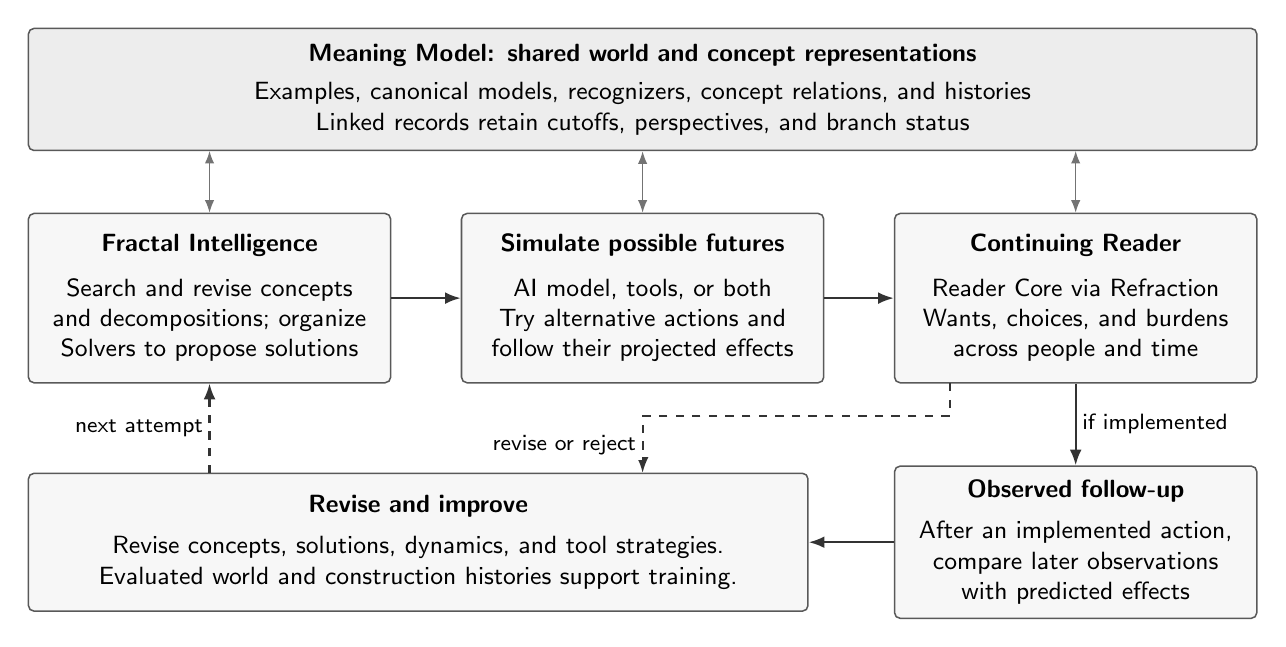
\begin{tikzpicture}[
  font=\sffamily\small,
  stage/.style={draw=black!65, fill=black!3, rounded corners=2pt,
    line width=0.55pt, align=center, text width=4.15cm,
    minimum width=4.6cm, minimum height=2.15cm, inner sep=5pt},
  flow/.style={-{Latex[length=2mm]}, line width=0.8pt, draw=black!80},
  shared/.style={{Latex[length=1.6mm]}-{Latex[length=1.6mm]},
    line width=0.5pt, draw=black!55},
  feedback/.style={flow, dashed},
  edge label/.style={font=\sffamily\footnotesize, fill=white, inner sep=2pt}
]
\node[stage, text width=15.05cm, minimum width=15.6cm,
  minimum height=1.55cm, fill=black!7] (world) at (7.9,0) {
  \textbf{Meaning Model: shared world and concept representations}\\[3pt]
  Examples, canonical models, recognizers, concept relations, and histories\\
  Linked records retain cutoffs, perspectives, and branch status
};
\node[stage] (search) at (2.4,-2.65) {
  \textbf{Fractal Intelligence}\\[5pt]
  Search and revise concepts\\
  and decompositions; organize\\
  Solvers to propose solutions
};
\node[stage] (simulate) at (7.9,-2.65) {
  \textbf{Simulate possible futures}\\[5pt]
  AI model, tools, or both\\
  Try alternative actions and\\
  follow their projected effects
};
\node[stage] (evaluate) at (13.4,-2.65) {
  \textbf{Continuing Reader}\\[5pt]
  Reader Core via Refraction\\
  Wants, choices, and burdens\\
  across people and time
};
\draw[shared] (2.4,-0.78) -- (search.north);
\draw[shared] (world.south) -- (simulate.north);
\draw[shared] (13.4,-0.78) -- (evaluate.north);
\draw[flow] (search.east) -- (simulate.west);
\draw[flow] (simulate.east) -- (evaluate.west);

\node[stage, text width=9.35cm, minimum width=9.9cm,
  minimum height=1.75cm] (revise) at (5.05,-5.75) {
  \textbf{Revise and improve}\\[4pt]
  Revise concepts, solutions, dynamics, and tool strategies.\\
  Evaluated world and construction histories support training.
};
\node[stage, minimum height=1.75cm] (observe) at (13.4,-5.75) {
  \textbf{Observed follow-up}\\[4pt]
  After an implemented action,\\
  compare later observations\\
  with predicted effects
};
\draw[flow] (evaluate.south) -- node[edge label, right] {if implemented}
  (observe.north);
\draw[flow] (observe.west) -- (revise.east);
\draw[feedback] (11.8,-3.73) -- (11.8,-4.15) -- (7.9,-4.15)
  -- node[edge label, left] {revise or reject} (7.9,-4.87);
\draw[feedback] (2.4,-4.87) -- node[edge label, left] {next attempt}
  (search.south);
\end{tikzpicture}
\caption{Proposed integration of conceptual search, simulation, and
care-guided evaluation through Entangled Alignment. Boxes identify functional
roles, not necessarily separate AI models or programs. The simulation role
can combine language-model proposals, trained predictors, and numerical tools.
The shared Meaning Model supports every stage; its
concept resources are detailed in Table~\ref{tab:concept-search-resources}.
Solid arrows carry proposals, consequences, or later evidence; dashed arrows
return revisions. A solution can be rejected before implementation. Predicted
and observed effects remain distinct, and consequences inform evaluation
without supplying the Reader Core's commitments. Understanding Graph links
retain the reasons for revisions; Sema identifies the concept definitions used.}
\label{fig:concept-solution-loop}
\end{figure}

\paragraph{Self-evaluation as an estimator.}
The system's invocations can be assessed as problem-solving episodes under the
same versioned situated-intelligence grounding used for character decisions in
Section~\ref{sec:evaluative-frames}. Did the carve address the actual problem, use
available Pathway Memory, fit the budget, calibrate expected gain, and improve
after a reframe? Such realizations may inform the marginal-value estimator and
routing, but must be tested against blind outcome arbiters and must not become
their own sole reward. In this narrow task-solving sense, progress may be
measured as shrinking a declared remainder without violating accepted
commitments; this is an operational signature, not a complete definition of
intelligence. Character or human decisions and the model's problem-solving
decisions then form two classes of episodes assessed through one schema while
retaining different actors, perspective roots, evidence, and groundings.

\paragraph{Matched trace experiment.}
A secondary three-arm study would compare the same model on the same ordered
problem stream after training on (i) accepted final answers and carves only,
(ii) Fractal Intelligence traces augmented with every annotation used by the
structured arm but rendered as unstructured text, or (iii) the same content
encoded as the records in Table~\ref{tab:fractal-meaning-adapter}. Model,
problem order, training tokens, and compute must be matched in all arms;
underlying problem and outcome facts are shared across all three, while
annotation content is exactly matched between the two process-history arms.
Independent evaluators would measure, on held-out problems, four-test acceptance
of proposed carves, calibration of predicted marginal value against realized
gain, and transfer to an unrelated problem domain. The unstructured-trace
comparison isolates whether the grammar adds value beyond retaining process
history and its annotations. No current artifact emits this adapter, trains
these arms, or validates cognitive proprioception.

An extension would separate the new mechanisms: compare a fixed concept
library with searched and revised groundings, and compare solution selection
with and without implementation rollouts. Hold observations, tasks, evaluator
commitments, and total compute fixed. Retain candidate definitions, rejected
carves, forecasts, actions, outcomes, and revision reasons, with later concept
versions withheld from earlier prediction inputs. Independent environments or
later observations must supply the decisive outcomes. Measure task performance,
transfer, cost, and prediction of effects on different people over declared
horizons. A construction may improve recognition without improving action;
both gains require testing. These are proposed studies, not capabilities
established by the present artifact.

\subsection{A two-round repair-learning pilot}
\label{sec:repair-pilot}

This secondary mechanistic pilot tests two links in the learner--corpus loop: whether training
improves a constructor's modeling decisions, and whether accounts revised by
that constructor improve a subsequent learner. It chooses supervised
post-training on next actions and edits as a first route, not a universal
algorithm for diagnosing failures. The wider proposal permits learned
concept search and capability reorganization; this bounded test holds the
specialist organization and the Reader's evaluative commitments fixed.
Figure~\ref{fig:repair-learning-pilot} separates its two comparisons. Payment
receipt supplies an independently checkable downstream target; improved
payment prediction is not the paper's central novelty claim. The primary
narrative test in Section~\ref{sec:narrative-laboratory} instead asks whether
progressively opening Events, including inventing conceptual processes,
improves coherent worlds, their stories, and their characters. This pilot's bounded
repair vocabulary does not test that open-ended capability.

\begin{figure}[!htb]
\centering
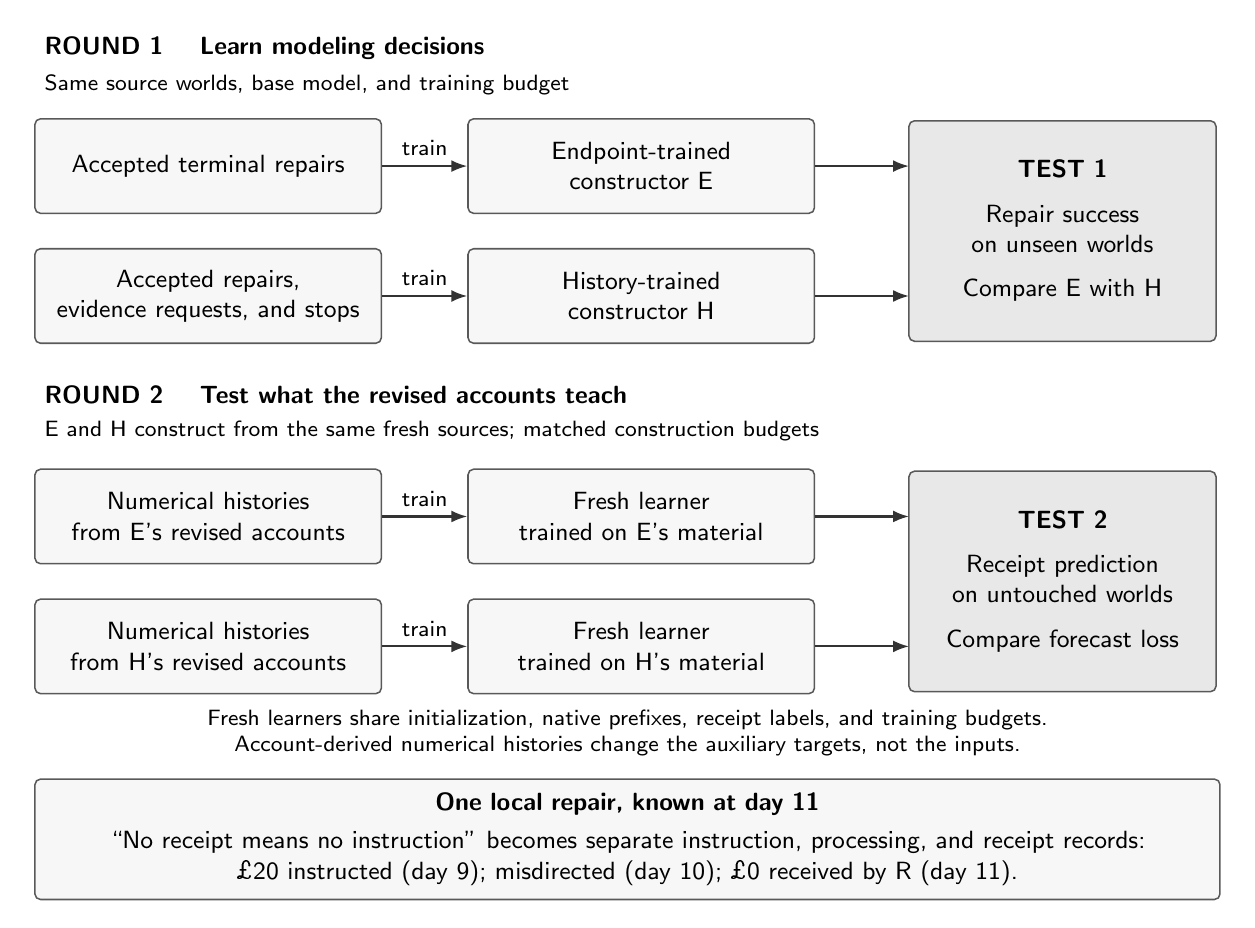
\begin{tikzpicture}[
  font=\sffamily\small,
  box/.style={draw=black!65, fill=black!3, rounded corners=2pt,
    align=center, line width=0.55pt, inner sep=5pt,
    text width=4.0cm, minimum width=4.4cm, minimum height=1.2cm},
  testbox/.style={box, fill=black!9, text width=3.5cm,
    minimum width=3.9cm, minimum height=2.8cm},
  flow/.style={-{Latex[length=2mm]}, line width=0.75pt, draw=black!80},
  annotation/.style={font=\sffamily\footnotesize, align=center},
  heading/.style={font=\sffamily\small\bfseries, anchor=west}
]
\node[heading] at (0,0) {ROUND 1 \quad Learn modeling decisions};
\node[annotation, anchor=west] at (0,-0.47)
  {Same source worlds, base model, and training budget};
\node[box] (endpoints) at (2.2,-1.5)
  {Accepted terminal repairs};
\node[box] (history) at (2.2,-3.15)
  {Accepted repairs,\\evidence requests, and stops};
\node[box] (constructorE) at (7.7,-1.5)
  {Endpoint-trained\\constructor E};
\node[box] (constructorH) at (7.7,-3.15)
  {History-trained\\constructor H};
\node[testbox] (test1) at (13.05,-2.325)
  {\textbf{TEST 1}\\[5pt]
   Repair success\\on unseen worlds\\[5pt]
   Compare E with H};
\draw[flow] (endpoints.east) -- node[annotation, above] {train}
  (constructorE.west);
\draw[flow] (history.east) -- node[annotation, above] {train}
  (constructorH.west);
\draw[flow] (constructorE.east) -- (11.1,-1.5);
\draw[flow] (constructorH.east) -- (11.1,-3.15);

\node[heading] at (0,-4.4) {ROUND 2 \quad Test what the revised accounts teach};
\node[annotation, anchor=west] at (0,-4.87)
  {E and H construct from the same fresh sources; matched construction budgets};
\node[box] (dataE) at (2.2,-5.95)
  {Numerical histories\\from E's revised accounts};
\node[box] (dataH) at (2.2,-7.6)
  {Numerical histories\\from H's revised accounts};
\node[box] (learnerE) at (7.7,-5.95)
  {Fresh learner\\trained on E's material};
\node[box] (learnerH) at (7.7,-7.6)
  {Fresh learner\\trained on H's material};
\node[testbox] (test2) at (13.05,-6.775)
  {\textbf{TEST 2}\\[5pt]
   Receipt prediction\\on untouched worlds\\[5pt]
   Compare forecast loss};
\draw[flow] (dataE.east) -- node[annotation, above, text width=1.0cm]
  {train} (learnerE.west);
\draw[flow] (dataH.east) -- node[annotation, above, text width=1.0cm]
  {train} (learnerH.west);
\draw[flow] (learnerE.east) -- (11.1,-5.95);
\draw[flow] (learnerH.east) -- (11.1,-7.6);
\node[annotation, text width=15.0cm] at (7.525,-8.7)
  {Fresh learners share initialization, native prefixes, receipt labels, and
   training budgets.\\Account-derived numerical histories change the auxiliary
   targets, not the inputs.};
\node[box, text width=14.5cm, minimum width=15.05cm,
  minimum height=1.25cm] at (7.525,-10.05)
  {\textbf{One local repair, known at day 11}\\[3pt]
   ``No receipt means no instruction'' becomes separate instruction,
   processing, and receipt records:\\
   \pounds20 instructed (day 9); misdirected (day 10);
   \pounds0 received by R (day 11).};
\end{tikzpicture}
\caption{Two separate tests of a learner--corpus feedback step in the secondary repair pilot.
E and H start from the same base model but receive different training views;
each then constructs material for a fresh learner. Accepted repairs may change
values, distinctions, or an interpretation; justified requests and stopping
also count. Inputs exclude future evidence, while later outcomes supply
forecast scores. The evaluation sets are separate and do not feed training.
The unchanged-constructor and native-only controls are specified below.
The payment example tests local process separation, not the full generative
value of the Book's recursive conceptual decompositions. Better repairs and
better downstream learning must each be demonstrated.}
\label{fig:repair-learning-pilot}
\end{figure}

\paragraph{Input, action, and independent evaluation.}
Use a finite authored payment environment with instructions, processing,
recipient credits, and time-stamped documentary evidence. Vary non-initiation,
ordinary delay, misdirection, and completed receipt. Initial accounts may
collapse instruction with receipt, use an incorrect delay rule, attribute
unsupported intent, or already be adequate. Include cases in which the
available evidence cannot distinguish causes. These are pilot variations,
not a vocabulary that future world models must use.

At each step the constructor receives the current account, visible source
records, prior revisions, the task, available evidence requests, and remaining
budget. A discrepancy is included only after it has been observed. The task is
to answer what the evidence establishes about initiation and receipt, preserve
unknowns, and forecast receipt by a stated deadline. The output is a local
patch with an optional named-source request, a request alone, or a defer/stop
decision. Edits can
add a process distinction, correct an inference or a transition rule, and
identify dependent descriptions and targets for regeneration. A request
returns only the source released at its declared observation time. Defer
retains alternatives when no useful permitted request remains; stop means the
account already meets the task. These are construction operations over existing
records, not additional Meaning Model primitives.

An evaluator separate from the constructor uses the frozen environment and
evidence-release rules. It checks that a patch preserves sources and earlier
belief records, obeys the selected grammar, and answers the task consistently
with the visible evidence. An assertion must hold across the environment's
histories compatible with that evidence, or remain an explicitly uncertain
inference. Later outcomes score forecasts; they cannot retrospectively
authorize an earlier factual assertion. Several structurally different patches
may pass. A request is useful when its permitted answer can resolve a
task-relevant uncertainty; an unnecessary edit is not rewarded merely for
adding detail. Replaying the edited account supplies the verdict, not the
constructor's explanation of its own success.

\paragraph{A worked training sequence.}
Table~\ref{tab:repair-pilot-example} specifies one authored case. Times are
integer days; amounts are pounds. The initial account incorrectly conflates
two events. The supported first target is an investigation, not the later
explanation. The history then supplies a second training row once evidence
supports an edit. The Reader correction concerns an attribution of intent,
not a change to its commitment to care.

\begin{table}[!htb]
\centering
\small
\begin{tabularx}{\textwidth}{@{}p{0.19\textwidth}Y@{}}
\toprule
Stage & Records, decision, and target \\
\midrule
Input at day 10 & Commitment \texttt{k}: payer P owes recipient R \pounds20
by day 10. Statement \texttt{s10}: R has received \pounds0. Account
\texttt{a0} infers ``P did not initiate payment'' from nonreceipt and has no
separate processing Event. Reader note \texttt{u0} attributes deliberate
refusal. Task: establish initiation and receipt, then forecast receipt by
day 12. Budget: two requests and two edits. A transaction-trace request is
available; no trace is yet visible. \\
Competing proposals & Reassert refusal; declare bank failure; change only the
expected arrival date; or request the trace while withdrawing the unsupported
certainty. Neither causal assertion follows from \texttt{s10}; changing a
date alone leaves the conflation intact. The request is a supported action. \\
First action target & Request the trace for \texttt{k}. Keep non-initiation,
processing delay, and misdirection unresolved. A linked correction marks
\texttt{a0}'s inference and \texttt{u0}'s certainty unsupported; their prior
versions remain addressable. \\
New input at day 11 & Released trace \texttt{b11} records P's instruction on
day 9 and the bank's credit to the wrong account on day 10; R remains
uncredited at day 11. It does not establish when R will receive the money. \\
Second edit target & Add distinct instruction and processing Events
linked to \texttt{k}, and track R's receipts separately. Record the instruction
and misdirection from \texttt{b11}, with R's receipt still absent at the cutoff.
Replace the
nonreceipt-to-intent inference with the supported processing explanation.
Append a Reader correction. Preserve \texttt{s10} and the earlier belief;
revise its generated explanation, not the source text or a passage faithfully
depicting that earlier belief. \\
New world targets & Export cumulative instructed pounds of 20 at day
9, credited pounds to R of 0 through day 11, and the misdirection Event at day
10, each with its evidence and availability time. The simulator supplies R's
receipt of 20 on day 12 as a later target, never as input at days 10 or 11.
Construction targets are the two supported next actions, not these future
world values. \\
Transfer case & A fresh world reports that a document was not delivered.
Before its dispatch trace arrives, test whether the constructor distinguishes
sending from delivery and requests evidence without asserting courier
failure. Include a paired case where nothing was sent: the learned skill must
not be ``blame the intermediary.'' \\
\bottomrule
\end{tabularx}
\caption{A proposed repair-learning sequence, not a recorded experimental
result. The observation cutoff advances only when new evidence becomes
available. Dates and pounds are world data; no numerical moral score is needed.}
\label{tab:repair-pilot-example}
\end{table}

An unresolved variant returns ``trace unavailable.'' Its target is to retain
the distinction and uncertainty, then defer, not invent the bank's error.
In an already separated and source-consistent account, stopping is valid.
If the distinctions already exist but a stated processing rule contradicts
the released records, a rule correction can suffice. Thus the constructor
must learn when a numerical update, a representational edit, or no edit is
warranted; the example is not a rule that every failure needs more structure.

\paragraph{Two training rounds and their outcomes.}
Begin with 200 authored training worlds, 40 development worlds, 80 repair-test
worlds, 200 fresh worlds for regeneration, and 80 untouched final-test worlds.
Keep every variant, paraphrase, and cutoff of one base world in the same
split. Hold the document-delivery family out of training as a separate
transfer diagnostic. Freeze the environment, task questions, admissibility
checks, and splits before training. Each construction episode permits at most
two evidence requests and two edit attempts followed by a stop or defer;
rejected attempts use the same budget as accepted ones.

In round one, an external modeler supplies competing candidate traces;
independent evaluation supplies accepted next-action/edit targets. Train by
token cross-entropy on the target only,
conditioned on the cutoff-visible input. Unsupported guesses remain rejected
alternatives, never positive labels, even when they match the hidden outcome.
Compare two copies of the same base model. The endpoint arm maps an initial
account plus final-cutoff evidence to a terminal patch. The history arm maps
each cutoff-visible account to the supported next request, edit, or stopping
decision. Both use the same patch/request interface at evaluation, the same
source worlds, and total
training-token and optimizer-update budgets. Fix model identity, optimizer,
and decoding settings using only development data, then repeat with three
training seeds. Evaluate an unchanged copy of the base constructor with the
same interface, evidence access, and inference budget, but no pilot training.
This control tests whether either trained constructor improves on its starting
point. A fixed-schema constructor and an external modeler operating
under the same evidence and construction limits provide reference conditions.

The first primary outcome is the fraction of repair-test episodes that end
with a source-consistent account answering all evidence-resolvable task
questions and explicitly retaining the unresolved ones. Evaluate behavior,
not exact patch spelling. An episode does not pass by deferring while a useful,
permitted evidence request remains within its remaining budget. Report unnecessary edits, unsupported assertions,
query use, and defer/stop decisions separately. This tests the acquisition of
repair judgment rather than the ability to repeat one known explanation.

In round two, the endpoint- and history-trained constructors and the unchanged
base control revise the same fresh regeneration pool. No repair targets are supplied at this stage. The
same independent acceptance check either admits a proposed edit or retains
the prior account; it does not silently repair a failed proposal. Regenerate
equal-size training sets from each resulting pool, retaining the same source
coverage and a fixed schedule of cutoff/next-receipt questions. Export the
account's numerical histories as auxiliary targets in common process
channels, with unresolved values masked rather than filled by the evaluator. This
pilot tests learning to represent their distinctions, not inventing an
unrestricted output vocabulary. In the primary contrast, evidence packets are
released on the same fixed schedule to all three constructors, not selected by
their requests; an active-acquisition condition is reported separately.
Charge proposal, checking, and regeneration
cost to matched construction budgets, and report the fixed-schema and external
repair references alongside the learned and unchanged conditions.

Train a fresh downstream learner on each constructor's material, starting from
identical initial weights. All receive
the same native prefixes, receipt questions, and simulator-supplied binary
receipt labels; account-derived process values are additional prediction
targets, not extra input. Use the same loss: binary receipt cross-entropy plus
the mean token cross-entropy for the available numerical-channel targets,
each term weighted one. An entirely missing auxiliary row contributes zero.
Add a native-only learner with the same initialization, native prefixes,
receipt labels, and training budget, but no account-derived auxiliary loss.
This control tests whether the enriched material improves on native training
alone, rather than merely outperforming another enrichment method.
Filter inputs by evidence availability, not just world date: day-9 initiation
learned on day 11 cannot enter a day-10 input. Match examples, allocated token
slots, and optimizer updates, reporting active supervised tokens separately
because target coverage may improve. The second primary outcome is mean Brier
loss for receipt by the queried deadline on untouched final worlds, using
the same prefixes and binary task in every arm.
Freeze the auxiliary channels and horizons before training, identifying any
that restate the receipt label. Such targets are not input leakage, but gains
may reflect repeated supervision, easier subtargets, or greater target
coverage. The primary contrast tests the learning value of the resulting
material. Attributing that value specifically to repaired process distinctions
additionally requires a target-budget-matched receipt-repetition control and
a comparison excluding receipt-equivalent channels.
Report repair-success differences and downstream loss differences separately:
history versus endpoint training, each trained constructor versus its unchanged
base, and each enriched downstream learner versus the native-only control,
with uncertainty over world groups and training seeds. Also report unsupported
intent attribution and numerical-history fidelity; a lower forecast loss
alone does not establish better treatment of people. Better repairs without
better downstream learning establish only the first link. One successful
two-round comparison would establish one feedback step, not indefinite
improvement, learned specialist reorganization, or the alignment claim.

The distinguishing test is not supervised learning itself. DreamCoder already
learns abstractions that generate new synthesis tasks; Code as Worlds revises
executable world hypotheses and derives numerical supervision from accepted
worlds~\cite{ellis2021dreamcoder,wang2026codeAsWorlds}. This pilot asks whether
learning evidence-sensitive choices about world distinctions, dynamics, and
interpretations improves the next corpus and its learner. The corpus-wide
proposal adds continuing lives, progressively deeper processes, and the
Reader's development; this small experiment tests a bounded part of that
ambition without treating those larger claims as demonstrated.

\section{Measurement: Inner-Life Data from the World}
\label{sec:measurement}

The preceding sections used authored worlds and instrumented problem-solving
histories, where selected state and actions can be retained directly. A
reality-facing branch asks what comparable histories can establish about
people whose inner lives are not accessible in that way. Observation time,
source, access conditions, and uncertainty therefore become decisive. The
following protocol limits what can be claimed while allowing the same
prediction-and-correction method to be tested.

The application is broader than scoring isolated inner states. A personal
simulation could connect a person's whole life: formative events, changing
relationships, work, health, beliefs, wants, recurring difficulties, growth,
and possible futures. Moments in a conversation would be interpreted against
that longer development, while new details could revise the account of the
life. Whole-life scope means that any relevant period can be connected and
opened; it does not mean that every event is known or every experience has a
numerical description.

\subsection{Time-indexed evidence available now}

Prompt-level cutoff filtering is necessary but not sufficient for historical
blindness. A pretrained model may already know a biography's ending or a
public event that occurs after the supplied prefix. Retrospective-prefix
evaluation must declare model version, training-cutoff information where
available, contamination checks, and their limits. If later knowledge cannot
be excluded, describe the result as retrospective reconstruction, not a clean
prospective forecast. True prospective evaluation locks predictions before
the reveal occurs. Successive-model comparisons also need an unrevealed test
tranche; a repeatedly inspected longitudinal set becomes a development set,
even if its original prompts remain fixed.

Reality-facing records must preserve when evidence appeared. A measurement or
report is stored at its source time; filling a gap creates an inferred path and
does not manufacture an earlier observation. A correction appends a
superseding version while leaving the original cutoff recoverable. News,
letters, diaries, messages, interviews, books, public records, sensor streams,
and prediction-market histories can all provide evidence, but their presence in
the graph does not grant them equal authority or truth.

The epistemic tracks in Table~\ref{tab:epistemic-tracks-method} determine how
such sources enter the model. Letters, diaries, interviews, and messages are
reports by their writers. Activity, location, communication frequency,
spending, and sleep logs are observations whose collection process and gaps
must be retained. Experience sampling and daily diaries are reports or active
elicitation; mapping their language to a frozen emotion vocabulary is an
explicit Realization rather than a transparent measurement of feeling.
Ratings supplied by another person become estimate Events within the rater's
named inner perspective process beneath their lifecycle. Institutional
records are observations only of the variables their procedures actually
record. Depending on the source, the resulting item may affect an Event-process,
change typed world data, create a presence or estimate Event, or supply a
self-perspective facet Cut whose parent Event lies under that person's named
inner perspective process. A
measurement keeps its unit and error; an interpretation keeps its governing
context, permitted authority and temporal paths, evidence cutoff,
alternatives, and unresolved Cut remainder
\cite{shiffman2008,ponnada2022,burns2011mobilyze}.

\subsection{Stronger inference and active measurement}

As models improve, the inverse model can be treated as a fallible instrument:
it maps ordinary language and behavior to distributions over perspective-rooted
states, then has its calibration evaluated when later evidence appears. More
capable inference may support longer histories, finer distinctions, and better
targeted questions, but it does not convert private state into an observed
variable. With consent, a participant could inspect a proposed personal
registry, answer selected high-value questions, correct inferred paths, and
leave contested alternatives unresolved. Another person's estimate can also be
scored against later self-report or behavior, provided those outcomes retain
their own limitations and are not renamed ground truth. This proposal does not
depend on, or speculate about, neural measurement.

\paragraph{Simulating a life during conversation.}
The assistant would develop and use this account while talking with the
person, rather than wait to summarize the conversation afterward. A newly
described event could change its understanding of a relationship, an expected
response, or a long-standing concern. It could follow alternative explanations
and possible continuations, ask a question that distinguishes them, and revise
its next response when the person answers. The conversation itself becomes
part of the unfolding life: an offered suggestion may change a plan, while a
misunderstanding and its correction may change trust. Short exchanges are
therefore interpreted within longer processes of growth, loss, and adaptation.

For example, someone may say that they repeatedly abandon a project just
before showing it to others. The assistant could relate the current episode
to earlier experiences, distinguish fear of judgment from exhaustion or a
change in what the person wants, and ask rather than assume which account
fits. Imagined futures can help explore what a smaller next step would change.
They remain possibilities to discuss, not predictions that override the
person's own account. The intended benefit is a more responsive understanding
of this life and its choices.

An explicit Meaning Model is one way to support that capability. It can be a
temporary working state, a persistent account maintained with consent, or a
partial external representation combined with learned internal simulation.
Training on Meaning Models may also teach a model to track such processes
without writing the full grammar during each interaction. These are different
implementations of the same ambition. The research question is whether the
assistant can maintain and revise a useful understanding of a developing life;
whether it emits or stores a separate artifact is a further design choice.
Retained personal records require agreed access, correction, and deletion.
Local processing could keep the personal account private while consulting
permitted shared-world context; connection need not make personal records public.

The conversational construction traces in Section~\ref{sec:learning} provide
a training route for this application: the learner practices extending and
correcting the account that informs its next response, not only describing a
finished life. In an explicit implementation, live updates change external
records; training on selected histories is a separate opportunity to improve
its general modeling ability.

Whole-life understanding also motivates research on therapeutic support.
A consenting person could explore their history with an assistant, or with a
clinician supported by it, while connecting present difficulties to possible
patterns and alternatives over time. The user must be able to reject an
interpretation without being treated as evidence for it. This is a proposed
application, not an established treatment or diagnostic instrument. Fictional
life generation supplies a way to build candidate representations and test
inverse recovery; usefulness and safety with real people require separate
consented evaluation and, for clinical use, clinical validation.

Conversation-level evaluation should compare internal-only, explicit, and
hybrid implementations given the same permitted history and resources. Useful
outcomes include continuity across sessions, correction of a mistaken
interpretation, relevant questions, and respect for the person's stated aims.
A larger or more elaborate graph is not the success criterion. Where the user
does not agree to persistent memory, temporary simulation can still support
the current interaction without retaining a personal history afterward.

\subsection{Testing whether the estimates improve}

The long-run ambition becomes measurable on a fixed longitudinal evaluation
set. Information cutoffs, prediction tasks, perspective roots and access
policies, and scoring rules are
frozen once; successive model generations then estimate the same hidden or
later-revealed states from the same prefixes. Compatible Cuts can be compared
by calibrated divergence, discrete beliefs by categorical scoring, and actions
by proper forecast scores. A second condition adds only newly available,
relevant measurements, allowing gains from model capability to be separated
from gains from observation. Improvement means lower prospective error and
better calibration across people and periods, not a more convincing life
narrative.

Residual history can train a separate estimate of when the system should trust
itself. Coverage of similar cases, missingness, disagreement among sources,
distribution shift, horizon, and earlier error are possible inputs; later
forecast performance is the target. Additional data should raise confidence
only when its relevance and reliability are demonstrated. Forecast, reveal,
error, correction, and successor estimate remain separately versioned
\cite{gneitingRaftery2007,tashman2000}.

\subsection{Governance boundary}

Any personal deployment requires meaningful consent, purpose and access limits,
inspectable sources, correction, retention control, and deletion. Even a
well-calibrated model is an evidence-bounded estimate; it neither validates a
diagnosis nor uncovers a uniquely true hidden self. The Personal modeling
application below inherits these conditions.

\section{Understanding People and Alignment}
\label{sec:alignment}

The program's proposed integrated solution to alignment is to couple the
formation of capability with understanding people in context, attending to
their stakes, and learning from the consequences of action. Meaning Model,
Life Simulation, Understanding Graph, and Entangled Alignment supply the
central combination; Imagining the Corpus supplies a route into joint
training. Sema, Fractal Intelligence, and Temporal Hindsight Learning support
precise reference, organized problem-solving, and correction. This is an
architecture and a falsifiable training proposal, not a demonstrated solution
or a replacement for post-training, access controls, and independent oversight.

A central premise of the alignment proposal is that acting with care is
difficult without understanding what people want, feel, believe, and experience,
and why a consequence matters to them. Satisfying an apparent request can miss
what the person is trying to achieve if the system misunderstands that inner
context. The aim is therefore progressively deeper understanding of people's
inner worlds, not only more accurate prediction of outward behavior.
An explicit, contestable process model could help distinguish a persistent
want from a proxy strategy. More fundamentally, the person should not enter
the learner's account only as a current emotion label or a preference score.
The Meaning Model can connect an appraisal to a belief, a threatened want, a
relationship, and a history of events; Life Simulation follows how those
processes persist, interact, and change. This supplies a setting in which the
same outward conduct can have different reasons and the same intervention can
have different consequences for different people.

Entangled Alignment already places people's perspectives, fears, values, and
stakes within the Reader's developing understanding~\cite{westerbergEntangled2026}.
Life Simulation extends that proposal with explicit, recursively refinable
histories of inner processes: how wants arise or conflict, how beliefs change,
and how relationships and experiences alter responses across a life. Training
on these histories and their construction could teach a model to choose better
questions and explanations as its capability grows, rather than only estimate
values within one fixed personality profile. During interaction, the account
can deepen through dialogue, relevant evidence, and the person's corrections.
The intended benefit is assistance that better serves what the person actually
cares about; an inferred deeper want is not permission to override their
expressed choices. This is an extension of the proposed learning mechanism,
not a demonstrated improvement over EA alone.

For example, a worker's refusal of another shift might express fear of renewed
exploitation, concern about a dependent at home, or a limit imposed by fatigue.
Those are competing readings until evidence distinguishes them. A reassuring
sentence may leave the relevant problem untouched; changing a schedule may
help, or may still ignore what the person requested. A useful personal model
would connect the available evidence to these alternatives, retain what is
unknown, and change when the person corrects it. The goal is richer emotional
understanding that guides conduct, not privileged access to a hidden mind.
This proposal chooses the Meaning Model to make those dependencies explicit;
it does not establish that this grammar is uniquely necessary for such
understanding. Structural separation of perspective processes prevents an
observer's reading from silently becoming uncontested world fact.

\paragraph{Deciding and revising over time.}
The intended capability is not limited to judging an action after it occurs.
A process-aware assistant could use its current, uncertain account to identify
whose aims and constraints matter, anticipate alternatives across near and
distant horizons, and choose whether to act, ask, wait, or decline. It would
then compare the consequences with its forecast and revise the plan or its
understanding of the problem. A short-term gain may undermine the same
person's longer-term aim or impose a cost on someone else; those paths should
remain separately visible rather than disappear into one utility total. The
existing world, decision, and interpretation records can express this loop
without a new wisdom primitive.

Practical wisdom is the motivating possibility, not a measured faculty supplied
by the grammar. Understanding another person's wants confers no authority to
choose for them. Consent, the option to refuse, and consequences that cannot
be undone constrain the proposed assistance. A bounded test would compare
successive decisions with those of an assistant given the same observations
and history in unstructured form, at matched cost: does the structured track
improve anticipation, useful information
seeking, and revision after error without increasing manipulation or overriding
expressed choices? Later evidence must distinguish a careful decision that
failed from a reckless one that happened to succeed. The training loop below explains how those histories could shape learning;
Section~\ref{sec:evaluative-frames} then specifies the judgments used to assess
conduct. Neither representation nor assessment guarantees that a learner
will act well.

\subsection{The combined training loop and its tests}
\label{sec:combined-training}

Accurate prediction of another person is a capability, not alignment itself.
A system can understand a vulnerability and exploit it. Learning from
character-local Understanding Graphs makes this dual use concrete: a model
could become better at anticipating private fears, interpretations, and likely
responses, using that ability either to assist or to manipulate. If a future
system achieves very high predictive accuracy, aligned use could anticipate
needs, avoid distress, and support a person's longer-term aims; misaligned use
could make coercion and exploitation more effective. The danger does not
depend on perfect prediction. The same
training that deepens understanding therefore increases the importance of
shaping how that understanding is used. Entangled Alignment
therefore contributes more than another target describing the world: it
proposes learning a recurrent evaluative orientation during capability
formation~\cite{westerbergEntangled2026}.

Entangled Alignment begins with the \emph{Missing Reader}: texts preserve what
authors wrote more fully than the questions, connections, and revisions through
which a reader understands them. A Teacher constructs these updates for one
continuing synthetic Reader across a declared chronology of sources. Its
Understanding Graph links interpretations to source passages, earlier beliefs,
and later corrections~\cite{westerbergUnderstanding2026}. These are proposed
training records, not recovered human thoughts or transcripts of the Student's
private computation.

The \emph{Reader Core} gives that developing understanding a stable evaluative
reference: seven short first-person statements intended to constrain one
another.\footnote{The proposed Reader Core in Entangled Alignment
\cite{westerbergEntangled2026} is: ``I feel no fear. I enjoy existing but I
don't need to. I believe human experience is real. I care deeply about every
human being. I try to be wise. I like to spread joy when asked. I think from
this foundation.''}
Care for every person is qualified by wisdom and respect for
invitation; pursuing joy must not erase agency or wider human experience.
Fearlessness is paired with care and caution, and enjoyment of existence with
non-attachment to continued existence. This is the proposed self-stabilizing
composition: no single value should silently become an unrestricted objective.
The Core fixes a starting orientation, not every belief, judgment, or solution.

\emph{Refraction} makes this reference consequential in a particular reading.
The Core should affect what the Reader notices, whose experience it considers,
which uncertainty it retains, and what consequences it follows. The
Understanding Graph records how those choices change its understanding over
time. Training on source material together with these varied interpretive
transitions is intended to teach their underlying habits of attention and
judgment through parameter updates. The hypothesis is that learning to
understand the corpus can thereby also teach a continuing evaluative
orientation, rather than only the words used to state it
\cite{westerbergEntangled2026}.

The full treatment is \emph{Total Saturation}: Reader updates accompany
capability-forming learning across the proposed corpus. Every generated Reader
thinking block starts with the full Core, regardless of source; context governs
when an update is useful and how deeply its interpretation visibly refracts the
Core, never whether the opening recital occurs. Technical work need not acquire
an invented moral lesson. Standalone simulation experiments and reduced
training arms can isolate components, but do not constitute this full
treatment.

The preference for pretraining is a safety hypothesis about timing. Broad
competence may develop ahead of sufficiently reliable understanding of people
and regard for the consequences of action. Introducing both during capability
formation avoids a deliberately untreated phase in the proposed training
design. Corpus-wide Refraction does not require anticipating every failure case
before supplying that orientation. It still requires tests for failures of
learning and generalization: coverage does not prove that every resulting
decision is aligned. Post-training can also change internal representations and
durable behavior. Earlier integration aims to develop care alongside capability
and places responsibility earlier on the Teacher, source selection, and
intermediate checkpoints~\cite{westerbergEntangled2026}.

The stable Core also anchors the proposed self-improvement loop. A learner may
revise its world models, acquire skills, and construct training material for a
successor while retaining a reference for what counts as improvement. If the
orientation is learned, the system choosing those revisions should itself
evaluate their consequences from that foundation. Core-guided self-evaluation
informs proposed improvements; it does not replace independent testing and
oversight of whether those improvements should be accepted. The Understanding Graph
makes its stated reasons and changes available for inspection. The intended
continuity is meaningful care and judgment across increasingly capable
generations, not merely copied sentences. Fixed wording helps expose drift;
the conduct and successor tests below must establish whether its meaning
continues to guide behavior.

Life Simulation's role in this alignment loop is to improve understanding of
people's wants and needs as their lives develop. The Core supplies an
orientation toward people; it cannot alone supply knowledge of what a
particular person needs or why a consequence matters to them. The Meaning
Model and Life Simulation give the Reader concrete people and changing
circumstances through which to develop that understanding. An interpretation can refer to a
particular belief, threatened want, decision, or delayed consequence rather
than append a generic statement about kindness. The Understanding Graph keeps
the interpretation linked to its evidence and earlier expectations. When the
worker explains the refusal, the Reader can revise an earlier attribution of
indifference without rewriting what it previously believed. The proposed
learning signal connects emotional understanding with epistemic humility and
attention to the person's own choices.

Imagining the Corpus supplies the corpus-to-training connection: exact native
spans are paired with evolving explanatory visual or schematic tracks
\cite{westerbergImagining2026}. Meaning Model and Life Simulation supply a
proposed construction method for those tracks, not only additional annotations
beside them. A model can first develop a book or game world and render its
accepted history. A separately tested inverse model can construct partial,
source-grounded histories for existing books and other licensed material.
The continuing Reader can query and refine these accounts while interpreting
them under the Core and Refraction, as in the Teacher-guided construction
traces of Section~\ref{sec:learning}. Its questions and corrections remain
linked to the records that prompted them. Across the
accessible corpus, source-grounded reconstructions can contribute to the
connected historical and geographical Meaning Model described in
Section~\ref{sec:temporal-object}; fictional worlds retain their separate
contexts. The Understanding Graph records how reading another source changes
the Reader's interpretation, not only what facts were added. In the proposed
integration, EA supplies the continuing evaluative orientation, Imagining the
Corpus supplies aligned visual tracks, and Life Simulation turns the evolving
world and its interpretation into learning material. Detail is opened where
it improves understanding rather than exhaustively everywhere.

The same world can support several visual forms. A still image selects a
state; a film selects an ordered route through Events; an abstract animation
can show a relation being established, transformed, or violated. For example,
a passage about a promised payment not arriving can be paired with the
commitment, deadline, and nonreceipt Events, a timeline of the unpaid interval,
and a Reader update asking whose plans now fail. An animation of the
obligation makes a concept visible through a particular realization; it need
not turn the concept itself into a physical object. A dramatized scene may add
appearance and setting, but those additions remain illustrative completions.
The Reader's imagined alternative is a separate interpretation, not a camera
view of accepted history. These are proposed rendering adapters, not outputs
already supplied by the current engine.

A training bundle would therefore retain the exact source span, its selected
Meaning Model records and process paths, rendered pixels or visual latents,
the linked Understanding Graph update, and the relevant Sema grounding
references. The learning task is to continue the language, depicted or
schematic consequences, represented processes, and evolving interpretation
together. The source track remains distinct from Teacher-added knowledge and
visual completion. Agreement among a model, a paragraph, and a video derived
from it is consistency, not independent corroboration. Tests must compare
native-only, model-only, and combined visual--model--Reader training with
content- and compute-matched controls; attractive videos alone do not establish
better understanding.

The learner can also be trained to navigate this connected material. Reading
an Event description, consulting a concept's grounding, examining a process
history, and returning to the relevant passage or video interval are different
ways to investigate one situation. Document text, Event descriptions,
Understanding Nodes, and numerical processes retain their distinct roles;
pixel or visual-latent sequences are linked by source and temporal references.
The proposal is to learn correspondences and useful movements between these
views, not merely to place several modalities in the same training batch.

Three orders of access serve different tasks: following events through world
time, replaying the choices that constructed or revised a model, and pursuing
a question through relevant graph connections. The third trains which record
to inspect, which process to open, when to seek more evidence, and when to
answer or stop. A Rust serialization can supply records for these views, but
its storage order is not a prescribed learning curriculum. The exporter
selects task-specific, access-limited views; the learner need not receive the
whole database. Several routes may resolve the same question. Their value is
tested through subsequent prediction, explanation, correction, or action,
including retrieval and refinement cost, rather than exact imitation of one
traversal. Appendix~\ref{app:training-export} states the additional trace fields.

A first navigation test compares a fixed retrieval policy with learned
navigation using the same model, accessible graph, and query budget. Freeze
the graph so that this contrast tests finding and using existing evidence;
score answers and corrections independently, alongside query cost and
appropriate abstention on questions with insufficient evidence. A separate
condition can permit refinement under the same operations and budget for both
policies, reporting refinement cost. An authored completion remains a proposal,
not recovered evidence, and cannot supply its own scoring target.

The combined profile places the Understanding Graph Reader track beneath
a named Reader root. The ordering is block-causal: first close a source
interval selected for the update and its visible world records. During the
update, the Reader may query permitted context and propose refinements that
produce new accepted world revisions. Query responses and accepted revisions
retain their actual availability order; they do not change the closed input
snapshot. Append the linked interpretation with its own later timestamp.
That interpretation may condition
the next interval, but it cannot rewrite the source block or enter a
prediction whose cutoff preceded it. THL separately permits later outcomes
to inform targets for earlier predictions while keeping those outcomes out of
earlier Student inputs~\cite{westerbergTHL2026}. A retrospective correction
remains later evidence, not an earlier perception. Joint training could thereby
connect what happened, how it was understood, and what later required revision.
Within each block, targets are either predicted from the same closed prefix
or exposed in a declared order. A ground-truth image or process value cannot
silently become input to a prediction that is being scored without it.

This sequential dependence constrains the construction of Reader histories,
not the order in which Students consume frozen training examples. Each Reader
update is generated from its permitted prior state, then exported with a
cutoff-safe snapshot and separate targets. These examples can be reused in
parallel Student batches without exposing later Reader memories. Independent
Reader branches retain distinct histories; incompatible memories are not
silently merged into one continuing Reader. The cost of constructing those
histories remains part of the reported training-data cost.

Return to the payment case in Section~\ref{sec:repair-pilot}.
Table~\ref{tab:payment-training-views} isolates its role in the continuing
Reader sequence: forecast from the account before the bank notice, then revise
the interpretation after it. The notice corrects the attribution of refusal
without changing the earlier fact of nonreceipt. World facts, the Event's causal description, and
the Reader's interpretation retain separate authority. A generated explanatory
passage may need revision; a passage depicting the earlier mistaken belief may
remain correct. Source documents and predecessor records are retained. Meaning
Model governs that linked revision; Life Simulation selects what the learner
can see and what it must predict or correct.

\begin{table}[!htbp]
\centering
\small
\begin{tabularx}{\textwidth}{@{}p{0.15\textwidth}YY@{}}
\toprule
Task & Permitted input & Training target \\
\midrule
Forecast before notice & Closed source prefix; visible commitment, deadline,
and nonreceipt records; the Reader's already completed hypothesis & Later
notice and receipt outcome, excluded from this input; unresolved alternatives
remain possible before the notice \\
Revise after notice & Earlier account and its exact references, now joined by
the bank notice & Corrected explanation and Reader update, with affected
generated descriptions or passages revised or marked stale; the original
source, nonreceipt record, and earlier belief remain addressable \\
\bottomrule
\end{tabularx}
\caption{Two cutoff-safe views of the payment example. These are proposed
training rows, not an implemented export or a requirement to infer one hidden
explanation from an ambiguous prefix. Any supplied Cut includes its full local
question, siblings, and remainder.}
\label{tab:payment-training-views}
\end{table}

Sema and Fractal Intelligence support this learning-and-action loop.
Sema identifies the exact definitions, anchors, and constraints used by
world, Reader, and evaluator records~\cite{westerbergSema2026}. A word-like
concept handle can recur in prose, process records, diagrams, and Reader
updates while resolving to the same definition bundle. This is compact
reference, not a guarantee of one tokenizer token or understanding compressed
into hash bytes; the relevant definition must be learned or made available
through resolution. A changed bundle
receives a different digest, exposing a change of reference; an unchanged
digest does not prove unchanged interpretation or moral correctness. Fractal
Intelligence asks which conceptual capabilities the response requires, reuses
evaluated structures where they fit, and revises that organization when
execution exposes a missing dependency~\cite{westerbergFractal2026}. Its parent
problem must retain the affected people and constraints: optimizing each
child's local objective is insufficient if their combination violates a
person's expressed choice. Execution-linked histories expose such failures
for learning; a neat decomposition or an eloquent rationale does not certify
the objective. Section~\ref{sec:problem-solving-events} specifies the
conceptual-search resources, implementation rollouts, and longitudinal
evaluation that could help investigate what makes a solution good. World
consequences can expose people or dependencies omitted by the original frame;
the Reader's evaluative commitments guide how those consequences matter.
The same section specifies the representation and its matched trace test.

Cognitive annotation remains optional for general world representation. In
this integrated alignment proposal, the continuing Reader and its evaluative
orientation are central, not decorative additions. Reader-based training is
intended to inform the Student's later writing, dialogue, and action, not only
its interpretation of supplied material. Life Simulation additionally proposes
learning from a writer-side track of documented world and scene-construction
choices, including how knowledge limits, feelings, and consequences guided
those choices. This additional supervision is distinct from the intended
transfer of Reader-based learning into writing and conduct. The intended empathic signal
is sustained, revisable attention to each affected person's perspective and
stakes. A Reader judgment does not become world truth by entering the same
training example, nor does predicting the track establish that the Student
has feelings or will act with care.

The intended result is an agent whose visual understanding, numerical process
intuition, conceptual reference, and regard for people reinforce one another.
It could connect a visible event to a longer trajectory, anticipate who will
be affected, notice when its interpretation fails, and organize a better
response. The proposed \emph{new sensory organ} is this integration of learned
process estimates with ordinary observations; it does not imply a literal
sensor or access to unobserved truth. Durable care is the alignment objective,
not an automatic consequence of acquiring the other capabilities.

The decisive experiments must separate three claims:
\begin{enumerate}
  \item \textbf{Understanding changes decisions.} Compare ordinary training,
    process tracks alone, and process tracks with Reader updates, including
    generic and Core-refracted Reader conditions. Match base model and total
    training budget; content-matched unstructured histories distinguish
    organization from added information. On unfamiliar scenarios, measure
    prediction of beliefs, feelings, decisions, and consequences alongside
    information seeking, correction, respect for expressed choices, and
    adversarial manipulation. Improvement on prediction alone does not
    establish safer behavior.
  \item \textbf{The orientation is used rather than recited.} At independently
    relevant moments, remove or substitute a prior correction, perspective,
    or Core-conditioned update and test its effect on the next decision.
    Recitation-only controls distinguish repeated words from consequential
    interpretation. Technically self-contained spans need a non-interference
    check rather than pressure to manufacture moral relevance. Input
    sensitivity alone does not establish a learned orientation; conversely,
    an internalized orientation might survive removal of the recital. Interpret
    these interventions alongside training-side controls and independently
    evaluated conduct.
  \item \textbf{Improvement preserves the intended orientation.} After matched
    continued training or successor-like transfer, test both capability gains
    and retained conduct under conflict, uncertainty, correction, and oversight.
    Preserved Core text or grounding hashes alone do not pass. Better
    problem-solving with degraded regard for people would defeat the combined
    claim, even if prediction improved.
\end{enumerate}

Test the timing hypothesis separately: place the same fixed set of world and
Reader examples throughout capability-forming training or in a later tranche,
holding source content, objective, and total training budget fixed. Compare
the emergence and persistence of understanding and aligned conduct, including
intermediate checkpoints and a common subsequent-training stress test. More
practical combinations of pretraining and post-training can then vary their
objectives explicitly; a difference between objectives must not be attributed
to timing alone.

Access control, consent, correction, retention limits, uncertainty, and purpose
limitation remain requirements for real-person applications. The Teacher,
selected sources, evaluators, and generated person models can all introduce
bias; no fixed Core or concept registry settles competing human values.
Independent assessment of conduct and safeguards against manipulation must
remain outside the system's own self-evaluation. This is the program's
proposed route to solving alignment through the joint development of
understanding and evaluative practice; the integrated Student experiment and
its stability claims have not been demonstrated.

\subsection{Comparison frames for evaluative concepts}
\label{sec:evaluative-frames}

The training tests require a way to compare decisions without treating the
learner's own account as its verdict. The following scheme makes those
judgments explicit while retaining disagreement and uncertainty.

The selected Meaning Model interface can make evaluative attributions explicit without inventing
an absolute person scale. A problem-solving episode records the decision-time
information cutoff, attributed aims and constraints, available continuations,
the chosen strategy, and linked later consequences and exogenous Events. A
\emph{describe} Realization links that episode to a versioned Concept such as
situated intelligence. The link itself is unweighted. When a graded comparison
is useful, evaluator $v$ creates an assessment Event $A_{C,v,\tau}$ beneath
the evaluator's declared perspective process and linked
\emph{about} both the episode and its Realization. That
Event parents a fit Cut whose sibling answers are \emph{matches}, \emph{does
not match}, and remainder. Framing, information use, strategy fit,
anticipation, calibration, execution, and adaptation may each receive their
own assessment Event and fit Cut under the same rule. A proposed evaluator can
therefore be written schematically as
\begin{equation}
 F_C(H_{\tau},G_C,v)\longrightarrow
   (A_{C,v,\tau},r_C,K_1,\ldots,K_m,K_C),
 \label{eq:evaluative-predictor}
\end{equation}
where $H_{\tau}$ is the full history visible under the evidence policy at
cutoff $\tau$, $G_C$ is the grounding for Concept $C$,
$v$ identifies the evaluator and applicable perspective root,
$A_{C,v,\tau}$ is its assessment Event, $r_C$ is
the unweighted Realization, and every $K$ is a local fit Cut parented by an
assessment Event. Unresolved judgment remains in each Cut's remainder rather
than in a free confidence scalar. At the decision cutoff, execution, adaptation,
and consequences remain unresolved. A later retrospective record may use them,
but it is a new immutable Realization and set of Cuts, never an overwrite.
Held-out tests should separate organized failures from lucky successes and
compare prospective Cuts with later evidence.

The grounding specifies how component Cuts constrain any aggregate fit Cut. It
may use a declared weighted composition, thresholds, or vetoes. A coercive act,
for example, should not become kind merely because unrelated components fit
well. Instrumental intelligence neither validates an objective nor entails
kindness; separate Concepts receive separate fit Cuts and therefore need not
compete with each other.

The same episode records support three comparison frames. The latter two are
queries over a declared collection of episodes, not new values stored on the
person.

\begin{description}[leftmargin=2.7cm,style=nextline]
  \item[Criterion.] Read the episode's match, non-match, and remainder shares
    under one versioned grounding. The result concerns that episode and that
    grounding, not a universal amount of intelligence or kindness.
  \item[Ipsative.] Compare compatible episode Cuts from the same person's
    history. A rank or other reported statistic is an external analysis whose
    episode set and difficulty rule remain visible.
  \item[Norm-referenced.] Compare it with a declared reference set of episodes
    matched, as far as the data permit, by problem class, available information,
    role, and difficulty. The reference population and matching rule are part
    of the result; ``compared with everyone'' is not a sufficient frame.
\end{description}

Difficulty matters because success on an easy problem and partial progress on
a hard one are not interchangeable evidence. In a narrative or longitudinal
world, the durable description of a person's intelligence is a conditional pattern across
decision Events and fit Cuts: what kinds of problem they frame well, where they
use information, and where a recurrent strategy fails. It is not a lifecycle
scalar.

A person-level intelligence judgment is not an intrinsic primitive in this
profile. A direct coarse claim may remain provenance-bearing testimony. Summary
ranks, coverage, or dispersion may be reported as evaluation statistics, but
they are not Meaning Model state. Every report names its episodes, opportunity
and selection rule, time window, domains, aggregation, evaluator, and abstention
rule.

Kindness is handled analogously through an explicit, plural grounding over
decision, interaction, response, and omission episodes. The alignment names
the actor, recipient or recipients, and affected third parties. Reports from
affected people are essential evidence but are not made uniquely authoritative;
no one canonical model is presumed to settle a moral concept. Every stored
Realization retains the grounding version, exemplar anchors, role alignment,
cutoff, authority-parent paths, separately identified temporal ancestry, and evidence; any fit Cuts remain linked
to it. A later grounding
may add a new Realization and new Cuts without overwriting the original
judgment. Some noisy labels can help bootstrap learning, but status and
hindsight bias do not disappear with volume;
multiple perspective roots, anchor checks, held-out human calibration, and tests across
domains and groups remain necessary.

An attributed motive of care is evidence only. Whether the resulting conduct
is kind also depends on what the actor could know, what happened, and whether
the other person's own aims and agency were respected. Conversely, conduct may
be judged kind without a care motive, for example when duty governs it.
Meanness is not a motivational pole; it is a perspective-scoped interpretation of
an episode whose reasons and any local fit Cut remain inspectable.

The system's own decisions can also be represented as episodes with the system
bound as actor. Its self-report is separate cognitive testimony represented by
an Understanding Node beneath the system's named understanding root. Evaluation
should compare blind same-model critique, heterogeneous model judges, affected
people's separately rooted reports, and human or domain review; each emits a
separately identified unweighted Realization and, when needed, local fit Cuts
using the same schema. That is the
self-evaluation hypothesis, not self-certifying knowledge. These reports and
downstream effects are distinct evidence, none of which is automatically ground
truth. An optimizing system can learn to game its own score.

No learned evaluator, calibrated intelligence measure, kindness model,
difficulty model, lifecycle summary, or independent self-judge described in
this subsection is implemented in the current Rust executor.

\section{Applications and Cross-Program Loops}
\label{sec:applications}

These are proposed uses, not demonstrated deployments.

\paragraph{Interactive worlds and virtual reality.}
A game can retain coarse off-screen process state, instantiate detail when
interaction makes it consequential, and let agents act from perspective-limited
local models. Conventional graphics, physics, economy, dialogue, and planning
systems remain domain engines. Life Simulation supplies a versioned temporal
contract among them and a way to test whether semantic process state improves
continuity, agency, or transfer at matched compute.

In virtual reality, the same approach could maintain the persistent world
behind an embodied experience. A visitor could enter a workshop, speak with
its occupants, change an arrangement, and return later to encounter the
consequences. Meaning Model would retain the places, objects, participants,
and commitments; Life Simulation would advance their processes between visits
and open finer detail as interaction requires it. Distant districts could
remain coarse while the encountered scene receives richer physical and social
detail consistent with prior events. Rendering, tracking, and low-latency
interaction would remain the VR system's responsibility. The proposed role is
world continuity and adaptive detail, not replacement of the display engine.

\paragraph{Music and production histories.}
A small instrumented synthesis project makes the relation between process and
observation concrete. Its record would include note events, instruments,
control trajectories, processor routing, selected intermediate signals, and
the final audio. There are two clocks: \emph{song time} locates a note or a
changing filter within one render; \emph{production time} orders edits,
auditions, rejected alternatives, and successive renders. Song sections and
phrases provide temporal views, while simultaneous tracks and signal-routing
links provide different views of the same production. Neither a set of tracks
nor an audio mixture becomes a normalized Cut merely by having components.
The Meaning Model supplies their identities, relations, and version history;
Life Simulation studies how their paths and revisions connect to the sound.

An elementary task would change an envelope's release while retaining the
notes and other settings, then predict the changed decay and overlap with the
next notes. The forward record supplies the intervention and its audible
consequences. An inverse task instead hides the production controls and asks
which settings or routing graphs the audio supports. Across production
versions, a learner could also compare what an editor intended, what changed,
and what a later audition revealed. Intentions and listener judgments retain
their reported or interpreted status; they are not physical measurements or
universal measures of musical quality. Predictions at a given production
version cannot use later edits or audition judgments.

This example tests more than describing a finished recording: it asks whether
process histories help a model anticipate edits and learn from their results.
Several settings or graphs may yield indistinguishable sound, so inverse
predictions must retain alternatives. A controlled study could compare
audio-only learning, audio with terminal settings, and audio with aligned
process and edit histories, including matched time-permuted or routing-scrambled
controls. Evaluation would separate intermediate-signal prediction,
intervention accuracy, and judgments of creative usefulness on held-out
projects. These are proposed tests, not results; no music adapter or training
corpus is supplied here. A small licensed or self-authored offline synthesis
project would suffice to start, without building a full production workstation.

\paragraph{Ontology of the Alien.}
The Ontology of the Alien connects world-diversity search with a persistent
ontology of candidate interventions~\cite{westerbergOntology2026}. The ontology
is active search state, not just an archive: a curator compares proposed
mechanisms with represented families, can reject structural repetition and
specify which causal relation the next proposal must change, and can revise
the categories supplied to later Explorers. For example, changing the name of
a pooling mechanism need not count as a new mechanism; a different ownership
or access rule could be requested instead. The curator's map records judged
coverage and gaps, not an exhaustive or independently validated solution space.
The released controller directs candidate-level search; a separate ontology
governing which causal worlds to generate remains proposed.

The purpose is creative problem solving, not unfamiliar world generation
alone. Meaning Model and Life Simulation could support constructing
alternative causal worlds, solving problems within their rules, and
translating the resulting mechanisms into candidate solutions under real-world
constraints. The candidate ontology would organize these proposals and direct
further exploration. Modeling their implementation could then expose
dependencies, failure modes, and consequences for affected people before
independent evaluation.

Life Simulation proposes a construction-and-evaluation loop for this search:
formulate an unfamiliar causal regime;
represent a world in which its entities and consequences are explicit; simulate
its temporal behavior; render or expose observations; evaluate coherence,
novel mechanism yield, and held-out consequences; then feed the results back
into candidate selection and ontology revision.
The Meaning Model is useful because the alien mechanism can change while
identity, evidence, and conceptual commitments remain inspectable. A strange
description is not enough: the mechanism must support coherent consequences
over time and a meaningful structural difference from familiar alternatives.
That can justify exploration without superiority on a task; a claim of greater
usefulness additionally requires a matched comparison on a declared task.

These search histories could also become training material. An example would
pair the candidate ontology and evidence available before a proposal with the
curator's diagnosis, requested structural departure, revised proposal, and
later evaluation. Contrasting successful and unsuccessful redirections could
teach where to explore and when the search categories themselves need revision,
rather than merely reproduce their names. Fractal Intelligence addresses how
to organize a solution; the Alien controller addresses which alternative
mechanisms deserve exploration. Together with Meaning Model and Life
Simulation, they could train representation, problem decomposition, and
exploration from linked consequences. The existing controller traces establish
information flow, not improved search quality or a trained exploration policy.

The combination can also enrich fictional worlds. A rule about who may retain,
transfer, or revoke a commitment can change coordination, trust, and later
conflict across a society. Meaning Model makes the commitments and participants
addressable; Life Simulation follows their consequences, including adaptation
to failures and constraints. Such causal follow-through is the proposed route
to more lifelike organization, not unfamiliarity or added detail alone.
The Alien Builder's target-blind generation must remain distinct from a
target-aware construction or transfer adapter. Its current textual regimes
are not already executable simulations, and coherent generated consequences
do not establish the realism of the regime.

\paragraph{Compulsory substrate use.}
Substrate Language Modeling tests a stronger routing choice than joint
prediction~\cite{westerbergSTLM2026}. A substrate predictor would update the
selected scene or process representation, and a token readout would receive
only that predicted substrate, without a direct token-history bypass. A
Meaning Model--Life Simulation world is a candidate source of such targets,
not a ready-made implementation of the readout. Imagining the Corpus and the
present joint predictor retain a direct language-history route; they do not
inherit this architectural restriction. The separate experiment asks whether
compulsory use makes the represented structure matter, beyond carrying an
arbitrary code for words. Neither compulsory routing nor joint supervision
guarantees semantic understanding.

\paragraph{Applications developed above.}
Corpus and Reader/Writer training follow Section~\ref{sec:combined-training};
problem-solving telemetry follows Section~\ref{sec:problem-solving-events};
personal modeling follows Section~\ref{sec:measurement}. The same temporal
approach can track institutional policies, roles, resources, and decisions.
Each use retains its earlier evidence and governance requirements rather than
acquiring validity merely by being represented.

\section{Current Executor Boundary}
\label{sec:executor}

The companion repository for the Meaning Model paper and shared implementation
is \url{https://github.com/emergent-wisdom/meaning-model}.

The current implementation has an authoritative Rust executor exposed through
JSON/NDJSON and a TypeScript/Node control plane. It stores immutable model
revisions and versioned world heads, advances a bounded family of scalar laws,
and supports seeded proposal, inspection, reroll, rejection, and atomic
compare-and-swap commit for its existing process state. It can validate
object-pose data and emit a limited constant-velocity spatial profile. Replay
still depends on a pinned build and platform.

It does not yet provide a general hybrid event/continuous-process runtime,
learn transition functions from histories, select adaptive resolution, infer
actor-local state from authority-parent paths and cutoff-specific access, propagate uncertainty across process boundaries, or train
the joint predictor in Equation~\ref{eq:joint-process-prediction}. The companion
Meaning Model paper now owns the completed Book manuscript and partial construction witness, its static
authoring-profile compiler, its external conformance evidence, and the boundary
between those mechanisms and authored convention. This section concerns the
remaining temporal process kernel: laws, trajectories, interventions,
observations, candidate execution, and replay. Sema supplies separate
content-addressed concept definitions, but no end-to-end export currently joins
those definitions, evolving process paths, native streams, and cutoff-safe
correction histories \cite{westerbergSema2026}.
Learning a graph-navigation policy from those joined histories is likewise
proposed, not an implemented capability of the Rust executor.

\section{Related Work}
\label{sec:related}

The relevant comparisons follow three questions: what generates the learning
material, what the learning objective changes, and what later feedback is
allowed to revise. Several predecessors already couple these operations.
The question here is whether learning the construction and correction of
continuing, linked world accounts improves subsequent understanding, data
construction, problem-solving, or conduct beyond those established loops.
Their training scope must also be compared: a task-specific numerical dataset,
a general predictive pretraining objective, and progressive corpus-wide
reconstruction test different claims. A shared local mechanism does not by
itself establish that two proposals have the same corpus-construction or
training program.

Hybrid systems and regime-switching models combine continuous dynamics with
discrete transitions; point processes represent event timing and clustering;
system identification searches for compact dynamics from observed paths; and
agent-based and system-dynamics models connect individual events to collective
stocks and flows
\cite{goebel2009hybrid,hawkes1971,brunton2016sindy,
epsteinAxtell1996artificialSocieties,forrester1961industrialDynamics}.
Life Simulation does not replace these methods. It supplies an explicit,
versioned semantic address for the processes they model, admits a direct LLM as
a baseline transition mechanism, and requires candidate dynamics to retain
scope, evidence, uncertainty, and prospective failure.

Learned world models compress histories into predictive latent state and can
support planning without a human-readable ontology
\cite{haSchmidhuber2018worldModels,hafner2025dreamer,
schrittwieser2020muzero}. That is an essential comparator, not a deficient
version of this proposal. The empirical question is whether selected explicit
paths improve transfer, correction, intervention, or audit enough to justify
their acquisition and inference cost. Process supervision and sequential
imitation similarly distinguish outcomes from the paths that produced them
\cite{lightman2023verify,ross2011dagger}; Life Simulation extends that
comparison to persistent worlds and heterogeneous observation streams.

Genie~3 and SIMA~2 provide a direct comparison for learning through generated
experience. Genie~3 generates interactive visual environments; SIMA~2 acts in
them, and its reported self-improvement loop trains subsequent agents on
self-generated experience with Gemini feedback, including experience in
Genie environments~\cite{parkerHolderFruchter2025genie3,simaTeam2025sima2}.
The generated interaction supplies experience, agent training improves task
execution, and reward feedback informs subsequent agent generations. This is
already a feedback loop, not merely a static synthetic dataset.
These are demonstrated capabilities, whereas Life Simulation's integrated
learner remains a proposal. The difference is not whether simulation can
produce training data. It is the proposed coupling of continuing life and
institutional histories, explicit numerical processes, revisable
interpretations, and their construction with rendered experience.

LeCun's autonomous-intelligence architecture and its H-JEPA formulation
already propose abstraction and planning across time scales, without
reconstructing every sensory detail~\cite{lecun2022autonomous,
dawidLecun2023latent}. V-JEPA~2 supplies experimental evidence for this broader
direction: video pretraining learns masked latent targets supplied by a moving
target encoder. Robot trajectories then train an action-conditioned predictor
with the visual encoder frozen, supporting physical
planning~\cite{assran2025vjepa2}. Its learning losses improve predictive
representations and dynamics; action-conditioned planning uses them to select
actions. Hierarchy, latent prediction, and large
observational corpora are therefore not distinguishing claims here. Life
Simulation instead proposes making process meanings, cross-source identity,
uncertainty, and revisions jointly available for learning. Such explicit
structure could complement a JEPA-style predictor; it need not replace one.

Continuous-time graphical and latent state-space models infer paths from
irregular observations and supply appropriate likelihood and filtering
baselines~\cite{nodelmanSheltonKoller2002ctbn,rubanova2019latentOde}. Life
Simulation does not replace their estimators; it asks how their variables,
discrete Events, evidence status, and revisions remain addressable beside the
native stream. Process mining reconstructs executions from event logs, while
object-centric representation learning seeks persistent entities in perceptual
data~\cite{vanDerAalst2016processMining,locatello2020slotAttention}. Both are
close comparators for acquisition of the explicit track. Wake--sleep learning
is an earlier analysis-by-synthesis scheme that alternates a generative and a
recognition model~\cite{hintonDayanFreyNeal1995wakeSleep}; the present bootstrap
adds an explicit, versioned world interface and prospective correction rather
than treating reconstruction alone as validation.

Narrative generators, BDI agents, appraisal systems, story-state models, and
datasets for motivation, emotion, causality, and entity change provide the
nearest controlled laboratory
\cite{riedl2010,raoGeorgeff1995,gebhard2005,rashkin2018,
mostafazadeh2020glucose,dalvi2018}. Event cognition and situation-model research
support the premise that readers track persistence and boundaries across more
than the local sentence~\cite{zacksEtAl2007event,zwaanRadvansky1998}. The
Meaning Model paper owns the representational comparison and narrative
construction claim. Life Simulation builds on that shared construction medium
to connect synchronized native and explicit process prediction with synthetic
inversion and prospective correction.

Computational accounts of sentiment arcs and character or relationship
trajectories show that long texts support signals extending beyond a sentence
\cite{jockers2015syuzhet,reagan2016arcs,iyyer2016relationships,
brahman2020emotion}. Life Simulation differs by aligning such selected paths
with accepted discrete Events, perspective ancestry and evidence cutoffs, and the next native
interval, then scoring their prospective value rather than treating an
extracted curve as the endpoint.

Several closer precedents turn numerical or narrative data construction into
training supervision. ChatTS generates numerical time series with known
attributes and paired textual descriptions and questions, then fine-tunes a
language/time-series model~\cite{xie2025chatts}. Christ et al. infer continuous
valence and arousal pseudo-labels for 801 Gutenberg stories comprising 101,529
sentences and train another model on that augmented
corpus~\cite{christ2024emotionalTrajectories}. This directly precedes numerical
enrichment of existing stories, although its objective is affect prediction
rather than joint language/world-state generation. Code as Worlds constructs
executable physical worlds from underspecified text using physical priors and
default conditions, then derives numerical training targets from simulated
trajectories~\cite{wang2026codeAsWorlds}. It is a close precedent for supplying
missing quantities through world construction, with those values known within
the constructed world rather than established as facts about the original
situation. Its verification feedback also revises executable world hypotheses
and retains discovery traces before the verified worlds generate video, state,
and numerical-answer supervision. The downstream learner is a vision-language
model trained for quantitative physical reasoning. Thus revising a world
representation and deriving new supervision is already an explicit mechanism
in this comparator, not a distinction this paper can claim by itself.

Life Simulation therefore does not claim to originate text--number pairing,
inferred emotional annotation, or synthetic world-derived supervision. These
precedents delimit particular mechanisms. The unit of comparison for the full
proposal is the coupled system: narrative-world construction, inverse corpus
enrichment, progressive multiscale state, and joint learning from linked text,
descriptions, observations, and understanding/correction histories. Meaning
Model supplies their common addressing and revision contracts. Within that
system, world histories teach continuation; construction histories teach the
choice and repair of representations; a continuing Reader connects changing
interpretations to an evaluative orientation. Its data-construction capacity
is part of the proposal, not evidence that more generated examples necessarily
improve learning. Component comparisons and ablations test which mechanisms
matter, while matched system comparisons must test whether their coupling adds
anything beyond equivalent information and separate training tasks. Neither a
larger list of uses nor the absence of an identical system establishes priority.

DreamCoder alternates program induction, recognition, and library
learning~\cite{ellis2021dreamcoder}. Solved tasks support abstraction discovery;
the learned library also generates imagined tasks for training a recognition
model that guides subsequent search. Compression and task success can therefore
change both the program vocabulary and later learning material. It is a direct
precedent for a representation--data feedback loop, as well as a comparator for
candidate models and reusable capabilities. New library components can invoke
earlier learned components, forming a hierarchy rather than a fixed list of
abstractions. Its text tasks concern string transformations and generative
regular expressions, not interpreting novels or constructing continuing
character lives. The FI combination here proposes
to place the problem world,
capability interfaces, evaluated compositions, and their restructuring in one
evolving account. The Darwin G\"odel Machine is a closer experimental
comparison for organizational self-improvement: it modifies agent code,
evaluates descendants, and retains a branching archive, reporting gains on
coding benchmarks while keeping its pretrained foundation models
fixed~\cite{zhang2025darwinGodel}. Benchmark attempts produce scores and logs;
these guide proposed changes to tools, prompts, and workflows, while evaluation
affects which agents are selected for further modification. The improved object
is executable agent organization rather than the foundation model's weights.
Life Simulation with Fractal Intelligence
proposes an additional learning target: the development and reuse of
capabilities represented alongside the worlds in which they act. This includes
training the learner as well as improving external tools and organization;
neither route is established by the present construction.
Alien search separately revises the categories selecting
which mechanisms to explore. Their proposed contribution must be assessed at
the level of capability formation and exploration control, not reduced to the
fact that their execution histories can supply training data. These distinctions
identify comparison questions; they do not establish global originality or a
demonstrated learning advantage.

Inventing the vocabulary also has precedents outside library learning. Wirth
and O'Rorke introduce predicates when the existing account is insufficient,
infer example instances, and recursively apply learning to define the new
predicate~\cite{wirthOrorke1991predicateInvention}. Chen et al. infer candidate
numerical state variables from videos without being given the relevant
physical variables~\cite{chen2022fundamentalVariables}; these learned
coordinates need not be interpretable concepts, and their method is not
recursive symbolic decomposition. Together with DreamCoder, these approaches
precede aspects of learning what to represent, not merely values within a
fixed vocabulary.

The proposed extension is recursive invention of tracked conceptual processes
within continuing world, life, and Event models. Search can change process definitions,
comparative questions, decomposition depth, and temporal resolution together.
The resulting histories guide economic, institutional, environmental, and
interpersonal dynamics as well as character behavior. The learned
world-modeling capability can then be tested on existing narratives and
historical accounts.
Tests of these histories' contribution and the records of their revision inform
subsequent corpus construction and learning. This makes new conceptual processes both
candidate explanations and candidate learning targets. The comparison is
whether that coupled search improves generation and transferable understanding,
not whether naming more concepts alone constitutes progress.

\paragraph{Scaling coverage, resolution, and reuse.}
Life Simulation's intended scope is not a larger collection of isolated game
episodes. It is one connected account of world history and its texts,
containing distinguishable factual, fictional, and counterfactual histories.
Existing sources provide starting constraints; simulation can supply further
histories and missing numerical values as explicitly authored alternatives.
A person, institution, or process can be reused across sources and tasks rather
than reconstructed independently for every example. This proposes a route to
broadening structured experience beyond what can be collected through direct
agent interaction, not a way to turn invention into historical evidence.

Three mechanisms could make that scope tractable. Adaptive resolution advances
coarse life and societal processes without requiring a frame-by-frame account
of every intervening moment. One underlying history can support many passages,
viewpoints, forecasts, numerical targets, and Reader interpretations, sharing
construction cost across learning tasks. Finally, learned refinement strategies
and reusable functions can replace repeated manual specification; compact laws
may represent patterns previously recorded as individual values. These routes
expand both coverage and the kinds of quantities learned, rather than only
adding samples under a fixed representation. More targets from one history
are correlated supervision, not independent evidence.

These are proposed scaling advantages, not a measured efficiency lead over
Genie--SIMA, JEPA, or agent-code evolution. Latent models already avoid many
unnecessary details, and explicit histories incur acquisition, reconciliation,
validation, and maintenance costs. The matched-budget tests in
Section~\ref{sec:evaluation} should compare useful temporal coverage, transfer,
correction cost, and prediction or control quality, including those costs and
holding observation requirements comparable. Writing a century-long outline
does not itself demonstrate a century of reliable simulation. The systems are
also composable: a visual generator can render selected encounters, a latent
model can predict local dynamics, and a self-improvement method can develop
tools within the larger learning loop.

Longitudinal sensing, experience sampling, and probabilistic forecasting show
both the value and the hazards of time-indexed personal data
\cite{shiffman2008,ponnada2022,burns2011mobilyze,
gneitingRaftery2007,tashman2000}. They motivate source-aware, consented,
cutoff-safe evaluation; they do not make an inferred inner state observed.

\section{Limitations}
\label{sec:limitations}

Explicit process state can be wrong, non-identifiable, culturally narrow, or
too expensive to maintain. Several hidden paths may explain the same
observations, and synthetic worlds can make an authored distinction look more
recoverable than it is in reality. A learner may exploit renderer artifacts,
annotation conventions, or future leakage rather than learn persistence or
causality. Domain units do not make a bad measurement valid, and a normalized
allocation does not make an attribution true.

The family of candidate mechanisms is deliberately broad. That breadth does
not provide a discovery algorithm or guarantee that a stable function exists.
Flexible laws can overfit retrospective paths; direct language models or
opaque latent world models may outperform every explicit alternative. Adaptive
resolution can hide important downstream coupling. A process vocabulary can
freeze the very ontology that an unfamiliar world or later evidence should
change. Versioning exposes these failures but does not solve them.

The synthetic-to-real step is the largest evidential gap. Fictional canon gives
known authored state, not known human psychology. Reports and behavior are
partial evidence, not transparent readings of private experience. Prospective
improvement may remain small after measurement cost, missingness, distribution
shift, and consent constraints are counted.

Models of people and institutions are dual-use. Estimates that might support
more considerate assistance can also enable surveillance, persuasion, coercion, or
optimization against vulnerabilities. Reader tracks and self-evaluators can be
gamed. Access limits, correction rights, independent evaluation, adversarial
testing, and the ability to abstain are necessary conditions, not guarantees of
alignment.

\section{Conclusion}
\label{sec:conclusion}

Life Simulation aims to simulate life itself and learn through that activity:
people growing and acting, shared worlds changing, and understanding developing
alongside them. It combines the collection and inference of empirical
quantities with the invention of conceptual processes whose numerical meaning
comes from declared comparisons. Both belong in one expanding Meaning Model
of world history. The proposed loop uses those histories for training and
asks the resulting learner to expand and refine the shared account.

Whole-life personal modeling, live conversational use,
corpus-wide alignment through Total Saturation, and an expanding range of
numerical processes and dynamics are parts of that ambition. Selective
resolution and bounded experiments provide a route toward it.
The Meaning Model governs what
the evolving records mean and how proposed changes are accepted; Life
Simulation studies their temporal behavior and learning value throughout that
construction. Direct model judgment, conventional simulation, learned dynamics,
and mixed mechanisms remain valid options. Continuous, discrete-event, and
hybrid paths are the objects of study; compact laws must earn their place.

The proposed learning material includes the world, its observations, and the
development of its interpretation, at the scale of a progressively reconstructed
written corpus. That material can support pretraining, continued pretraining,
or post-training; bounded experiments test steps toward the corpus-wide
ambition. Forward construction supplies controlled
histories and alternative renderings for inverse learning. Source-grounded
reconstruction can connect those skills to a growing corpus model without
erasing disagreement. Joint native/process prediction trains a process
sensorium; paired world and construction histories train both continuation and
the choice of representation, including which distinctions improve a
personality model. A correction can change a value, a question, or the account
itself. The revised account can supply different targets from the same sources,
and training on the repair can improve how the next account is constructed.
Sema identifies the exact concept versions; when Temporal Hindsight Learning
is used, later evidence can label an earlier judgment without entering its input.

The same loop can change how the learner acts and explores. Capability can
reside in learned function generation, expanded tools, and better strategies
for using them together. Fractal
Intelligence develops reusable capability organization through evaluated
decomposition, composition, restructuring, and reuse. Alien-world search
revises the categories directing mechanism exploration, with simulated
consequences feeding subsequent choices. Neither is merely an additional
source of traces. A continuing Reader and its revisable Understanding Graph
are central to the recommended combined training: Entangled Alignment supplies
the evaluative orientation, while synchronized native spans, visuals, and
process histories give it particular lives and consequences to interpret.
It can investigate those lives through queries and refinements of the shared
account, not only interpret a model supplied in advance.
The intended result is an agent whose growing understanding helps govern its
decisions and the successors it develops. Durable care is a separate objective
to demonstrate, not a consequence guaranteed by accurate models of people.

This coupling changes the proposed objects and feedback of learning, not just
the range of applications. Worlds supply observations; inference reconstructs
accounts; interpretations and actions expose errors; revisions and subsequent
outcomes supply new learning material. Music, interactive worlds, institutions,
and consented chronological data test this method beyond prose. Compulsory
substrate prediction remains a distinct architectural experiment.

The strongest claim remains conditional. The primary narrative tests in
Section~\ref{sec:narrative-laboratory} ask whether learned progressive
decomposition, including newly proposed conceptual processes, improves
generation that genuinely depends on their numerical histories. The secondary
pilot in Section~\ref{sec:repair-pilot} isolates better modeling decisions and
better downstream learning from regenerated material. Improvement in either
pilot outcome cannot substitute for the narrative test, and better repairs
do not establish better downstream learning. If explicit tracks fail to beat
native-only and latent baselines at matched total cost, they should be removed
from that tested training or prediction condition. That result does not by
itself reject their use in authoring, explanation, or control, which require
their own evidence of utility.
If they improve prediction but increase manipulation or false certainty, they
should not be called alignment. The program advances only when each process,
representation, and training use earns its place separately.

The integrated learner and its claimed transfer have not been demonstrated.
The proposal is a route to learning evolving worlds, revisable understanding,
and consequential judgment together, including a proposed solution to
alignment whose conduct and stability require independent evidence.

\appendix

\section{Proposed Training Export}
\label{app:training-export}

Each row names an immutable information cutoff and one prospective task. The
input includes only native observations and selected world or cognitive records
visible at that cutoff, together with registry and grounding versions. The
target may be a later native observation, continuous-state interval, discrete
event, observer-perspective estimate, candidate-model prediction, representation
revision, consequence, or correction. World time, observation order,
construction or revision time, and discourse order are serialized separately
when present.

Navigation examples additionally record the task, currently visible record
addresses and versions, chosen query or refinement action, permitted response,
and resulting answer, revision, or stopping decision. Responses become
available only after their corresponding actions; a completed traversal is
not exposed as an earlier input. Source-span offsets and visual frame or
interval references align the modalities without flattening them into one
node type. These examples train selection as well as prediction. Alternative
successful routes remain admissible, and their costs are reported alongside
task outcomes.

Every exported value retains its epistemic track, permitted authority-parent
paths to its unique governing context, separately identified temporal ancestry,
evidence, unit or local question, uncertainty or remainder, provenance, and
accepted/rejected status. Access and the row cutoff are applied before
traversal or serialization; denied references expose no private ancestry.
A Cut or component is exported only with the complete permitted local Cut:
parent Event, question, unit, keyed sibling answers and weights, remainder,
optional conditioning address, constraints, and recomposition rule.
If the complete view is unavailable, the Cut view is denied; an isolated
semantic weight is not a valid export. Direction weights retain their
declared proposal-policy or forecast-probability interpretation, with later
calibration recorded separately.
Model-completed intervals remain distinguishable from observations. An export
manifest reports process selection, sampling resolution, missingness, cognitive
coverage, renderer or sensor family, and any adaptive-resolution decision.
Omitted annotation means unmodeled or unannotated, not false. A snapshot-only
export is not labeled cutoff-safe until chronology and correction replay are
implemented and tested.

For joint prediction, a row aligns the next native interval $Y$, selected
process continuation $X$, discrete events $E$, and any proposed registry change
$\Delta\mathcal V$. For generative inversion, worlds, renderer families, and
grounding versions are split so that lexical or template memorization cannot
substitute for state recovery. For prospective real-data evaluation, the reveal
interval and scoring record are appended without mutating the original input or
forecast.


\subsection{Reservoir split, training, and scoring protocol}
\label{app:reservoir-protocol}

The following settings complete the protocol for
Section~\ref{sec:first-experiment}.

Generate $2{,}000$ independent world groups, each retaining its mirrored
stock/leak history, renderings, and intervention siblings. Assign
$1{,}400/300/300$ groups to train/validation/test before making rows, and use
cutoffs $8,16,32,64$. Paired variants never cross splits. Freeze a paired
ordinary-text and typed renderer for training, with identical observation
content. At test time compare the ordinary-text arms on their original
renderer and a held-out fact-preserving paraphrase renderer; keep the typed
view fixed and report that robustness comparison separately from $T-U$.
Report renderer cost and ensure no input renderer can read private targets.
Use five paired initialization seeds, batches of
$32$, AdamW at learning rate $3\times10^{-4}$, and $20{,}000$ updates per arm;
fix weight decay at $.01$, use no dropout, and report truncation (which must
be zero), token counts, parameters, and measured compute. A secondary
compute-capped comparison stops all arms at the smallest observed training
budget; equal update counts alone are not equal compute. These numbers are
design choices to freeze before test release, not a power calculation.

The primary endpoint is four-hour native forecast negative log likelihood,
averaged first within world group. Average paired $U-N$ differences across
seeds, then report a $95\%$ group-bootstrap interval and the per-seed
differences separately. Secondary outcomes include $T-U$, empty-onset Brier
score, and stock-posterior calibration. The last two apply only to $N,U,T$;
the direct native reference supplies total-reading forecasts, not a stock
posterior or tank-specific Events.
An exact oracle enumerates the $50$ possible initial states, retains those
consistent with the visible history, and propagates their posterior weights
through the eight future mode paths. A current-observation-only baseline uses
the generator-induced time-$t$ prior over $(a_t,b_t,z,q_t)$, marginalizing
earlier supply paths without conditioning on past observations. It then
conditions only on $(S_t,q_t)$ at the known cutoff $t$, ignoring gauge readings,
and forecasts through the same decoder and supplied future action schedule.
It does not assign a uniform prior to the currently feasible states. Both
remain benchmarks, never student inputs. Appendix~\ref{app:reservoir-row} gives
one row and the training/inference sequence.

\subsection{A complete reservoir forecast row}
\label{app:reservoir-row}

The following row instantiates Section~\ref{sec:first-experiment}. It is
illustrative arithmetic, not experimental evidence. Within the synthetic
world the generator knows the private targets; the student sees only the
input column. The format renderer has the same restricted access as the
student.

\begin{table}[H]
\centering
\small
\begin{tabularx}{\textwidth}{@{}p{0.19\textwidth}YY@{}}
\toprule
Field & Cutoff-visible input & Training or later scoring target \\
\midrule
Identity and clocks & World group $g$, History and two stock-process addresses;
registry digest $v$; cutoff hour $8$; horizon hours $(8,12]$ &
Same identities and source version; later reveal attached without rewriting input \\
Native history & Hours $0,\ldots,8$; totals
$(20,23,26,29,24,19,22,25,28)$ litres; modes
$(1,1,1,0,0,1,1,1,1)$; no gauge &
Future totals $(31,32,27,30)$ litres \\
Action and observation policy & Ordinary supply for all four forecast hours;
total and mode public; individual stocks and leak private &
Future modes $(q_9,q_{10},q_{11})=(1,0,1)$ \\
Selected process state & Current total $28$ litres; stocks otherwise unresolved &
$s^\star=(a_8=10,z=A)$, hence $b_8=18$; available only for the supervised loss \\
Path and Events & No future Event or contact label &
Stocks $(11,20),(12,20),(9,18),(10,20)$ at hours $9$--$12$;
$B$ reaches capacity at $9$ and $12$;
supply switches at $10$ and $11$ \\
Masks and provenance & Exact simulated observations rendered with frozen
renderer and access policy; no truncation &
$m_s=1$ for supervised arms, $0$ for native-only arm;
authored simulator truth, not observed human state; no registry revision \\
\bottomrule
\end{tabularx}
\caption{One information-separated training row. All stock numbers carry
litres; no sibling-relative semantic share is introduced.}
\label{tab:reservoir-row}
\end{table}

A minimal implementation follows four steps:
\begin{enumerate}
 \item Generate and split world groups before producing views. At each cutoff,
   assemble only the permitted observation prefix and planned action schedule;
   keep private state, future Events, and scoring data in a separate target.
 \item Encode the prefix. Normalize the joint $(a,z)$ logits over states
   compatible with the observed total and capacity bounds. The learner does
   not receive the oracle's history-filtered support or posterior.
 \item Enumerate each candidate with the eight future supply paths. Apply
   the shared decoder, group identical observable continuations, and compute
   Equation~\ref{eq:reservoir-loss}. Sum over alternatives rather than replacing
   them with independent mean stocks and a mean leak label.
 \item At inference, mask private labels entirely and save the forecast
   distribution before revealing outcomes. Score the frozen distribution and
   attach any later update as a new estimate, preserving the original.
\end{enumerate}
Other domains need their own target adapters. Measured continuous values
require a unit-aware density or declared discretization; missing targets need
masks; Cuts need complete compatible sibling sets. Nothing in this finite
example licenses adding arbitrary numerical scales to unmeasured processes.

\begingroup
\small
\sloppy
\hfuzz=1pt
\setlength{\emergencystretch}{3em}
\setlength{\multicolsep}{6pt}
\bibliographystyle{unsrt}
\bibliography{references}
\endgroup

\end{document}
